
%%%%%%%%%%%%%%%%%%%%%%%%%%%%% Thesis.tex %%%%%%%%%%%%%%%%%%%%%%%%%%%%%%%
%                                                                      %
%  ---------- Master of Science Dissertation template ----------       %
%                                                                      %
%  Template for the Master Thesis according to the regulations         %
%  published by the Scientific Council at IST.                         %
%                                                                      %
%  For up-to-date regulations, please refer to                         %
%  http://cd.ist.utl.pt/files/publico/academicos/guia_dissertacao.pdf  %
%                                                                      %
%       Email: caar@ist.utl.pt                                  %
%                                                                      %
%  Created:       Jan 20, 2011                                         %
%  Last Modified: Oct 30, 2012                                         %
%                                                                      %
%%%%%%%%%%%%%%%%%%%%%%%%%%%%%%%%%%%%%%%%%%%%%%%%%%%%%%%%%%%%%%%%%%%%%%%%
%  Revision history                                                    %
%  v1 - 2011/01/24 - original template                                 %
%  v2 - 2012/10/30 - new IST image and glossary support                %
%%%%%%%%%%%%%%%%%%%%%%%%%%%%%%%%%%%%%%%%%%%%%%%%%%%%%%%%%%%%%%%%%%%%%%%%
%                                                                      %
% To generate the PDF file, type "make" at the terminal prompt.        %
%                                                                      %
% The IST template LaTeX package was created by the author             %
% and it can be downloaded from:                                       %
% https://fenix.ist.utl.pt/homepage/ist31052/                          %
%                                                                      %
% The external packages can be downloaded from                         %
% the Comprehensive TeX Archive Network at http://www.ctan.org/        %
%                                                                      %
% List of LaTex symbols:                                               %
% http://www.ctan.org/tex-archive/info/symbols/comprehensive/          %
%                                                                      %
% Help with LaTex can be found at                                      %
% http://www.giss.nasa.gov/tools/latex/ltx-2.html                      %
% http://en.wikibooks.org/wiki/LaTeX                                   %
%%%%%%%%%%%%%%%%%%%%%%%%%%%%%%%%%%%%%%%%%%%%%%%%%%%%%%%%%%%%%%%%%%%%%%%%

%%%%%%%%%%%%%%%%%%%%%%%%%%%%%%%%%%%%%%%%%%%%%%%%%%%%%%%%%%%%%%%%%%%%%%%%
%     Preamble                                                         %
%%%%%%%%%%%%%%%%%%%%%%%%%%%%%%%%%%%%%%%%%%%%%%%%%%%%%%%%%%%%%%%%%%%%%%%%

% ----------------------------------------------------------------------
%  Set the document class
% ----------------------------------------------------------------------
\documentclass[10pt,a4paper,twoside]{report}

% ----------------------------------------------------------------------
% Define external packages, language, margins, fonts and new commands
% ----------------------------------------------------------------------
%%%%%%%%%%%%%%%%%%%%%%%%%%%%%%%%%%%%%%%%%%%%%%%%%%%%%%%%%%%%%%%%%%%%%%%%
%                                                                      %
%     File: Thesis_Preamble.tex                                        %
%     Tex Master: Thesis.tex                                           %
%                                                                      %
%     Author: Gonçalo Santos                                           %
%     Last modified : 20 Oct 2018                                      %
%                                                                      %
%%%%%%%%%%%%%%%%%%%%%%%%%%%%%%%%%%%%%%%%%%%%%%%%%%%%%%%%%%%%%%%%%%%%%%%%

% ----------------------------------------------------------------------
% Define document language.
% ----------------------------------------------------------------------

% 'inputenc' package
%
% Accept different input encodings.
% http://www.ctan.org/tex-archive/macros/latex/base/
%
% > allows typing non-english text in LaTeX sources.
%
% ******************************* SELECT *******************************
%\usepackage[latin1]{inputenc} % <<<<< Windows
\usepackage[utf8]{inputenc}   % <<<<< Linux
% ******************************* SELECT *******************************


% 'babel' package
%
% Multilingual support for Plain TeX or LaTeX.
% http://www.ctan.org/tex-archive/macros/latex/required/babel/
%
% > sets the variable names according to the language selected
%
% ******************************* SELECT *******************************
%\usepackage[portuguese]{babel} % <<<<< Portuguese
\usepackage[english]{babel} % <<<<< English
% ******************************* SELECT *******************************


% List of LaTeX variable names: \abstractname, \appendixname, \bibname,
%   \chaptername, \contentsname, \listfigurename, \listtablename, ...
% http://www.tex.ac.uk/cgi-bin/texfaq2html?label=fixnam
%
% Changing the words babel uses (uncomment and redefine as necessary...)
%
\newcommand{\acknowledgments}{@undefined} % new LaTeX variable name
%
% > English
%
\addto\captionsenglish{\renewcommand{\acknowledgments}{Acknowledgments}}
%\addto\captionsenglish{\renewcommand{\listtablename}{List of Tables}}
%\addto\captionsenglish{\renewcommand{\listfigurename}{List of Figures}}
%\addto\captionsenglish{\renewcommand{\nomname}{Nomenclature}}
%\addto\captionsenglish{\renewcommand{\appendixname}{Appendix}}
%\addto\captionsenglish{\renewcommand{\bibname}{References}} % Bibliography

% > Portuguese
%
\addto\captionsportuguese{\renewcommand{\acknowledgments}{Agradecimentos}}
%\addto\captionsportuguese{\renewcommand{\listtablename}{Lista de Figuras}}
%\addto\captionsportuguese{\renewcommand{\listfigurename}{Lista de Tabelas}}
\addto\captionsportuguese{\renewcommand{\nomname}{Lista de S\'{i}mbolos}} % Nomenclatura
%\addto\captionsportuguese{\renewcommand{\appendixname}{Anexo}} % Apendice
%\addto\captionsportuguese{\renewcommand{\bibname}{Refer\^{e}ncias}} % Bibliografia


% ----------------------------------------------------------------------
% Define default and cover page fonts.
% ----------------------------------------------------------------------

% Use Arial font as default
%
\renewcommand{\rmdefault}{phv}
\renewcommand{\sfdefault}{phv}

% Define cover page fonts
%
%         encoding     family       series      shape
%  \usefont{T1}     {phv}=helvetica  {b}=bold    {n}=normal
%                   {ptm}=times      {m}=normal  {sl}=slanted
%                                                {it}=italic
% see more examples at
% http://julien.coron.free.fr/languages/latex/fonts/
%
\def\FontLn{% 16 pt normal
  \usefont{T1}{phv}{m}{n}\fontsize{16pt}{16pt}\selectfont}
\def\FontLb{% 16 pt bold
  \usefont{T1}{phv}{b}{n}\fontsize{16pt}{16pt}\selectfont}
\def\FontMn{% 14 pt normal
  \usefont{T1}{phv}{m}{n}\fontsize{14pt}{14pt}\selectfont}
\def\FontMb{% 14 pt bold
  \usefont{T1}{phv}{b}{n}\fontsize{14pt}{14pt}\selectfont}
\def\FontSn{% 12 pt normal
  \usefont{T1}{phv}{m}{n}\fontsize{12pt}{12pt}\selectfont}


% ----------------------------------------------------------------------
% Define page margins and line spacing.
% ----------------------------------------------------------------------

% 'geometry' package
%
% Flexible and complete interface to document dimensions.
% http://www.ctan.org/tex-archive/macros/latex/contrib/geometry/
%
% > set the page margins (2.5cm minimum in every side, as per IST rules)
%
\usepackage{geometry}	
\geometry{verbose,tmargin=2.5cm,bmargin=2.5cm,lmargin=2.5cm,rmargin=2.5cm}

% 'setspace' package
%
% Set space between lines.
% http://www.ctan.org/tex-archive/macros/latex/contrib/setspace/
%
% > allow setting line spacing (line spacing of 1.5, as per IST rules)
%
\usepackage{setspace}
\renewcommand{\baselinestretch}{1.5}


% ----------------------------------------------------------------------
% Include external packages.
% Note that not all of these packages may be available on all system
% installations. If necessary, include the .sty files locally in
% the <jobname>.tex file directory.
% ----------------------------------------------------------------------

% 'graphicx' package
%
% Enhanced support for graphics.
% http://www.ctan.org/tex-archive/macros/latex/required/graphics/
%
% > extends arguments of the \includegraphics command
%
\usepackage{graphicx}


% 'color' package
%
% Colour control for LaTeX documents.
% http://www.ctan.org/tex-archive/macros/latex/required/graphics/
%
% > defines color macros: \color{<color name>}
%
%\usepackage{color}


% 'amsmath' package
%
% Mathematical enhancements for LaTeX.
% http://www.ctan.org/tex-archive/macros/latex/required/amslatex/
%
% > American Mathematical Society plain Tex macros
%
\usepackage{amsmath}  % AMS mathematical facilities for LaTeX.
\usepackage{amsthm}   % Typesetting theorems (AMS style).
\usepackage{amsfonts} %


% 'wrapfig' package
%
% Produces figures which text can flow around.
% http://www.ctan.org/tex-archive/macros/latex/contrib/wrapfig/
%
% > wrap figures/tables in text (i.e., Di Vinci style)
%
% \usepackage{wrapfig}


% 'subfigure' package
%
% Deprecated: Figures divided into subfigures.
% http://www.ctan.org/tex-archive/obsolete/macros/latex/contrib/subfigure/
%
% > subcaptions for subfigures
%
\usepackage{subfigure}


% 'subfigmat' package
%
% Automates layout when using the subfigure package.
% http://www.ctan.org/tex-archive/macros/latex/contrib/subfigmat/
%
% > matrices of similar subfigures
%
\usepackage{subfigmat}


% 'url' package
%
% Verbatim with URL-sensitive line breaks.
% http://www.ctan.org/tex-archive/macros/latex/contrib/url/
%
% > URLs in BibTex
%
% \usepackage{url}


% 'varioref' package
%
% Intelligent page references.
% http://www.ctan.org/tex-archive/macros/latex/required/tools/
%
% > smart page, figure, table and equation referencing
%
%\usepackage{varioref}


% 'dcolumn' package
%
% Align on the decimal point of numbers in tabular columns.
% http://www.ctan.org/tex-archive/macros/latex/required/tools/
%
% > decimal-aligned tabular math columns
%
\usepackage{dcolumn}
\newcolumntype{d}{D{.}{.}{-1}} % column aligned by the point separator '.'
\newcolumntype{e}{D{E}{E}{-1}} % column aligned by the exponent 'E'


% '' package
%
% Reimplementation of and extensions to LaTeX verbatim.
% http://www.ctan.org/tex-archive/macros/latex/required/tools/
%
% > provides the verbatim environment (\begin{verbatim},\end{verbatim})
%   and a comment environment (\begin{comment},  \end{comment})
%
% \usepackage{verbatim}


% 'moreverb' package
%
% Extended verbatim.
% http://www.ctan.org/tex-archive/macros/latex/contrib/moreverb/
%
% > supports tab expansion and line numbering
%
% \usepackage{moreverb}



% 'nomencl' package
%
% Produce lists of symbols as in nomenclature.
% http://www.ctan.org/tex-archive/macros/latex/contrib/nomencl/
%
% The nomencl package makes use of the MakeIndex program
% in order to produce the nomenclature list.
%
% Nomenclature
% 1: On running the file through LATEX, the command \makenomenclature
%    in the preamble instructs it to create/open the nomenclature file
%    <jobname>.nlo corresponding to the LATEX file <jobname>.tex and
%    writes the information from the \nomenclature commands to this file.
% 2: The next step is to invoke MakeIndex in order to produce the
%    <jobname>.nls file. This can be achieved by making use of the
%    command: makeindex <jobname>.nlo -s nomencl.ist -o <jobname>.nls
% 3: The last step is to invoke LATEX on the <jobname>.tex file once
%    more. There, the \printnomenclature in the document will input the
%    <jobname>.nls file and process it according to the given options.
%
% http://www-h.eng.cam.ac.uk/help/tpl/textprocessing/nomencl.pdf
%
% Nomenclature (produces *.nlo *.nls files)
\usepackage{nomencl}
\makenomenclature
%
% Group variables according to their symbol type
%
\RequirePackage{ifthen}
\ifthenelse{\equal{\languagename}{english}}%
    { % English
    \renewcommand{\nomgroup}[1]{%
      \ifthenelse{\equal{#1}{R}}{%
        \item[\textbf{Roman symbols}]}{%
        \ifthenelse{\equal{#1}{G}}{%
          \item[\textbf{Greek symbols}]}{%
          \ifthenelse{\equal{#1}{S}}{%
            \item[\textbf{Subscripts}]}{%
            \ifthenelse{\equal{#1}{T}}{%
              \item[\textbf{Superscripts}]}{}}}}}%
    }{% Portuguese
    \renewcommand{\nomgroup}[1]{%
      \ifthenelse{\equal{#1}{R}}{%
        \item[\textbf{Simbolos romanos}]}{%
        \ifthenelse{\equal{#1}{G}}{%
          \item[\textbf{Simbolos gregos}]}{%
          \ifthenelse{\equal{#1}{S}}{%
            \item[\textbf{Subscritos}]}{%
            \ifthenelse{\equal{#1}{T}}{%
              \item[\textbf{Sobrescritos}]}{}}}}}%
    }%


% 'glossary' package
%
% Create a glossary.
% http://www.ctan.org/tex-archive/macros/latex/contrib/glossary/
%
% Glossary (produces *.glo *.ist files)
\usepackage[number=none]{glossary}
% (remove blank line between groups)
\setglossary{gloskip={}}
% (redefine glossary style file)
%\renewcommand{\istfilename}{myGlossaryStyle.ist}
\makeglossary


% 'rotating' package
%
% Rotation tools, including rotated full-page floats.
% http://www.ctan.org/tex-archive/macros/latex/contrib/rotating/
%
% > show wide figures and tables in landscape format:
%   use \begin{sidewaystable} and \begin{sidewaysfigure}
%   instead of 'table' and 'figure', respectively.
%
\usepackage{rotating}


% 'hyperref' package
%
% Extensive support for hypertext in LaTeX.
% http://www.ctan.org/tex-archive/macros/latex/contrib/hyperref/
%
% > Extends the functionality of all the LATEX cross-referencing
%   commands (including the table of contents, bibliographies etc) to
%   produce \special commands which a driver can turn into hypertext
%   links; Also provides new commands to allow the user to write adhoc
%   hypertext links, including those to external documents and URLs.
%
\usepackage[pdftex]{hyperref} % enhance documents that are to be
                              % output as HTML and PDF
\hypersetup{colorlinks,       % color text of links and anchors,
                              % eliminates borders around links
%            linkcolor=red,    % color for normal internal links
            linkcolor=black,  % color for normal internal links
            anchorcolor=black,% color for anchor text
%            citecolor=green,  % color for bibliographical citations
            citecolor=black,  % color for bibliographical citations
%            filecolor=magenta,% color for URLs which open local files
            filecolor=black,  % color for URLs which open local files
%            menucolor=red,    % color for Acrobat menu items
            menucolor=black,  % color for Acrobat menu items
%            pagecolor=red,    % color for links to other pages
            pagecolor=black,  % color for links to other pages
%            urlcolor=cyan,    % color for linked URLs
            urlcolor=black,   % color for linked URLs
	          bookmarks=true,         % create PDF bookmarks
	          bookmarksopen=false,    % don't expand bookmarks
	          bookmarksnumbered=true, % number bookmarks
	          pdftitle={Thesis},
            pdfauthor={Andre C. Marta},
            pdfsubject={Thesis Title},
            pdfkeywords={Thesis Keywords},
            pdfstartview=FitV,
            pdfdisplaydoctitle=true}


% 'hypcap' package
%
% Adjusting the anchors of captions.
% http://www.ctan.org/tex-archive/macros/latex/contrib/oberdiek/
%
% > fixes the problem with hyperref, that links to floats points
%   below the caption and not at the beginning of the float.
%
\usepackage[figure,table]{hypcap}


% 'natbib' package
%
% Flexible bibliography support.
% http://www.ctan.org/tex-archive/macros/latex/contrib/natbib/
%
% > produce author-year style citations
%
% \citet  and \citep  for textual and parenthetical citations, respectively
% \citet* and \citep* that print the full author list, and not just the abbreviated one
% \citealt is the same as \citet but without parentheses. Similarly, \citealp is \citep without parentheses
% \citeauthor
% \citeyear
% \citeyearpar
%
\usepackage{natbib}


% ----------------------------------------------------------------------
% Define new commands to assure consistent treatment throughout document
% ----------------------------------------------------------------------

\newcommand{\ud}{\mathrm{d}}                % total derivative
\newcommand{\degree}{\ensuremath{^\circ\,}} % degrees

% Abbreviations

\newcommand{\mcol}{\multicolumn}            % table format

\newcommand{\eqnref}[1]{(\ref{#1})}
\newcommand{\class}[1]{\texttt{#1}}
\newcommand{\package}[1]{\texttt{#1}}
\newcommand{\file}[1]{\texttt{#1}}
\newcommand{\BibTeX}{\textsc{Bib}\TeX}

% Typefaces ( example: {\bf Bold text here} )
%
% > pre-defined
%   \bf % bold face
%   \it % italic
%   \tt % typewriter
%
% > newly defined
\newcommand{\tr}[1]{{\ensuremath{\textrm{#1}}}}   % text roman
\newcommand{\tb}[1]{{\ensuremath{\textbf{#1}}}}   % text bold face
\newcommand{\ti}[1]{{\ensuremath{\textit{#1}}}}   % text italic
\newcommand{\mc}[1]{{\ensuremath{\mathcal{#1}}}}  % math calygraphy
\newcommand{\mco}[1]{{\ensuremath{\mathcalold{#1}}}}% math old calygraphy
\newcommand{\mr}[1]{{\ensuremath{\mathrm{#1}}}}   % math roman
\newcommand{\mb}[1]{{\ensuremath{\mathbf{#1}}}}   % math bold face
\newcommand{\bs}[1]{\ensuremath{\boldsymbol{#1}}} % math symbol
\def\bm#1{\mathchoice                             % math bold
  {\mbox{\boldmath$\displaystyle#1$}}%
  {\mbox{\boldmath$#1$}}%
  {\mbox{\boldmath$\scriptstyle#1$}}%
  {\mbox{\boldmath$\scriptscriptstyle#1$}}}
\newcommand{\boldcal}[1]{{\ensuremath{\boldsymbol{\mathcal{#1}}}}}% math bold calygraphy

\usepackage{fancyvrb}
 % file "Thesis_Preamble.tex"
%%%%%%%%%%%%%%%%%%%%%%%%%%%%%%%%%%%%%%%%%%%%%%%%%%%%%%%%%%%%%%%%%%%%%%%%
%     Begin Document                                                   %
%%%%%%%%%%%%%%%%%%%%%%%%%%%%%%%%%%%%%%%%%%%%%%%%%%%%%%%%%%%%%%%%%%%%%%%%
\begin{document}

% Set plain page style (no headers, footer with centered page number)
\pagestyle{plain}

% Set roman numbering (i,ii,...) before the start of chapters
\pagenumbering{roman}

% ----------------------------------------------------------------------
%  Cover page
% ----------------------------------------------------------------------
%%%%%%%%%%%%%%%%%%%%%%%%%%%%%%%%%%%%%%%%%%%%%%%%%%%%%%%%%%%%%%%%%%%%%%%%
%                                                                      %
%     File: Thesis_FrontCover.tex                                      %
%     Tex Master: Thesis.tex                                           %
%                                                                      %
%     Author: Gonçalo Santos                                           %
%     Last modified : 20 Oct 2018                                      %
%                                                                      %
%%%%%%%%%%%%%%%%%%%%%%%%%%%%%%%%%%%%%%%%%%%%%%%%%%%%%%%%%%%%%%%%%%%%%%%%

\thispagestyle {empty}

% IST Logo
% parameters: bb=llx lly urx ury (bounding box), width=h_length, height=v_length, angle=angle, scale=factor, clip=true/false, draft=true/false.
\vspace*{-12mm}
\hspace*{-12mm}

\includegraphics[height=20mm]{IST_A_CMYK_POS-crop.pdf}

\begin{center}
%
% Figure (Image or plot)
\vspace{0.5cm}
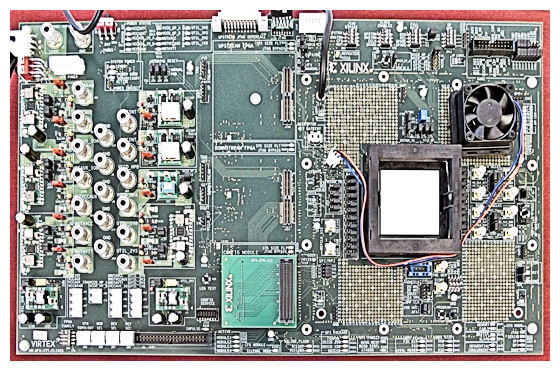
\includegraphics[height=60mm]{Figures/fpga.jpg}

% Title, author and degree
\vspace{0.8cm}
{\FontLb C Compiler for the VERSAT Reconfigurable Processor} \\
\vspace{3.6cm}
{\FontMb Gonçalo da Conceição Reis dos Santos} \\
\vspace{1.9cm}
{\FontLn Thesis to obtain the Master of Science Degree in} \\
\vspace{0.3cm}
{\FontLb Electrical and Computer Engineering} \\
%\vspace{1.9cm}
\vspace{1.0cm}
{\FontSn %
\begin{tabular}{ll}
Supervisor: & Prof. José João Henriques Teixeira de Sousa
\end{tabular} } \\
\vspace{1.0cm}
{\FontMb Examination Committee} \\
\vspace{0.3cm}
{\FontSn %
\begin{tabular}{ll}
Chairperson: & Prof. Francisco André Corrêa Alegria\\
Supervisor: & Prof. José João Henriques Teixeira de Sousa \\
Member of the Committee: & Prof. Paulo Ferreira Godinho Flores \\
\end{tabular} } \\
\vspace{1.5cm}
{\FontMb November 2019} \\
%
\end{center}

\cleardoublepage
 % file "Thesis_FrontCover.tex"

% ----------------------------------------------------------------------
% Dedication page (optional)
% ----------------------------------------------------------------------
%%%%%%%%%%%%%%%%%%%%%%%%%%%%%%%%%%%%%%%%%%%%%%%%%%%%%%%%%%%%%%%%%%%%%%%%
%                                                                      %
%     File: Thesis_Dedication.tex                                      %
%     Tex Master: Thesis.tex                                           %
%                                                                      %
%     Author: Andre C. Marta                                           %
%     Last modified :  2 Jul 2015                                      %
%                                                                      %
%%%%%%%%%%%%%%%%%%%%%%%%%%%%%%%%%%%%%%%%%%%%%%%%%%%%%%%%%%%%%%%%%%%%%%%%

\null\vskip5cm%
\begin{flushright}
     Dedicated to someone special...
\end{flushright}
\vfill\newpage

 % file "Thesis_Dedication.tex"

% ----------------------------------------------------------------------
%  Acknowledgments (optional)
% ----------------------------------------------------------------------
%%%%%%%%%%%%%%%%%%%%%%%%%%%%%%%%%%%%%%%%%%%%%%%%%%%%%%%%%%%%%%%%%%%%%%%%
%                                                                      %
%     File: Thesis_Acknowledgments.tex                                 %
%     Tex Master: Thesis.tex                                           %
%                                                                      %
%     Author: Andre C. Marta                                           %
%     Last modified :  2 Jul 2015                                      %
%                                                                      %
%%%%%%%%%%%%%%%%%%%%%%%%%%%%%%%%%%%%%%%%%%%%%%%%%%%%%%%%%%%%%%%%%%%%%%%%

\section*{\acknowledgments}

% Add entry in the table of contents as section
\addcontentsline{toc}{section}{\acknowledgments}

I want to thank my supervisor, Professor José Teixeira de Sousa, for the 
opportunity to develop this work and for his guidance and support during that process. 
His help was fundamental to overcome the multiple obstacles that I faced during this work.

I also want to acknowledge Professor Horácio Neto for providing a simple Convolutional 
Neural Network application, used as a basis for the application developed for the 
RV32-Versat architecture.

A special acknowledgement goes to my friends, for their continuous support, and Válter,  
that is developing a multi-layer architecture for RV32-Versat. When everything seemed to 
be doomed he always had a miraculous solution.

Finally, I want to express my sincere gratitude to my family for giving me all the 
support and encouragement that I needed throughout my years of study and through the 
process of researching and writing this thesis. They are also part of this work.\\

\textbf{Thank you.}

 % file "Thesis_Acknowledgements.tex"

% ----------------------------------------------------------------------
%  Abstract (both in English and Portuguese)
% ----------------------------------------------------------------------
%%%%%%%%%%%%%%%%%%%%%%%%%%%%%%%%%%%%%%%%%%%%%%%%%%%%%%%%%%%%%%%%%%%%%%%%
%                                                                      %
%     File: Thesis_Resumo.tex                                          %
%     Tex Master: Thesis.tex                                           %
%                                                                      %
%     Author: Carlos A. Rodrigues                                           %
%     Last modified : 21 Jan 2011                                      %
%                                                                      %
%%%%%%%%%%%%%%%%%%%%%%%%%%%%%%%%%%%%%%%%%%%%%%%%%%%%%%%%%%%%%%%%%%%%%%%%

\section*{Resumo}

% Add entry in the table of contents as section
\addcontentsline{toc}{section}{Resumo}

Inserir o resumo em Portugu\^{e}s aqui com o máximo de 250 palavras e acompanhado de 4 a 6 palavras-chave...

\vfill

\textbf{\Large Palavras-chave:} OpenRISC, Sistema em um chip,...

\cleardoublepage

 % file "Thesis_Resumo.tex"
%%%%%%%%%%%%%%%%%%%%%%%%%%%%%%%%%%%%%%%%%%%%%%%%%%%%%%%%%%%%%%%%%%%%%%%%
%                                                                      %
%     File: Thesis_Abstract.tex                                        %
%     Tex Master: Thesis.tex                                           %
%                                                                      %
%     Author: Andre C. Marta                                           %
%     Last modified :  2 Jul 2015                                      %
%                                                                      %
%%%%%%%%%%%%%%%%%%%%%%%%%%%%%%%%%%%%%%%%%%%%%%%%%%%%%%%%%%%%%%%%%%%%%%%%

\section*{Abstract}

% Add entry in the table of contents as section
\addcontentsline{toc}{section}{Abstract}

Versat is a Coarse-Grain Reconfigurable Array architecture (CGRA), which
implements self and partial reconfiguration by using a simple controller
unit. This report studies the current state of the art in HDL and CGRA
simulation, providing a basis to the development of a simulation environment for
Versat. The main objective of this environment is to provide a faster way to
develop and debug software without the use of prototyping hardware. Therefore,
the two types of HDL simulators, event-driven and cycle-accurate, their
advantages and disadvantages are studied, along with a performance comparison
between them. A study of high-level implementations for CGRA simulation is
also presented.

\vfill

\textbf{\Large Keywords:} Versat, coarse-grain reconfigurable arrays, HDL
simulation, CGRA simulation, high-level simulation

 % file "Thesis_Abstract.tex"

% ----------------------------------------------------------------------
%  Table of contents, list of tables, list of figures and nomenclature
% ----------------------------------------------------------------------

% Table of contents
%
\tableofcontents
\cleardoublepage 

% List of tables
%
% Generate list
\listoftables
% Add entry in the table of contents as section
\addcontentsline{toc}{section}{\listtablename}
\cleardoublepage 

% List of figures
%
% Generate list
\listoffigures
% Add entry in the table of contents as section
\addcontentsline{toc}{section}{\listfigurename}
\cleardoublepage 

%% Nomenclature
%%
%% entries of nomenclature list
%%%%%%%%%%%%%%%%%%%%%%%%%%%%%%%%%%%%%%%%%%%%%%%%%%%%%%%%%%%%%%%%%%%%%%%%%
%                                                                      %
%     File: Thesis_Nomenclature.tex                                    %
%     Tex Master: Thesis.tex                                           %
%                                                                      %
%     Author: Gonçalo Santos                                           %
%     Last modified : 20 Oct 2018                                      %
%                                                                      %
%%%%%%%%%%%%%%%%%%%%%%%%%%%%%%%%%%%%%%%%%%%%%%%%%%%%%%%%%%%%%%%%%%%%%%%%
%
% The definitions can be placed anywhere in the document body
% and their order is sorted by <symbol> automatically when
% calling makeindex in the makefile
%
% The \glossary command has the following syntax:
%
% \glossary{entry}
%
% The \nomenclature command has the following syntax:
%
% \nomenclature[<prefix>]{<symbol>}{<description>}
%
% where <prefix> is used for fine tuning the sort order,
% <symbol> is the symbol to be described, and <description> is
% the actual description.

% ----------------------------------------------------------------------
% Roman symbols [r]
\nomenclature[ru]{$\bf u$}{Velocity vector.}
\nomenclature[ru]{$u,v,w$}{Velocity Cartesian components.}
\nomenclature[rp]{$p$}{Pressure.}
\nomenclature[rC]{$C_D$}{Coefficient of drag.}
\nomenclature[rC]{$C_L$}{Coefficient of lift.}
\nomenclature[rC]{$C_M$}{Coefficient of moment.}

% ----------------------------------------------------------------------
% Greek symbols [g]
\nomenclature[g]{$\rho$}{Density.}
\nomenclature[g]{$\alpha$}{Angle of attack.}
\nomenclature[g]{$\beta$}{Angle of side-slip.}
\nomenclature[g]{$\mu$}{Molecular viscosity coefficient.}
\nomenclature[g]{$\kappa$}{Thermal conductivity coefficient.}

% ----------------------------------------------------------------------
% Subscripts [s]
\nomenclature[s]{$x,y,z$}{Cartesian components.}
\nomenclature[s]{$i,j,k$}{Computational indexes.}
\nomenclature[s]{$\infty$}{Free-stream condition.}
\nomenclature[s]{ref}{Reference condition.}
\nomenclature[s]{$n$}{Normal component.}

% ----------------------------------------------------------------------
% Supercripts [t]
\nomenclature[t]{T}{Transpose.}
\nomenclature[t]{*}{Adjoint.}

 % file "Thesis_Nomenclature.tex"
%%
%% Insert glossary/nomenclature section produced by MakeIndex
%\printnomenclature
%% Add entry in the table of contents as section
%\addcontentsline{toc}{section}{\nomname}
%\cleardoublepage

% entries of glossary list
%%%%%%%%%%%%%%%%%%%%%%%%%%%%%%%%%%%%%%%%%%%%%%%%%%%%%%%%%%%%%%%%%%%%%%%%%
%                                                                      %
%     File: Thesis_Glossary.tex                                        %
%     Tex Master: Thesis.tex                                           %
%                                                                      %
%     Author: Carlos A. Rodrigues                                           %
%     Last modified : 30 Oct 2012                                      %
%                                                                      %
%%%%%%%%%%%%%%%%%%%%%%%%%%%%%%%%%%%%%%%%%%%%%%%%%%%%%%%%%%%%%%%%%%%%%%%%
%
% The definitions can be placed anywhere in the document body
% and their order is sorted by <symbol> automatically when
% calling makeindex in the makefile
%
% The \glossary command has the following syntax:
%
% \glossary{entry}
%
% The \nomenclature command has the following syntax:
%
% \nomenclature[<prefix>]{<symbol>}{<description>}
%
% where <prefix> is used for fine tuning the sort order,
% <symbol> is the symbol to be described, and <description> is
% the actual description.

% ----------------------------------------------------------------------

\glossary{name={\textbf{MDO}},description={Multi-Disciplinar Optimization is an engineering technique that uses optimization methods to solve design problems incorporating two or more disciplines.}}

\glossary{name={\textbf{CFD}},description={Computational Fluid Dynamics is a branch of fluid mechanics that uses numerical methods and algorithms to solve problems that involve fluid flows.}}

\glossary{name={\textbf{CSM}},description={Computational Structural Mechanics is a branch of structure mechanics that uses numerical methods and algorithms to perform the analysis of structures and its components.}}

 % file "Thesis_Glossary.tex"

% Insert glossary section produced by MakeIndex
%\printglossary
% Add entry in the table of contents as section
%\addcontentsline{toc}{section}{\glossaryname}
%\cleardoublepage

%acronimos mudar todos os acronimos para o formato como esta o ACK

\vspace*{1.95cm} \hspace*{-0.5cm} %,88
\textbf{{\huge \sffamily Lista de Acrônimos}\\}
\vspace*{0.5cm}
\begin{acronym}
\addcontentsline{toc}{chapter}{Lista de Acrônimos}
\thispagestyle{plain}
\setcounter{page}{13}
\newacronym{soc}{SoC}{\textit{System on Chip}}
\newacronym{uart}{UART}{\textit{Universal Asynchronous Receiver/Transmitter}}
\newacronym{gpio}{GPIO}{\textit{General Purpose Input/Output}}
\newacronym{risc}{RISC}{\textit{Reduced Instruction Set Computing}}
\newacronym{or1200}{OR1200}{\textit{OpenRISC12000}}
\newacronym{fpga}{FPGA}{\textit{Field Programmable Gate Array}}
\newacronym{jtag}{JTAG}{\textit{Joint Test Action Group}}
\newacronym{orpsoc}{ORPSoC}{\textit{OpenRISC Reference Platform System-on-Chip}}
\newacronym{ads}{ADS}{\textit{Advenced Debug System}}
\newacronym{usb}{USB}{\textit{Universal Serial Bus}}
\newacronym{openocd}{OpenOCD}{\textit{Open On-Chip Degugger}}
\newacronym{rsp}{RSP}{\textit{Remote Serial Protocol}}
\newacronym{bios}{BIOS}{\textit{Basic Input Output System}}
\newacronym{fifo}{FIFO}{\textit{Frist In First Out}}
\newacronym{i2c}{I2C}{\textit{Inter-Integrated Circuit}}
\newacronym{scl}{SCL}{\textit{Serial Clock}}
\newacronym{sda}{SDA}{\textit{Serial Data}}
\newacronym{spi}{SPI}{\textit{Serial Peripheral Interface}}
\newacronym{sclk}{SCLK}{\textit{Serial Clock}}
\newacronym{mosi}{MOSI}{\textit{Master Out Slave In}}
\newacronym{miso}{MISO}{\textit{Master In Slave Out}}
\newacronym{ss}{SS}{\textit{Slave Select}}
\newacronym{sd}{SD}{\textit{Security Digital}}
\acro{ACK}{Acknowledge}
\end{acronym}
\cleardoublepage
% Set arabic numbering (1,2,...) after preface
%
\setcounter{page}{1}
\pagenumbering{arabic}

% ----------------------------------------------------------------------
%  Chapters
% ----------------------------------------------------------------------

%%%%%%%%%%%%%%%%%%%%%%%%%%%%%%%%%%%%%%%%%%%%%%%%%%%%%%%%%%%%%%%%%%%%%%%%
%                                                                      %
%     File: Thesis_Introduction.tex                                    %
%     Tex Master: Thesis.tex                                           %
%                                                                      %
%     Author: Andre C. Marta                                           %
%     Last modified :  2 Jul 2015                                      %
%                                                                      %
%%%%%%%%%%%%%%%%%%%%%%%%%%%%%%%%%%%%%%%%%%%%%%%%%%%%%%%%%%%%%%%%%%%%%%%%

\chapter{Introduction}
\label{chapter:introduction}




In this report, the problem of accelerating the execution of Deep Neural
Networks (DNNs) using Coarse GRained Reconfigurable Arrays (CGRAs) is studied,
with special emphasis on compiling a DNN description into code that runs on
CPU/CGRA system. The Deep Versat Architecture~\cite{valter:deepversat} CGRA will be used as an
implementation tool in this work.


%%%%%%%%%%%%%%%%%%%%%%%%%%%%%%%%%%%%%%%%%%%%%%%%%%%%%%%%%%%%%%%%%%%%%%%%
\section{Problem}
\label{section:problem}

Neural Networks have been an object of study since the 1940's, but until the
beginning of this decade their applications were limited and did not play a
major role in computer vision conferences. With its meteoric rise in research,
several solutions to accelerate this algorithm have appeared, from Field Programmable Gate Arrays (FPGA) to
Application Specific Integrated Circuits (ASIC) implementations.

Convolutional Neural Networks (CNNs) are a particular kind of DNN where the output
values of the neurons in one layer are convolved with a kernel to produce the
input values of the neurons of the next layer. This algorithm is compute bound,
that is, its performance depends on how fast it can do certain calculations, and
depend less on the memory access time. Namely the convolutional layers take
approximately 90$\%$ of the computation time.

The acceleration of these workloads is a matter of importance for today's
applications such as image processing for object recognition or simply to
enhance certain images. Other uses like instant translation and virtual
assistants are applications of neural networks and their acceleration is of
vital importance to bring them into Internet of Things.

A suitable circuit to accelerate DNNs in hardware is the CGRA. A CGRA is a
collection of Functional Units and memories with programmable interconnections
in order to form computational datapaths. A CGRA can be implemented in both
FPGAs and ASICs. CGRAs can be reconfigured much faster than FPGAs, as they have
much less configuration bits. If reconfiguration is done at runtime, CGRAs add
temporal scalability to the spacial scalability that characterize
FPGAs. Moreover, partial reconfiguration is much easier to do in CGRAs compared
to FPGAs which further speeds up reconfiguration time. Another advantage of
CGRAs is the fact that they can be programmed entirely in software, contrasting
with the large development time of customized Intellectual Property (IP) blocks.
The Coarse Grain Reconfigurable Arrays (CGRA) is a midway acceleration solution
between FPGAs, which are flexible but large, power hungry and difficult to
reprogram, and ASICs, which are fast but generally not programmable.

However, mapping a specific DNN to a CGRA requires knowledge of its
architecture, latencies and register configurations, which may become a lengthy
process, especially if the user wants to explore the design space for several
DNN configurations. An automatic compiler that can map a standard DNN
description into CPU/CGRA code would dramatically decrease time to market of its
users. Currently there are equivalent tools for CPUs and GPUs and
even for FPGAS.


%%%%%%%%%%%%%%%%%%%%%%%%%%%%%%%%%%%%%%%%%%%%%%%%%%%%%%%%%%%%%%%%%%%%%%%%
\section{Solution}
\label{section:solution}

The proposed solution is a compiler that takes a configuration file from a
neural network framework like Caffe or Darknet. This new tool inputs the
parameters of Deep Versat, such as the number of layers and functional units,
and produces the C code needed for the Versat runs. This code is run on the
RISC-V picorv32~\cite{picorv} CPU controller that has Deep Versat as a peripheral.

%%%%%%%%%%%%%%%%%%%%%%%%%%%%%%%%%%%%%%%%%%%%%%%%%%%%%%%%%%%%%%%%%%%%%%%%
%\section{Thesis Outline}
%\label{section:outline}

%Briefly explain the contents of the different chapters...

%%%%%%%%%%%%%%%%%%%%%%%%%%%%%%%%%%%%%%%%%%%%%%%%%
%\section{Author's Work}
%\label{section:authorwork}

%TO ADD----

%%%%%%%%%%%%%%%%%%%%%%%%%%%%%%%%%%%%%%%%%%%%%%%%%%
\section{Report Outline}
\label{reportoutline}

This report is composed of 4 more chapters. In the second chapter, the
state-of-the-art of neural networks and the difficulties accelerating them is
described. In the third chapter, the Deep Versat architecture and how to program
it is explained. In the fourth chapter, CNN compiler techniques are
explored. Finally, the last chapter contains the proposed solution and the plan
for its execution.


 % file "Thesis_Introduction.tex"

\chapter{Estado-da-arte}
\label{chapter:estadodaarte}

Existem duas maneiras de desenvolver o \acrshort{soc} desenvolvendo um sistema por completo incluindo processador, bus de comunicação, protocolos de comunicação necessários, que torna complicado a idealizar e desenvolver no tempo disponível para a sua execução. Ou juntamo-nos a uma das várias comunidades Open Hardware (open source de hardware) já existentes onde já tem algumas das funcionalidades idealizadas ou desenvolvidas, ainda permitindo contribuir para a comunidade escolhida com alguns melhoramentos ou resoluções de problemas existem nos seus projectos.

%http://en.wikipedia.org/wiki/OpenCores
Das maiores comunidades de open source de hardware é a OpenCores, com aproximadamente 800 projectos e 95 mil utilizadores registados em 2010. Os projectos desenvolvidos por esta comunidade por serem no desenvolvimento de hardware usam uma linguagem de descrição de hardware na maioria dos projectos da comunidade são desenvolvidos em Verilog uma das linguagens mais utilizadas na descrição de hardware.

\section{OpenRISC}
\label{section:OpenRisc}

%opencores.org/websvn,filedetails?repname=openrisc&path=%2Fopenrisc%2Ftrunk%2Fdocs%2Fopenrisc-arch-1.1-rev0.pdf
%http://opencores.org/or1k/OR1K:Community_Portal
%http://en.wikipedia.org/wiki/OpenRISC

O principal projecto inicial da comunidade é o projecto OpenRISC, tem como objectivo desenvolver uma serie de processadores com a arquitetura \acrlong{risc}.

 A primeira discrição arquitectura é para o projecto OpenRISC1000, sendo um processador de 32 ou 64 bits com a opção de ponto flutuante e suporte para um processamento vectorial. A equipa OpenCores fez a primeira aplicação de um \acrshort{soc} com um processador deste tipo dando-lhe o nome \acrlong{or1200} este é escrito em verilog sintetizavel e tem um capacidade de processamento semelhante ao processador ARM10. Varias empresas desenvolvem os seus processadores com base neste processador entre as mais conhecidas estão a Samsung e a Nasa. 

%http://opencores.org/or2k/OR2K:Community_Portal
A discrição do segundo projecto de processadores com o nome OpenRISC2000 pretende ser um sucessor do anterior sendo as características principais compatível com o projeto anterior, projeto modular, adaptado para o uso de multicores, destinado para o embebido ou seja para dados de 16 e 32 bits sem suporte para 64 bits e desenvolvido para pequenos e médios processadores de \acrlong{fpga}


\subsection{Arquitectura}
%http://www.rte.se/blog/blogg-modesty-corex/openrisc-1200-soft-processor
%http://en.wikipedia.org/wiki/OpenRISC_1200
%http://opencores.org/or1k/OR1200_OpenRISC_Processor

Na arquitectura desde processador como se pode ver na figura \ref{figures:or1200} o processador tem disponível unidade de debug permitindo um realizar-se debug em tempo real onde é ligado um de \acrlong{jtag}, \textcolor[rgb]{1,0,0}{tick timer} de alta resolução, controlador de interrupções programáveis, gestor de energia e uma cache e uma unidade de gestão de memoria tanto para instruções como para dados. Estas unidades mencionadas têm a hipótese de serem facilmente removidas caso não sejam necessárias permitindo assim que o processador tem uma tamanho menor e um consumo menor de energia. Para alem desta unidade opcionais existem duas outras unidas designadas Wishbone que pertencer a arquitectura base do processador, uma pertence a interface de instruções e a outra a interface de dados. Estas duas unidades fazem a conversão da interface interna RISC para a interface Wishbone que é recebida pelos periféricos.


\begin{figure}[!htb]
  \centering
  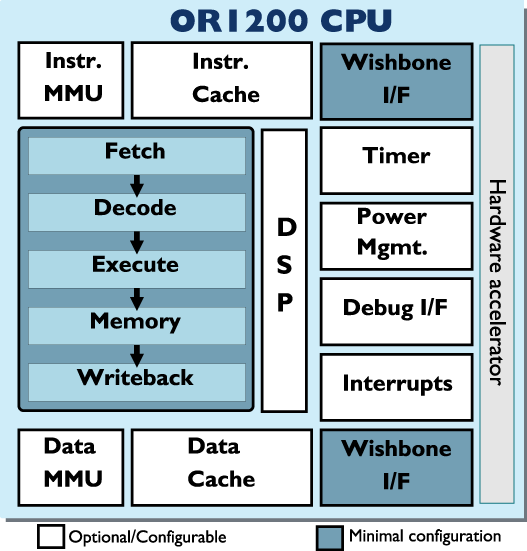
\includegraphics[width=0.5\textwidth]{Figures/Or1200_blocks.png} %1
  \caption[Diagrama de blocos do processador OpenRISC1200]{Diagrama de blocos do processador OpenRISC1200}
  \label{figures:or1200}
  %http://opencores.org/or1k/OR1200_OpenRISC_Processor
\end{figure}  

\subsection{Arquitectura Wishbone}
\label{section:wishbone}
% cdn.opencores.org/downloads/wbspec_b4.pdf
% http://opencores.org/opencores,wishbone
%http://www.google.com/url?sa=t&rct=j&q=&esrc=s&source=web&cd=10&cad=rja&uact=8&ved=0CG4QFjAJ&url=http%3A%2F%2Fairccse.org%2Fjournal%2Fvlsi%2Fpapers%2F3212vlsics10.pdf&ei=uMS7U5OdB6PA7AappYDICQ&usg=AFQjCNF6tg65Fvsk68LRwCc0towm93uTRw&bvm=bv.70138588,d.ZGU  ver melhor
% http://www.pldworld.com/_hdl/2/_ip/-silicore.net/wishbone.htm

A interface de barramento wishbone é hardware opensource, permitindo comunicação entre varias partes de um circuito integrado com o objetivos de ligar diferentes cores dentro de um chip. A interface é bastante utilizada em CPU e periféricos opensource, onde se destacam muitos dos projectos da comunidade OpenCores. A comunidade recomenda que todos os cores tenham disponível uma interface wishbone. O barramento wishbone foi desenvolvido pela silicore corporation em 1999 disponibilizando para domínio publico  uma biblioteca em VDHL, a partir de 2002 a comunidade OpenCores tornou-se também sponsors do wishbone tendo uma pagina dedicada onde estão disponível novas revisões. 

Existem várias interfaces possíveis com a arquitectuta wisbone os 4 tipos mais habituais podem ser visto na figura \ref{Figure:I_wishbone}. A interligação ponto a ponto, na figura \ref{Figure:I_wishbone_a}, permite apenas uma ligação de um periférico, este tipo de ligação não normalmente utilizada em \acrshort{soc} por estes normalmente serem constituídos por vários periféricos. A interface de barramento partilhado, na figura \ref{Figure:I_wishbone_b}, permite a utilização de vários mestres e vários escravos, visto que o barramento é partilhado o quanto um mestre utiliza o barramento o outro escravo tem de esperar que fique disponível o controlo é feito por um arbitro que decidi que arbrito controlo o barramento naquele momento. No caso do comutador de barra , na figura \ref{Figure:I_wishbone_c},é utilizado para uma tipologia multi-core. Este permite uma comunicação entre dois mestres e os escravos ao mesmo tempo desde que estejam a aceder a escravos diferentes, é semelhante ao barramento partilhado com uma elevada taxa de transferência de dados. Por ultimo a interligação de fluxos de dados, na figura \ref{Figure:I_wishbone_d}, a informação flui de periférico para periférico, todos os periféricos têm de ter a interface de escravo e de mestre.

\begin{figure}[!htb]
  \begin{subfigmatrix}{4}
    \subfigure[Interligação ponto a ponto]{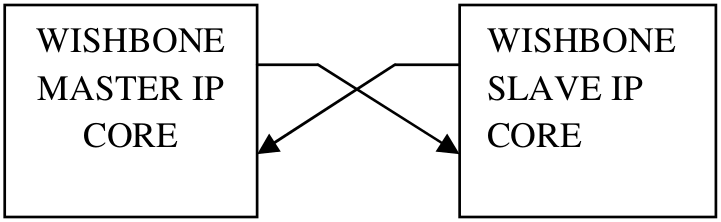
\includegraphics[width=0.49\linewidth]{Figures/wishbone_PP.png}\label{Figure:I_wishbone_a}}
    \subfigure[Interligação de barramento partilhado]{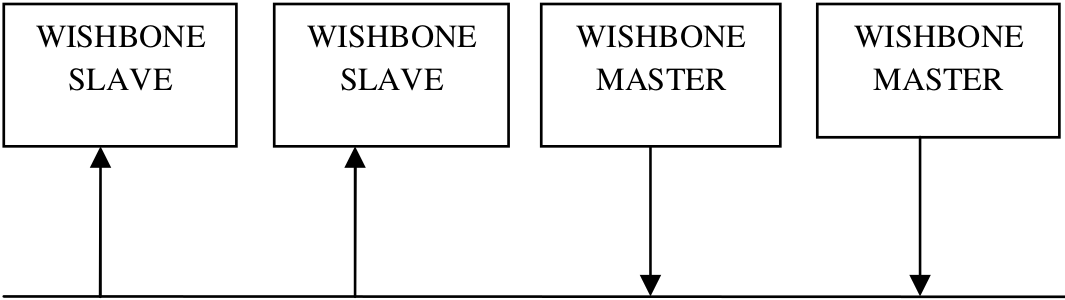
\includegraphics[width=0.49\linewidth]{Figures/wishbone_bus.png}\label{Figure:I_wishbone_b}}
    \subfigure[Interligação comutador de barra(crossbar swith)]{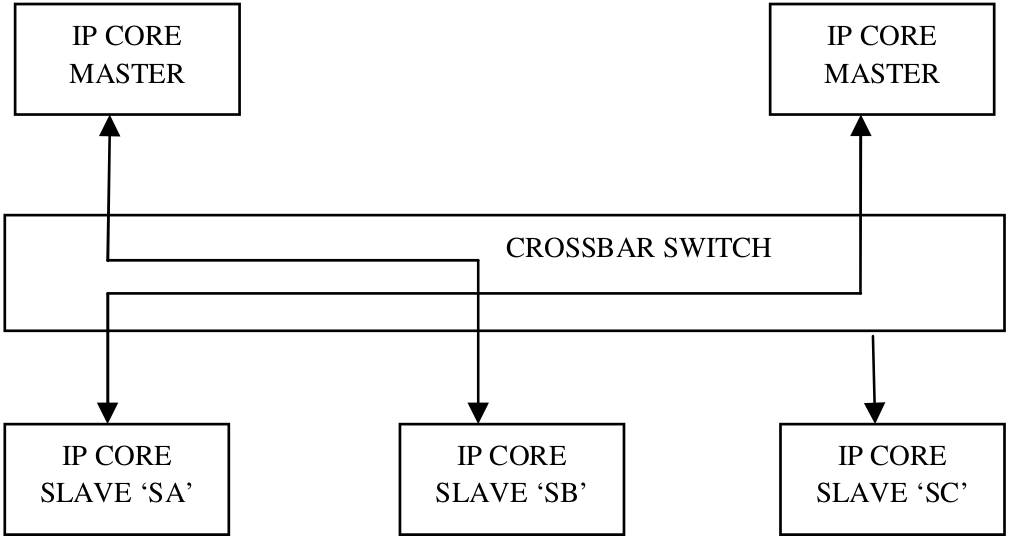
\includegraphics[width=0.49\linewidth]{Figures/wishbone_switch.png}\label{Figure:I_wishbone_c}}
    \subfigure[Interligação de fluxo de dados]{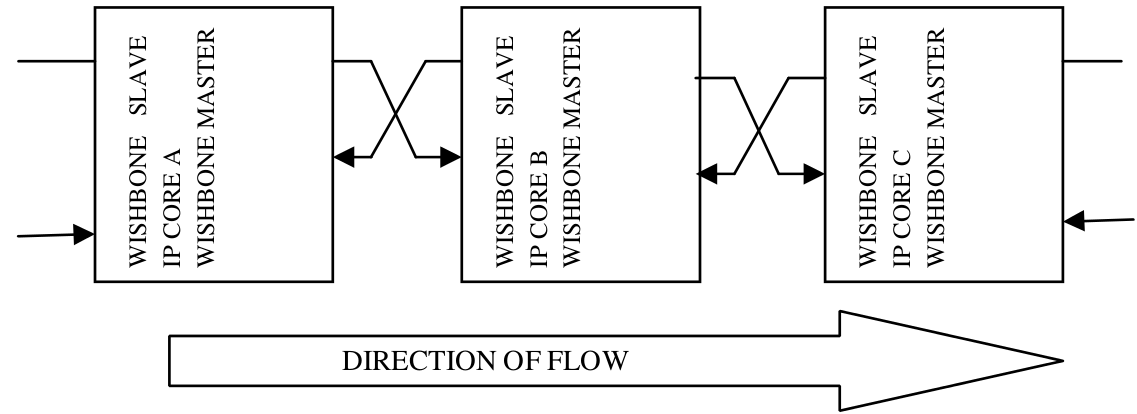
\includegraphics[width=0.49\linewidth]{Figures/wishbone_flow.png}\label{Figure:I_wishbone_d}}
  \end{subfigmatrix}
  %http://www.google.com/url?sa=t&rct=j&q=&esrc=s&source=web&cd=10&cad=rja&uact=8&ved=0CG4QFjAJ&url=http%3A%2F%2Fairccse.org%2Fjournal%2Fvlsi%2Fpapers%2F3212vlsics10.pdf&ei=uMS7U5OdB6PA7AappYDICQ&usg=AFQjCNF6tg65Fvsk68LRwCc0towm93uTRw&bvm=bv.70138588,d.ZGU 
  \caption{Interfaces Wishbone}
  \label{Figure:I_wishbone}
\end{figure}

A interligação utilizada no desenvolvimento de \acrshort{soc} com apenas uma unidade de processamento é o barramento partilhado, porque tem vários periféricos disponíveis e por ser de simples implementação. Onde é feita toda a gestão da interface wishbone é dado o nome Intercon, este é constituído por vários elementos como multiplexer e árbitros wishbone. Como se pode ver na figura \ref{grafos:wishbone} ambos os modelos de wishbone do processador mencionados na figura \ref{figures:or1200} estão ligados cada um deles a um multiplexer um de dados e outro de instruções, estes enviam os dados para o periférico correspondente conforme o escalonamento atribuído a cada periférico. Existe uma ligação de ambos os multiplexeres ao árbitro este faz o controlo dos acessos à memoria principal, pois é possível aceder a memoria principal por necessitar de novas instruções como de necessitar de dados lá existentes. Os sinais da interface wishbone encontram-se descritos na tabela\ref{table:wishbone}, na tabela a direcção dos sinais mencionados visto do periférico escravo.

Para adicionar um novo periférico ao \acrshort{soc} que tem disponível uma interface wishbone, a interface do escravo é ligada ao multiplexer de wishbone de dados à semelhança dos outros periféricos ligados na figura \ref{grafos:wishbone}, tem de ser atribuído ao periférico um conjunto de endereços disponíveis.

\begin{figure}[!htb]
  \centering
  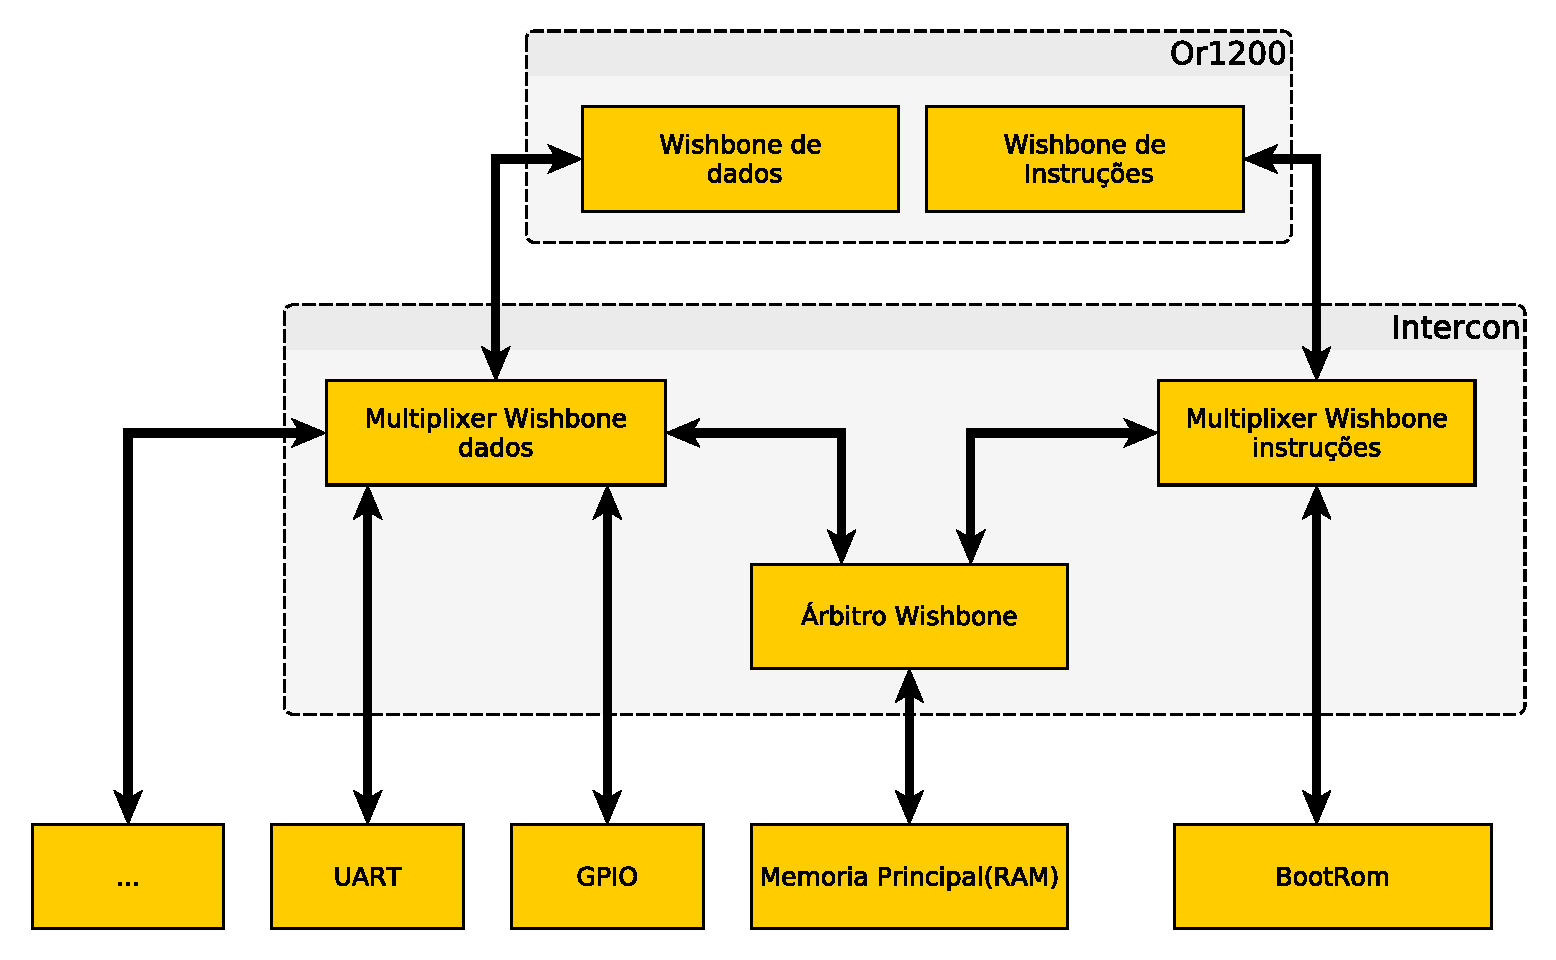
\includegraphics[width=0.5\textwidth]{grafos/wishbone.pdf} %1 será que não devo por sem ROM (como estava originalmente)
  \caption[Diagrama de blocos da arquitectura wishbone.]{Diagrama de blocos da arquitectura wishbone.\textcolor[rgb]{1,0,0}{por esta figura mais completa ou uma como estava originalmente, sem bootrom}}
  \label{grafos:wishbone}
\end{figure} 

A interface wishbone é constituida por 12 sinais distintos que se encontram descritos na tabela \ref{table:wishbone}, a maior parte dos sinais com a excepção de wbm\_adr\_i, wbm\_dat\_i, wbm\_dat\_o e wbm\_sel\_i são de apenas um bit e não variam o tamanho de bits conforme a quantidade de bits do \acrshort{soc}. na tabela mostra os sinais visto do lado do periférico.

\begin{table}[h!]
  \begin{center}
    \begin{tabular}{|c|c|c|c|}
      \hline
      Nome & Direcção & Tamanho(bits) & Descrição \\
      \hline \hline
      wbm\_cki\_i & Input & 1 & Clock do sistema para a interface Wishbone. \\
      \hline
      wbm\_rst\_i & Input & 1 & Sinal de Reset (activo com valor lógico '1'). \\ 
      \hline
      wbm\_cyc\_i & Input & 1 & Validação da informação no Bus.\\ % ver
      \hline
      wbm\_adr\_i & Input & 32 & Endereço para escrita ou leitura no periférico.\\
      \hline
      wbm\_dat\_i & Input & 32 & Dados enviados para o periférico.\\
      \hline
      wbm\_dat\_o & Output & 32 & Dados enviados pelo periférico.\\
      \hline
      wbm\_sel\_i & Input & 4 & Seleciona Byte para escrever ou ler.\\ % ver
      \hline
      wbm\_ack\_o & Output & 1 & Sinal de acknowledgment. \\
      \hline
      wbm\_err\_o & Output & 1 & Indica um ciclo anormal ocorreu um encerramento.\\
      \hline
      wbm\_we\_i & Input & 1 & sinal de leitura ou escrita, se tiver logico '1' escreve.\\
      \hline
      wbm\_stb\_i & Input & 1 & Valida os dados transmitidos.\\
      \hline
      wbm\_rty\_0 & Output & 1 & \\
      \hline
    \end{tabular}
  \end{center}
  \caption[Tabela dos sinais da interface Wishbone.]{Tabela dos sinais da interface Wishbone.}
  \label{table:wishbone}
\end{table} 

A interface Wishbone mestre é controlada pela elemento Data ou Instr. Cache, dependendo se se trata da interface de dados ou de instruções respectivamente, que pode ser visto na figura \ref{figures:or1200}. Ai a leitura e as escritas para podem ser simples, leitura de apenas uma posição de memoria, ou brust, uma sequencia de posições de memória, em brust são feitas 4 acessos a memorias sequenciais, isto é definido está definido no código e corresponde ao tamanho do MMU correspondente. Na figura \ref{ondas:wishbone} podem-se ver vários diagrama temporais de leituras e escritas do elemento Cache.

Nas figuras \ref{ondas:wishbone_a} e \ref{ondas:wishbone_b} corresponde a diagramas temporais lidos no elemento Data Cache, o sinal dcfsm\_burst aciona uma leitura ou escrita em burst. Na primeira figura temos uma leitura simples, como se pode ver o sinal de burst está com o valor lógico de 'zero' e o sinal biu\_sel\_i tambem se encontra com o valor logico de  'zero' indicando que é uma leitura. Também se pode ver que o sinal biu\_sel\_i é o primeiro a ser definido e tem o valor 4 em hexadecimal, indicando que é para ser lido apenas 2 Bytes e são para ser coculados nos 2 Bytes mais significativos do sinal biu\_dat\_o.

Na figura \ref{ondas:wishbone_b} temos uma escrita simples, neste caso ainda temos o sinal dcfsm\_burst com o valor logico de 'zero', mas biu\_we\_i já tem o valor lógico de 'um' acionado ao mesmo tempo que os sinais biu\_cyc\_i e biu\_stb\_i. Já neste caso o sinal biu\_sel\_i com o valor F em hexadecimal indica que todos os bytes de biu\_dat\_i são validos.

Por ultimo na figura \ref{ondas:wishbone_c} é um diagrama temporal do elemento Instr. Cache, onde é representado uma leitura em burst. Neste caso podemos ver que o sinal icfsm\_burst tem o valor logico 'um', também se pode ver no sinal biu\_adr\_i que o endereço se mantem até receber o primeiro ACK a partir dai é incrementado de 4 em 4 posições de memoria em cada flanco ascendente visto que o periférico disponibiliza a palavra e que ao fim de receber 4 palavras o sinal de burst fica com o valor logico de 'zero'.

\begin{figure}[!htb]
  \begin{subfigmatrix}{3}
    \subfigure[Diagrama temporal do ciclo de leitura simples]{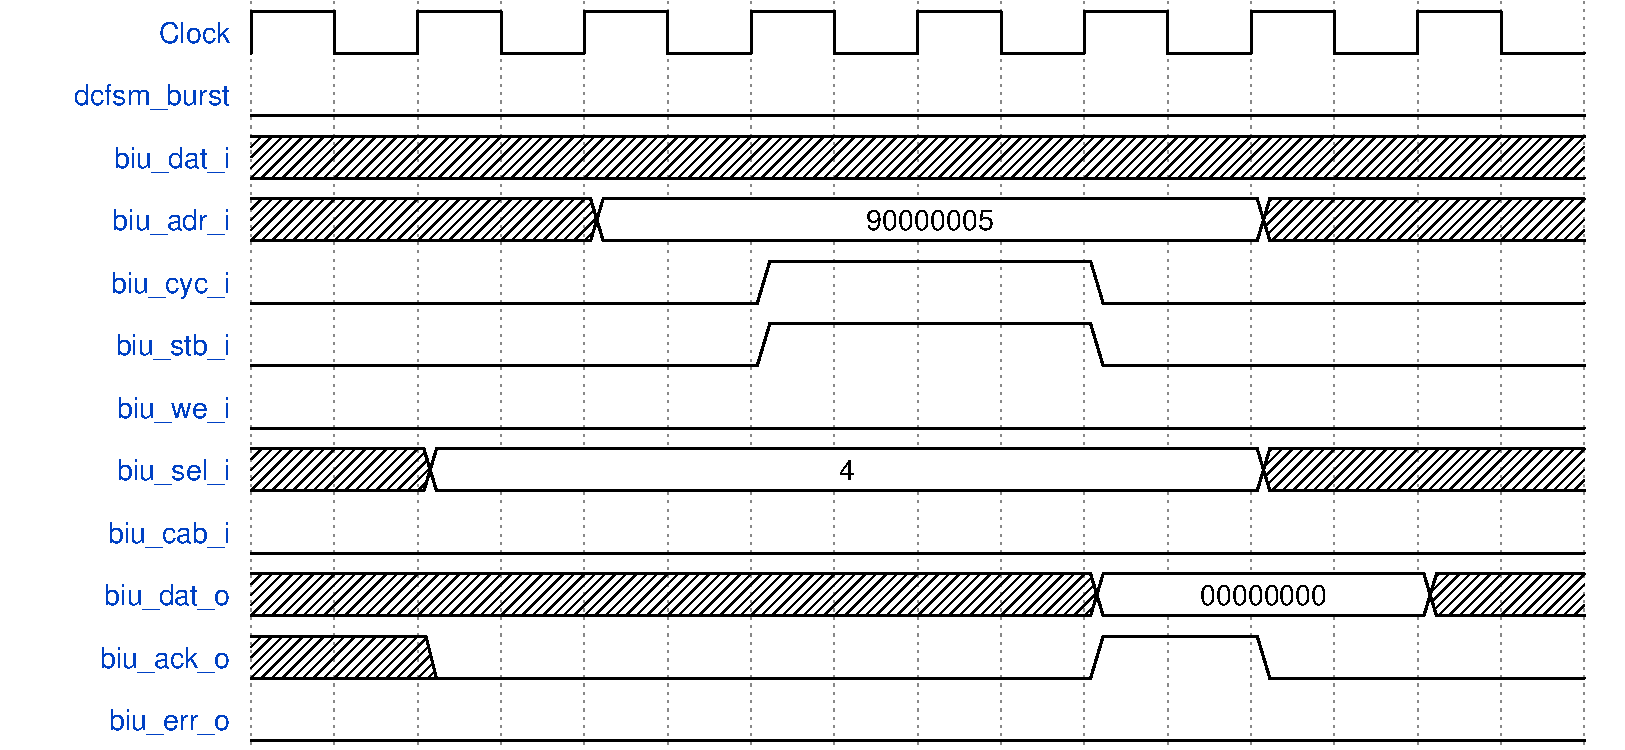
\includegraphics[width=0.49\linewidth]{ondas/wishbone_R_single.pdf}\label{ondas:wishbone_a}}
    \subfigure[Diagrama temporal do ciclo de escrita simples]{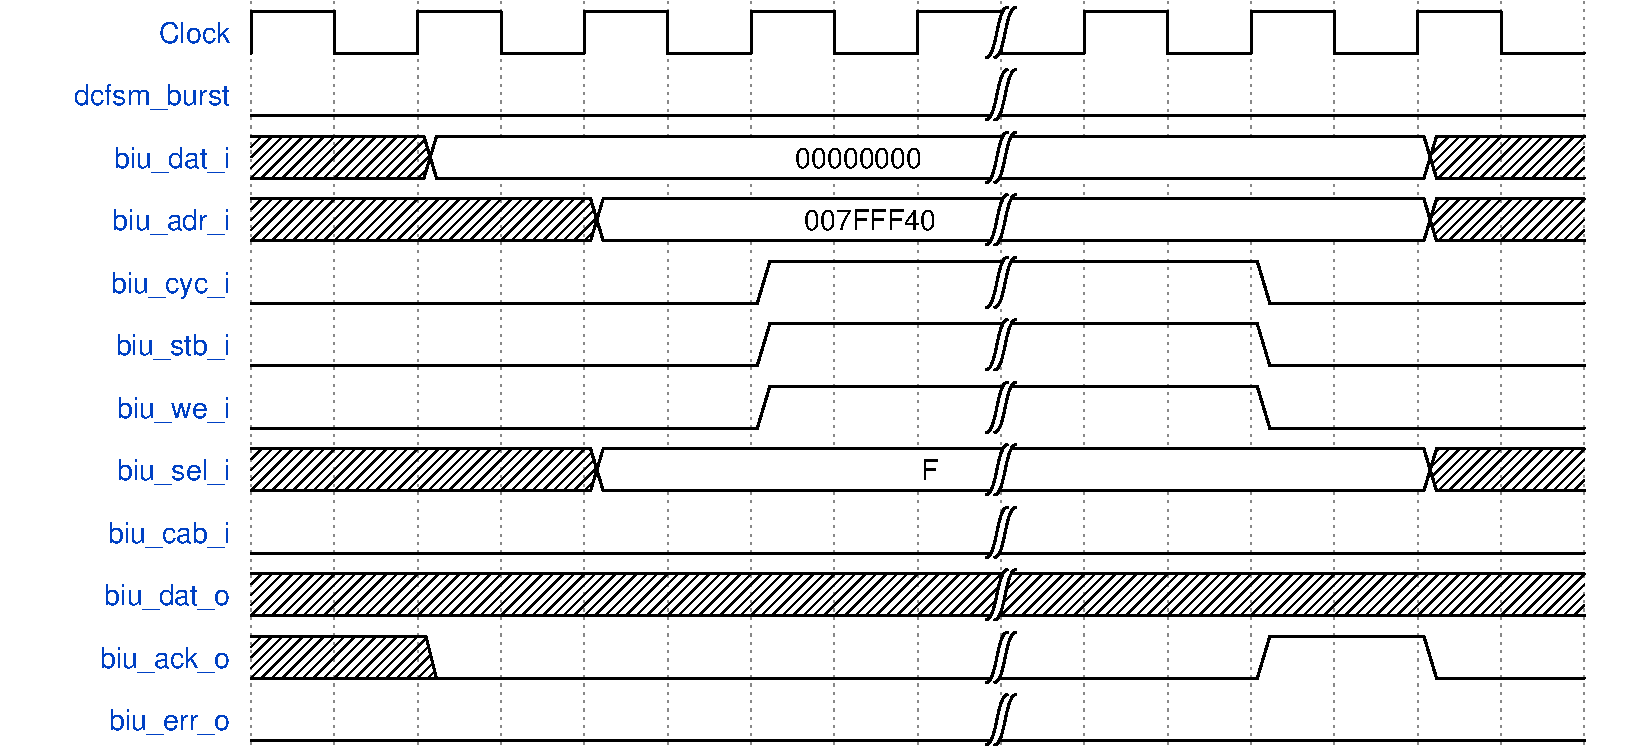
\includegraphics[width=0.49\linewidth]{ondas/wishbone_W_single.pdf}\label{ondas:wishbone_b}}
    \subfigure[Diagrama temporal do ciclo de leitura burst]{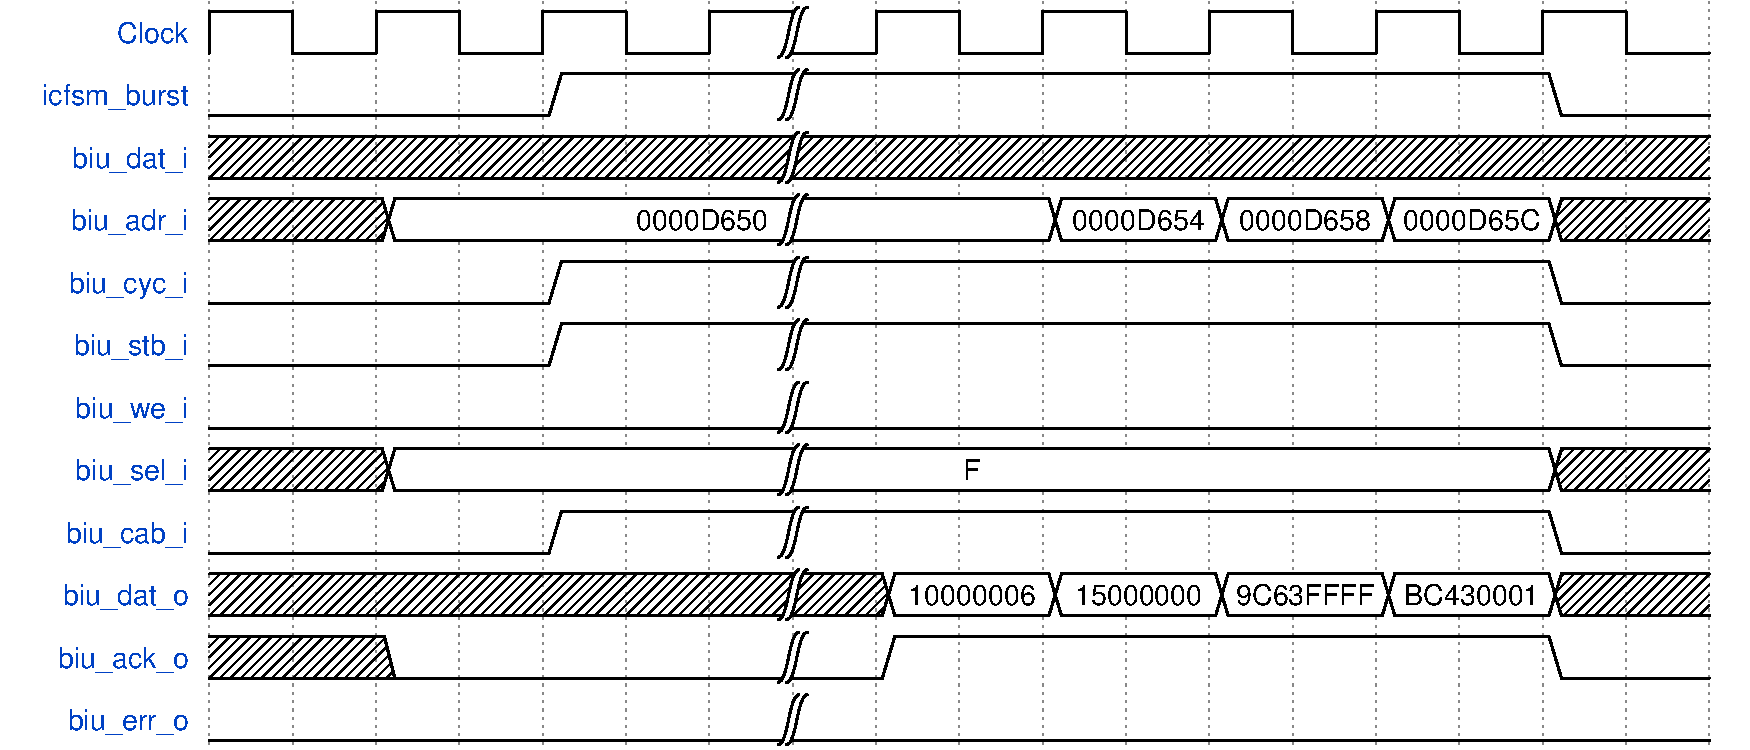
\includegraphics[width=0.49\linewidth]{ondas/wishbone_R_burst.pdf}\label{ondas:wishbone_c}}
  \end{subfigmatrix} 
  \caption{Diagrama temporais Wishbone}
  \label{ondas:wishbone}
\end{figure}

\subsection{Toolchain}

% http://elinux.org/Toolchains
% http://en.wikipedia.org/wiki/Toolchain
% http://en.wikipedia.org/wiki/GNU_toolchain
Uma Toolchain é um conjunto de ferramentas de programação que permitem criar programas, vulgarmente uma toolchain simples disponível um compilador, um linker para fazer a linkagem do código compilado para um programa executável, bibliotecas que fornecem interface com o sistemas operativo e um debugguer. Uma das toolchain mais utilizadas para desenvolver programas em C é a toolchian da GNU sendo vital para o desenvolvimento de linux, alguns sistemas BSD e software para sistemas embebidos. A toolchain da GNU disponibliza mais algumas ferramentas do que uma simples toochain, como uma ferramenta para compilação automática vulgarmente conhecida por Make.

% http://opencores.org/or1k/OpenRISC_GNU_tool_chain#Linux_.28uClibc.29_toolchain_.28or1k-linux-uclibc.29
% http://www.uclibc.org/about.html
% http://opencores.org/or1k/Newlib
Por ser uma toolchain bastante utilizada em desenvolvimento de software a comunidade utiliza a toolchain da gnu para desenvolver software, mas o processador ainda não é suportado pela toolchain. A comunidade adicionou o seu processador em duas bibliotecas na newlib e na uClibc, a newlib é uma biblioteca já testada e utilizada desde a versão 1.18.0 com suporte de placas, sendo uma pequena e simples biblioteca de C do que uClibc e é a melhor para o desenvolvimento de aplicações em bare-metal ou seja sem sistema operativo. uClibc é um biblioteca de C para sistemas embebidos onde foi removido algumas partes do padrão de C, mas ainda dispoen de todas a funcionalidades necessarias para um sistema operativo, é ideal para sistema embebidos suportando ARM, amd64,i386.

% http://opencores.org/or1k/Newlib --> fala das boards
% http://opencores.org/or1k/OpenRISC_GNU_tool_chain
A biblioteca newlib é utilizada no desenvolvimento de aplicação em bare-metal por isso é necessário indicar ao compilador para fazer a linkagem. Para esse efeito existe a flag "-mboard" onde se indica qual é a placa onde o o programa irá correr. Existem já algumas placas predefinidas como or1ksim, simulador or1ksim sem \acrlong{uart}, or1ksim-uart, simulador or1ksim com \acrshort{uart}, de0\_nano, placa \acrshort{fpga} de0 nano da Terasic. Quando indicamos com a flag qual é a placa que utilizamos o compilador irá buscar um ficheiro com o mesmo nome já précompilado que contem informações importante da placa que são frequencia de clock, endereço base da memoria principal, tamanho da memoria principal, endereço base da \acrshort{uart}, buad rate da \acrshort{uart} e o numero IRQ da \acrshort{uart}. É possivel criar um ficheiro com as propriedades da placa que pretender para isso tem de criar um ficheiro com o nome da placa com a extensão .S. % ver como se compila o ficheiro.s

\subsection{OrpSoc}
\label{section:orpsoc}
%http://opencores.org/or1k/ORPSoCv3
% http://opencores.org/or1k/ORPSoCv2
% http://opencores.org/or1k/ORPSoC
No desenvolvimento do \acrshort{soc} a comunidade OpenRISC percebeu-se da necessidade de uma plataforma de desenvolvimento fácil e modelar. Por esses motivos desenvolveram o \acrlong{orpsoc} destinando-se a desenvolver um ambiente de verificação e de desenvolvimento de Cores IP ou \acrshort{soc}. Para alem dos principais objectivos teria de ser simples de usar tanto por utilizadores experimentes como por utilizadores novos, permitindo este simular e sintetizar o seu projeto facilmente. A plataforma encontrasse separada do repositório onde se encontra os sistemas e os cores, permitindo assim que a plataforma seja utilizada com \acrshort{soc} totalmente diferentes e por outras \textcolor[rgb]{1,0,0}{identidades}.

O repositório onde se encontram os sistemas e os cores têm uma distribuição como se encontra na figura \ref{grafos:orpsoc}, no caso da OpenRISC o repositório tem o nome de Orpsoc-cores. Dentro do repositório existe mais dois com os nomes de cores e systems, dentro do repositório systems estão todos os \acrshort{soc} desenvolvidos ou em desenvolvimento cada um com o teu repositório especifico, dentro de cada \acrshort{soc} existem vários ficheiros sendo 2 deles bastante importantes que têm de ter o nome do sistema com as extensões .core e .system, por exemplo de0\_nano.core e de0\_nano.system no caso que seja o sistema de0\_nano. O ficheiro .system tem descrição sobre o sistema e a localização dos ficheiros necessários para sintetizar o sistemas para uma determinada \acrshort{fpga}. No caso do ficheiro .core contem toda as dependências do sistema em relação aos cores, tendo também secção das várias ferramentas de simulação onde cada uma descrimina informações necessárias para a sua compilação, como ficheiros de testbench, flags de compilação e o ficheiro principal.

Quanto ao repositórios cores contem vários cores onde cada um tem o seu repositório onde é obrigatório ter o ficheiro com a extensão .core que contem a uma descrição do core, dependência de outros cores e os ficheiros de descrição do core. É possível que os ficheiros de discrição não estejam no repositório, nesse caso o ficheiro também contem um secção que indica a sua localização no servidor de Subversion da comunidade e qual a revisão, neste caso a plataforma \acrlong{orpsoc} também tem a responsabilidade de fazer uma copia deste core. 


\begin{figure}[!htb]
  \centering
  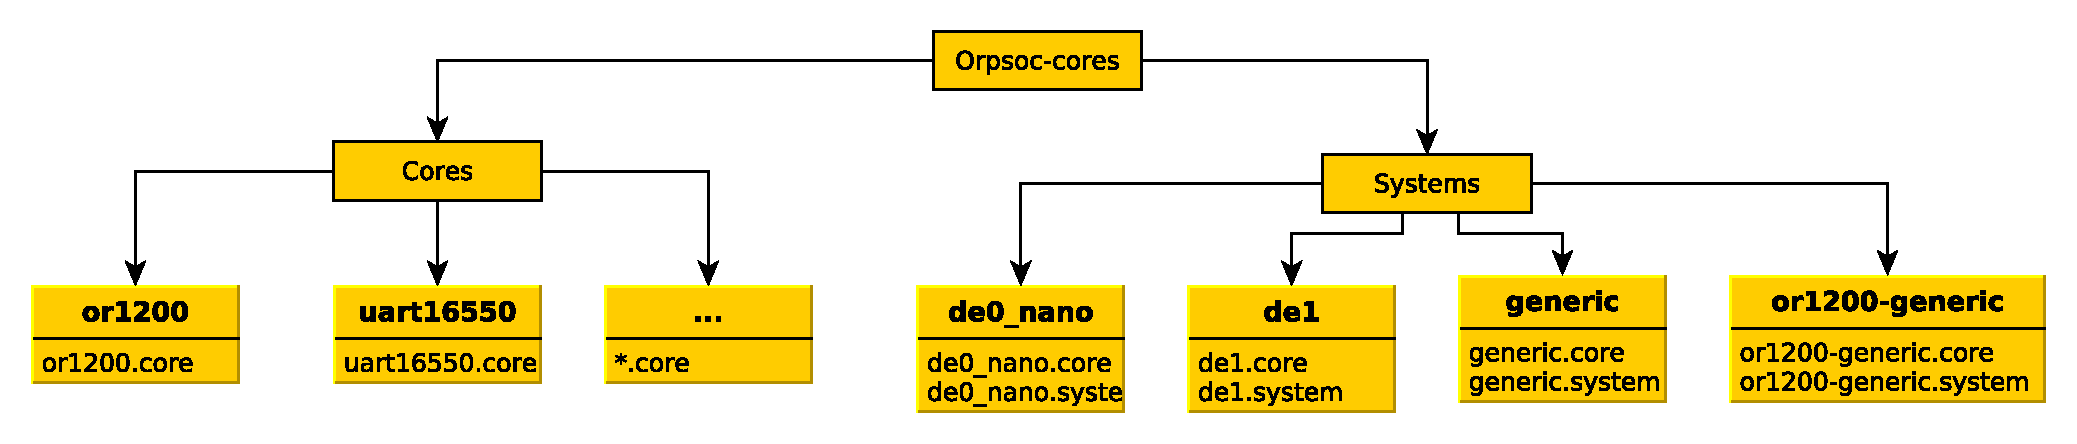
\includegraphics[width=1.0\textwidth]{grafos/orpsoc-cores.pdf} %0.5
  \caption[Organização do sistemas e cores da OpenRisc]{Organização do sistemas e cores da OpenRisc.}
  \label{grafos:orpsoc}
\end{figure} 

Cada sistema que se encontra no repositório systems onde pode ser visto na figura \ref{grafos:orpsoc} é constituídos por vários cores que se encontram no repositório cores. Cada core pode depender ou não de um ou mais cores. Um core descreve como é um elemento, como processador ou periférico. Um sistemas descreve como esses cores estão interligados entre si. Tornando assim a criação de novos sistemas que podem usar o mesmo cores que outro sistema, não sendo necessário ter duas copias do mesmo core e sendo mais fácil manter os cores actualizados.

Na figura \ref{grafos:fusesoc} representa o sistema de ficheiros existente no ORPSoC. Encontra-se dividido por utilidades ao nivel da do ORPSoC encontram-se ficheiros que disponiblizam ferramentas básicas, na repositório Build encontram-se ficheiros com ferramentas para a sintetização do \acrshort{soc} para a placa, no Simulator tem um ficheiro para cada tipo de simulador dentro de cada tipo temos o seu precedimentos necessários e no Provider destina-se a descarregar os cores necessários para o \acrshort{soc} que a sua descrição não se encontra localmente.

\begin{figure}[!htb]
  \centering
  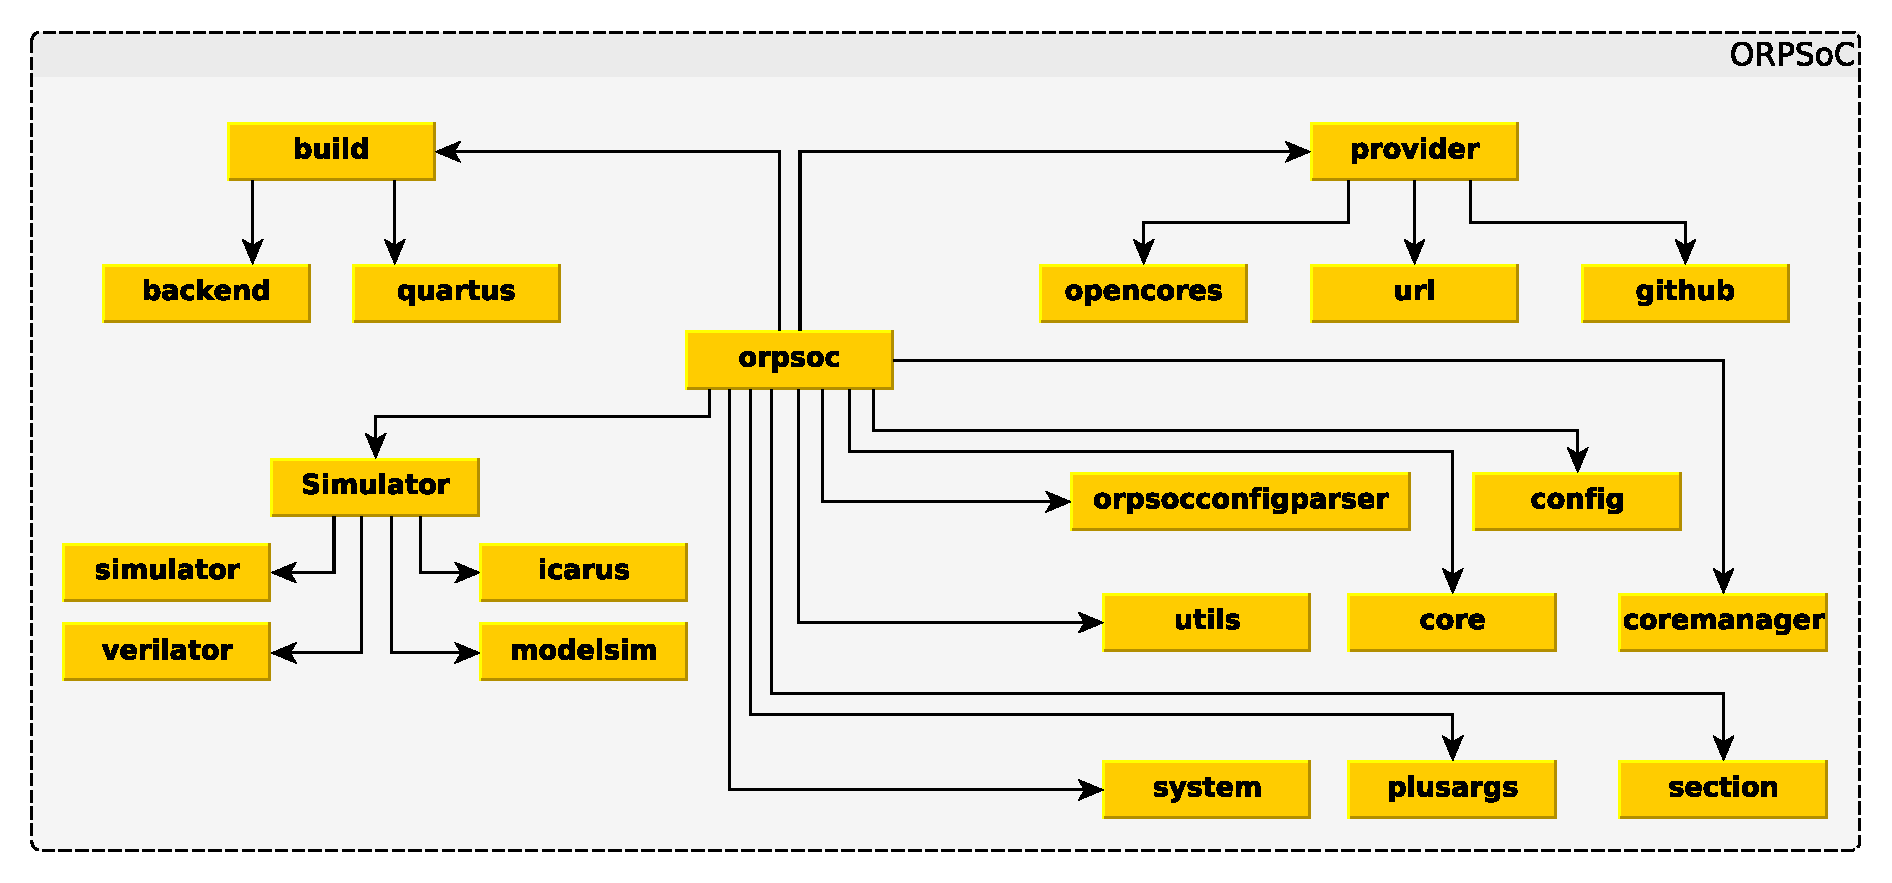
\includegraphics[width=1.00\textwidth]{grafos/Fusesoc.pdf}
  \caption[Diagrama de ficheiros do ORPSoC]{Diagrama de ficheiros do ORPSoC.}
  \label{grafos:fusesoc}
\end{figure}

Durante o desenvolvimento desta tese a comunidade OpenRisc ponderou que esta ferramenta poderia ser utilizada no desenvolvimento de outros \acrshort{soc} sem ser especificamente os seus sistemas. Então a ferramenta tornou-se independente da comunidade e alteram o seu nome para FuseSoC.

\section{Ferramentas}
\label{section:ferramentas}

No desenvolvimento de \acrshort{soc} e de software quando o \acrshort{soc} ainda não se encontra fisicamente criado, é importante ter disponível várias ferramentas de desenvolvimento pois tornasse bastante dispendioso e demorado criar um \acrshort{soc} para desenvolver.

\subsection{Or1ksim}
\label{subs:or1ksim}
% http://opencores.org/or1k/Or1ksim
% http://www.embecosm.com/appnotes/ean1/ean1-tlm2-or1ksim-2.0.html#id2832929

Trata-se de um simulador de um simples \acrshort{soc} da arquitectara OpenRisc 1000, este é desenvolvido em C. Pretende-se que sejas autônomo, que permita umas simulação rápida permitindo analisar o código e avaliação de desempenho do \acrshort{soc}, que seja de fácil configuração de diferentes ambientes alterando o processador, alteração do tamanho das memorias e adicionando novos periféricos e permitir a utilização do debugger remoto. Porem tem a desvantagem do que se está a simular não ser exatamente o que se tem no sistemas descrito e implica quando se faz uma alteração no \acrshort{soc} esta alteração tenha de ser feita também no or1ksim. Mas é optimo para testar código em desenvolvimento por ser bastante rápido a executar. 

\subsection{Verilator}
\label{subs:verilator}

% http://en.wikipedia.org/wiki/Verilator
% http://www.veripool.org/wiki/verilator

O verilator é uma ferramenta que converte o código que descreve o \acrshort{soc} em verilog e converte para objectos em C++ ou systemC. Esses objectos necessitam de ser linkados à testbench que pode ser escrita em C ou systemC. A testbench controla o sinal de clock, podendo também excitar os sinais de entrada e efectuar leitura tando nos sinais de saída como em qualquer final dentro do \acrshort{soc}, como pode ser visto na figura \ref{fig:verilator}. O Verilator é um simulador de dois estados (0,1), é bastante mais lento que o \ref{subs:or1ksim} mas pode disponibilizar um ficheiro que permite visualizar o estado de todos os sinal do \acrshort{soc} a todos os instante da simulação, permitindo assim encontrar erros no hardware. Como é efectuado uma conversam do \acrshort{soc} a simulação efetuada é sobre o \acrshort{soc} desenvolvido.

\begin{figure}[!htb]
  \centering
  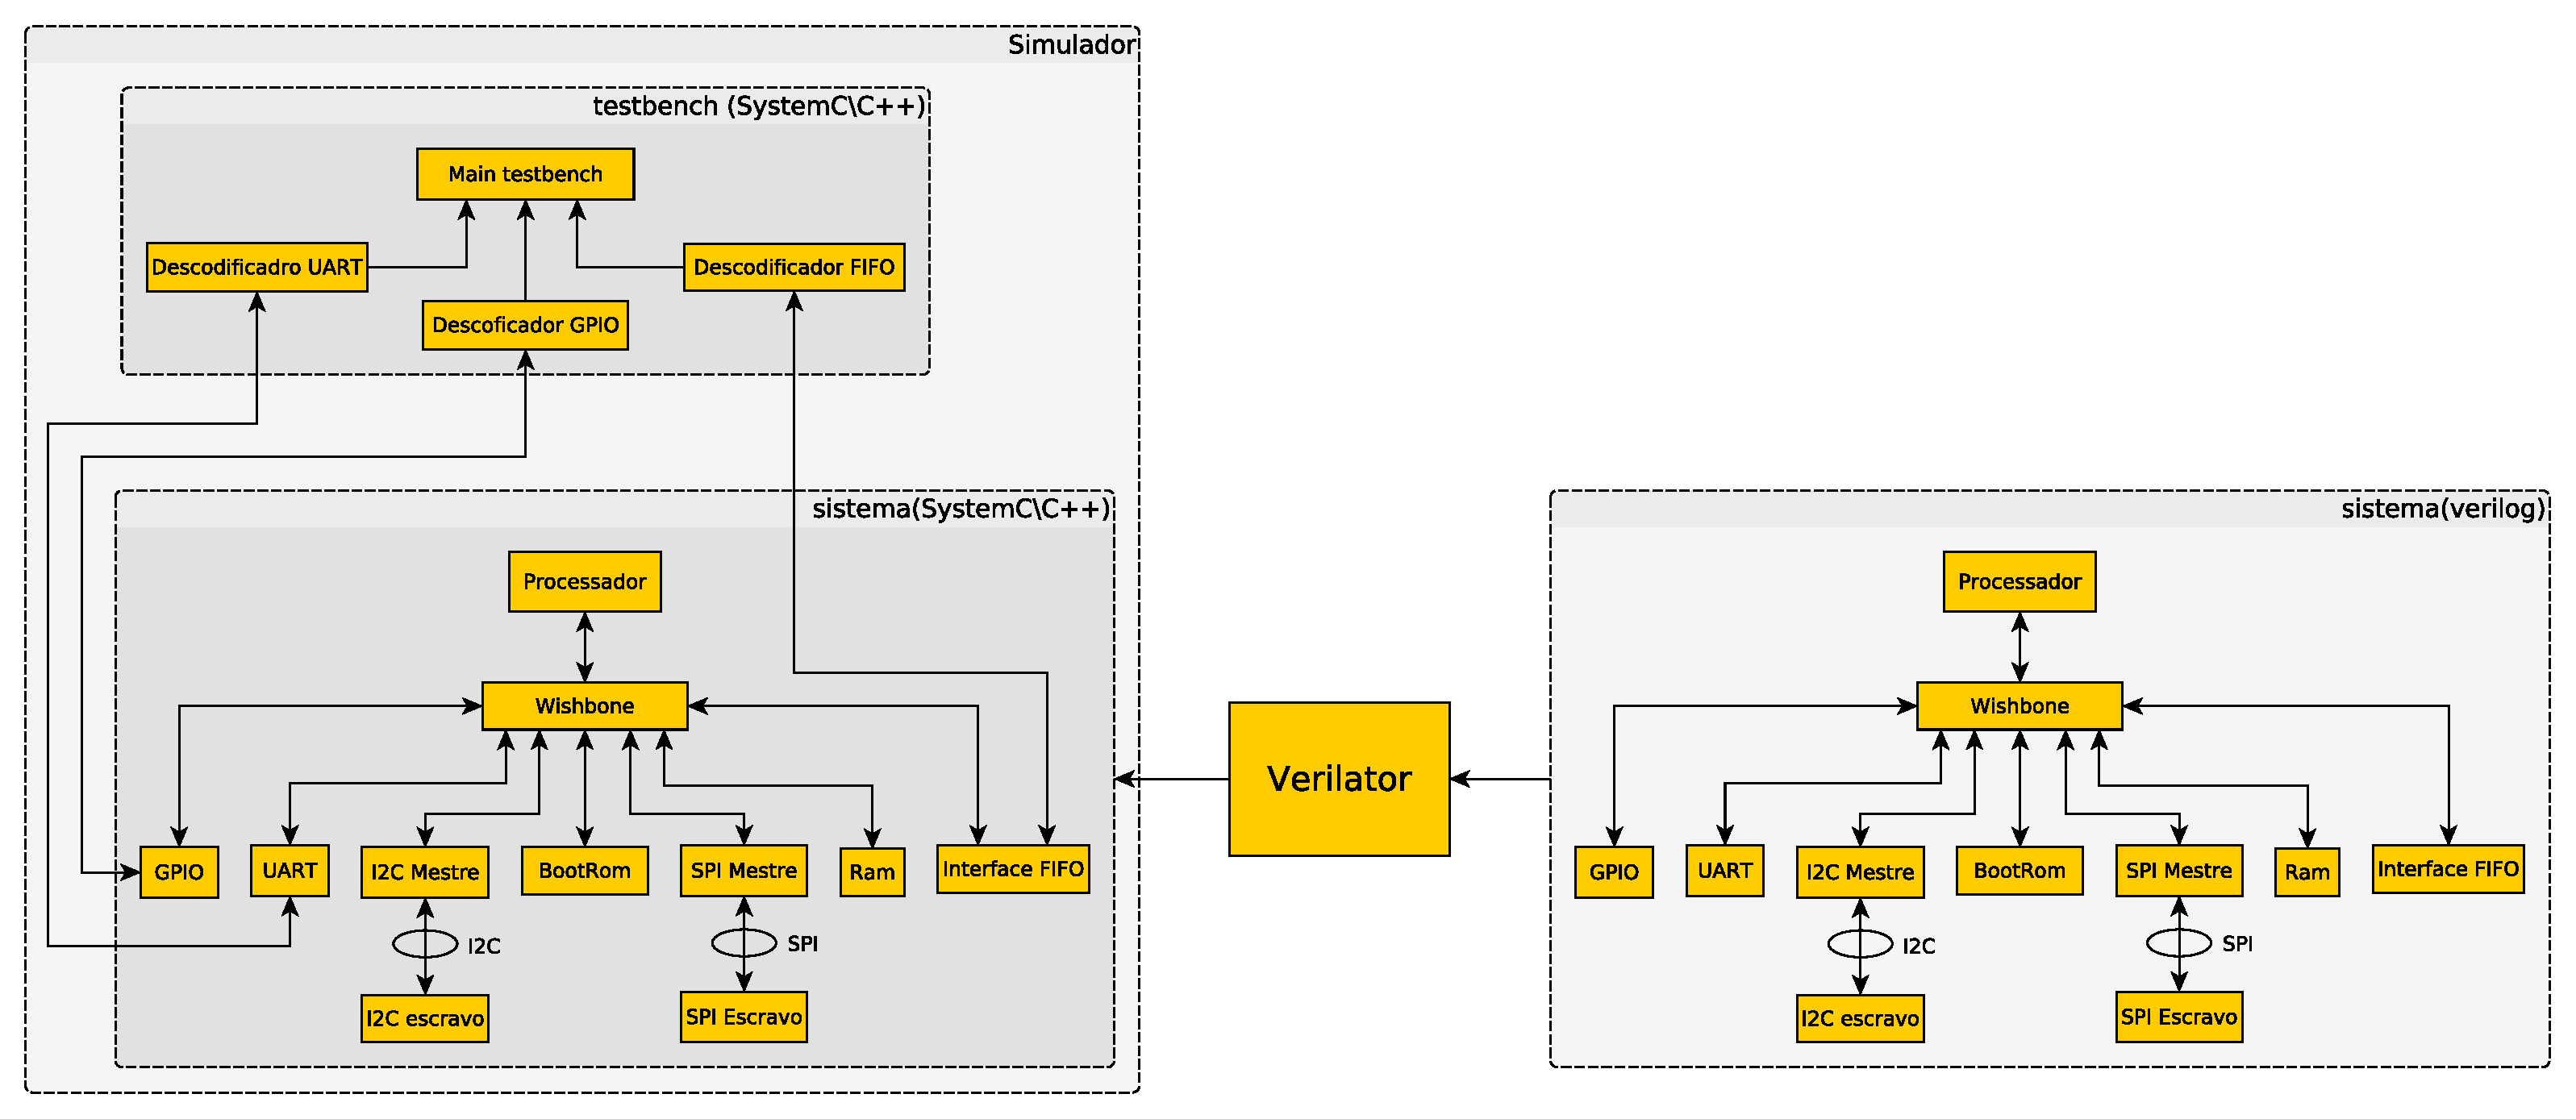
\includegraphics[width=1.00\textwidth]{grafos/Verilator.pdf}
  \caption[Diagrama do simulador verilator]{Diagrama do simulador verilator.}
  \label{fig:verilator}
\end{figure}

\subsection{Icarus}
\label{subs:icarus}

% http://iverilog.icarus.com/
% http://en.wikipedia.org/wiki/Icarus_Verilog
Icarus Verilog conhecido por apenas Icarus é uma ferramenta de simulação e de sintetização de verilog. Funciona como um compilador, compila o codigo fonte me verilog na norma(IEEE-1364) e executa a simulação. Como de pode perceber pela figura \ref{fig:icarus} tal como o \ref{subs:verilator} também necessita de um testbench mas este em verilog. O Icarus é um simulador de três estado, alem dos dois valores lógicos (0,1) também simula o estado de alta impedância, sendo ainda mais próximo da realidade, tal como o \ref{subs:verilator} também disponibiliza o ficheiro do estado dos sinais do \acrshort{soc}. Mas o simulador Icarus é bastante mais lento que o \ref{subs:verilator}.



\begin{figure}[!htb]
  \centering
  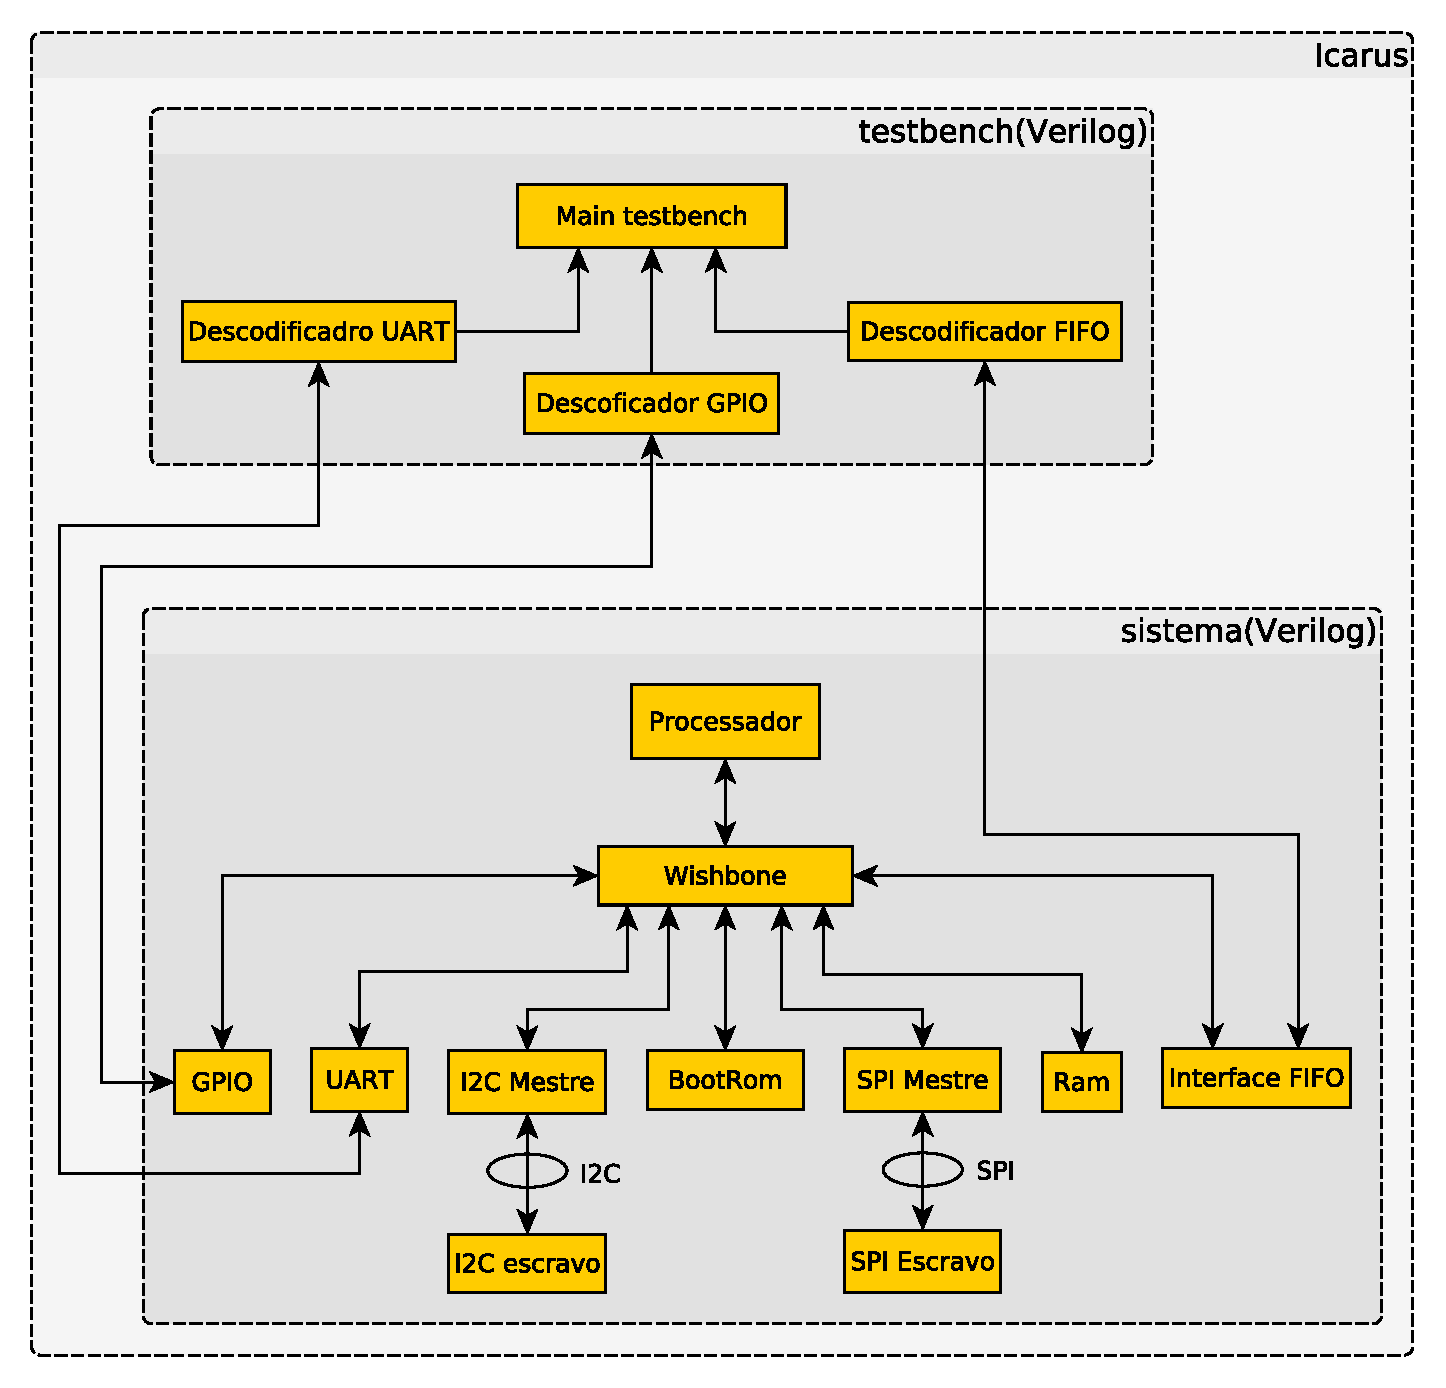
\includegraphics[width=0.75\textwidth]{grafos/Icarus.pdf}
  \caption[Diagrama do simulador icarus]{Diagrama do simulador icarus.}
  \label{fig:icarus}
\end{figure}

\subsection{Placa com processador FPGA}

% http://www.xilinx.com/training/fpga/fpga-field-programmable-gate-array.htm
% http://www.altera.com/products/fpga.html
O processadores \acrlong{fpga} são dispositivos semicondutores que são baseados numa matriz de blocos lógicos configurável. As \acrshort{fpga} podem ser reprogramáveis após a fabricação para requisitos e funcionalidade distintas. permitindo programar recursos e funções, adaptar-se a novas normas, e reconfigurar hardware, mesmo depois do procuro estar aplicado instalado no local.

% http://web.archive.org/web/20050212155202/http://filebox.vt.edu/users/tmagin/history.htm
O primeiro dispositivo lógico programável foi a memória \textcolor[rgb]{1,0,0}{PROM(Programmable read only memory)} sendo tanto programável na fabricação ou pelo utilizador, de onde evoluído o chip \acrshort{fpga}. Em 1985 a Xilinx desenvolve o primeiro chip em que é possível programar os blocos de logica como a interligação entre elas. Em 1987 foi proposto uma ideia de criar um novo chip que utilizava uma nova tecnologia de matrizes de blocos programáveis usando software. a experiencia tinha 2 objetivos determinar uma forma de interligar os planos de matrizes e desenvolver um compilador capaz de programar funções para este chip.

Como foi descrito em cima e se pode ver na figura \ref{fig:PlacaFPGA} o sintetizador é utilizado como um compilador que com toda a descrição do hardware converte essa descrição em um ficheiro de programação para essa \acrshort{fpga}. Para se programar a \acrshort{fpga} é utilizado um software disponibilizado pela marca da \acrshort{fpga}. Assim que é programado o hardware começa em funcionamento. Com um processador \acrshort{fpga} o hardware que estamos a testar é igual não existindo qualquer tipo diferença no código da descrição de hardware para desenvolver o hardware fisicamente, é o mais rápido dos simuladores mesmo que o próprio \ref{subs:or1ksim}, não tem a possibilidade de se visualizar o estado dos sinais. Comparando com os outros sistemas de simulação descritos em cima \ref{subs:or1ksim}, \ref{subs:verilator}, \ref{subs:icarus} utilizar uma placa de \acrshort{fpga} seria o ideal sendo o mais rápido e o mais semelhante em hardware, mas tem o se não é bastante caro comprar uma placa de \acrshort{fpga}. Então utiliza-se cada uma destas ferramenta em situações diferentes o \ref{subs:or1ksim} para o desenvolvimento de software, \ref{subs:verilator} para testar o hardware e resolver alguns problema perspetiveis sem alta impedância, \ref{subs:icarus} para testar o hardware quando não é detectável com o \ref{subs:verilator}, e a placa de \acrshort{fpga} para testar o hardware quando não é detectável com o \ref{subs:icarus} e os testes finais para se certificar o correcto funcionamento do do hardware com o software. 

\begin{figure}[!htb]
  \centering
  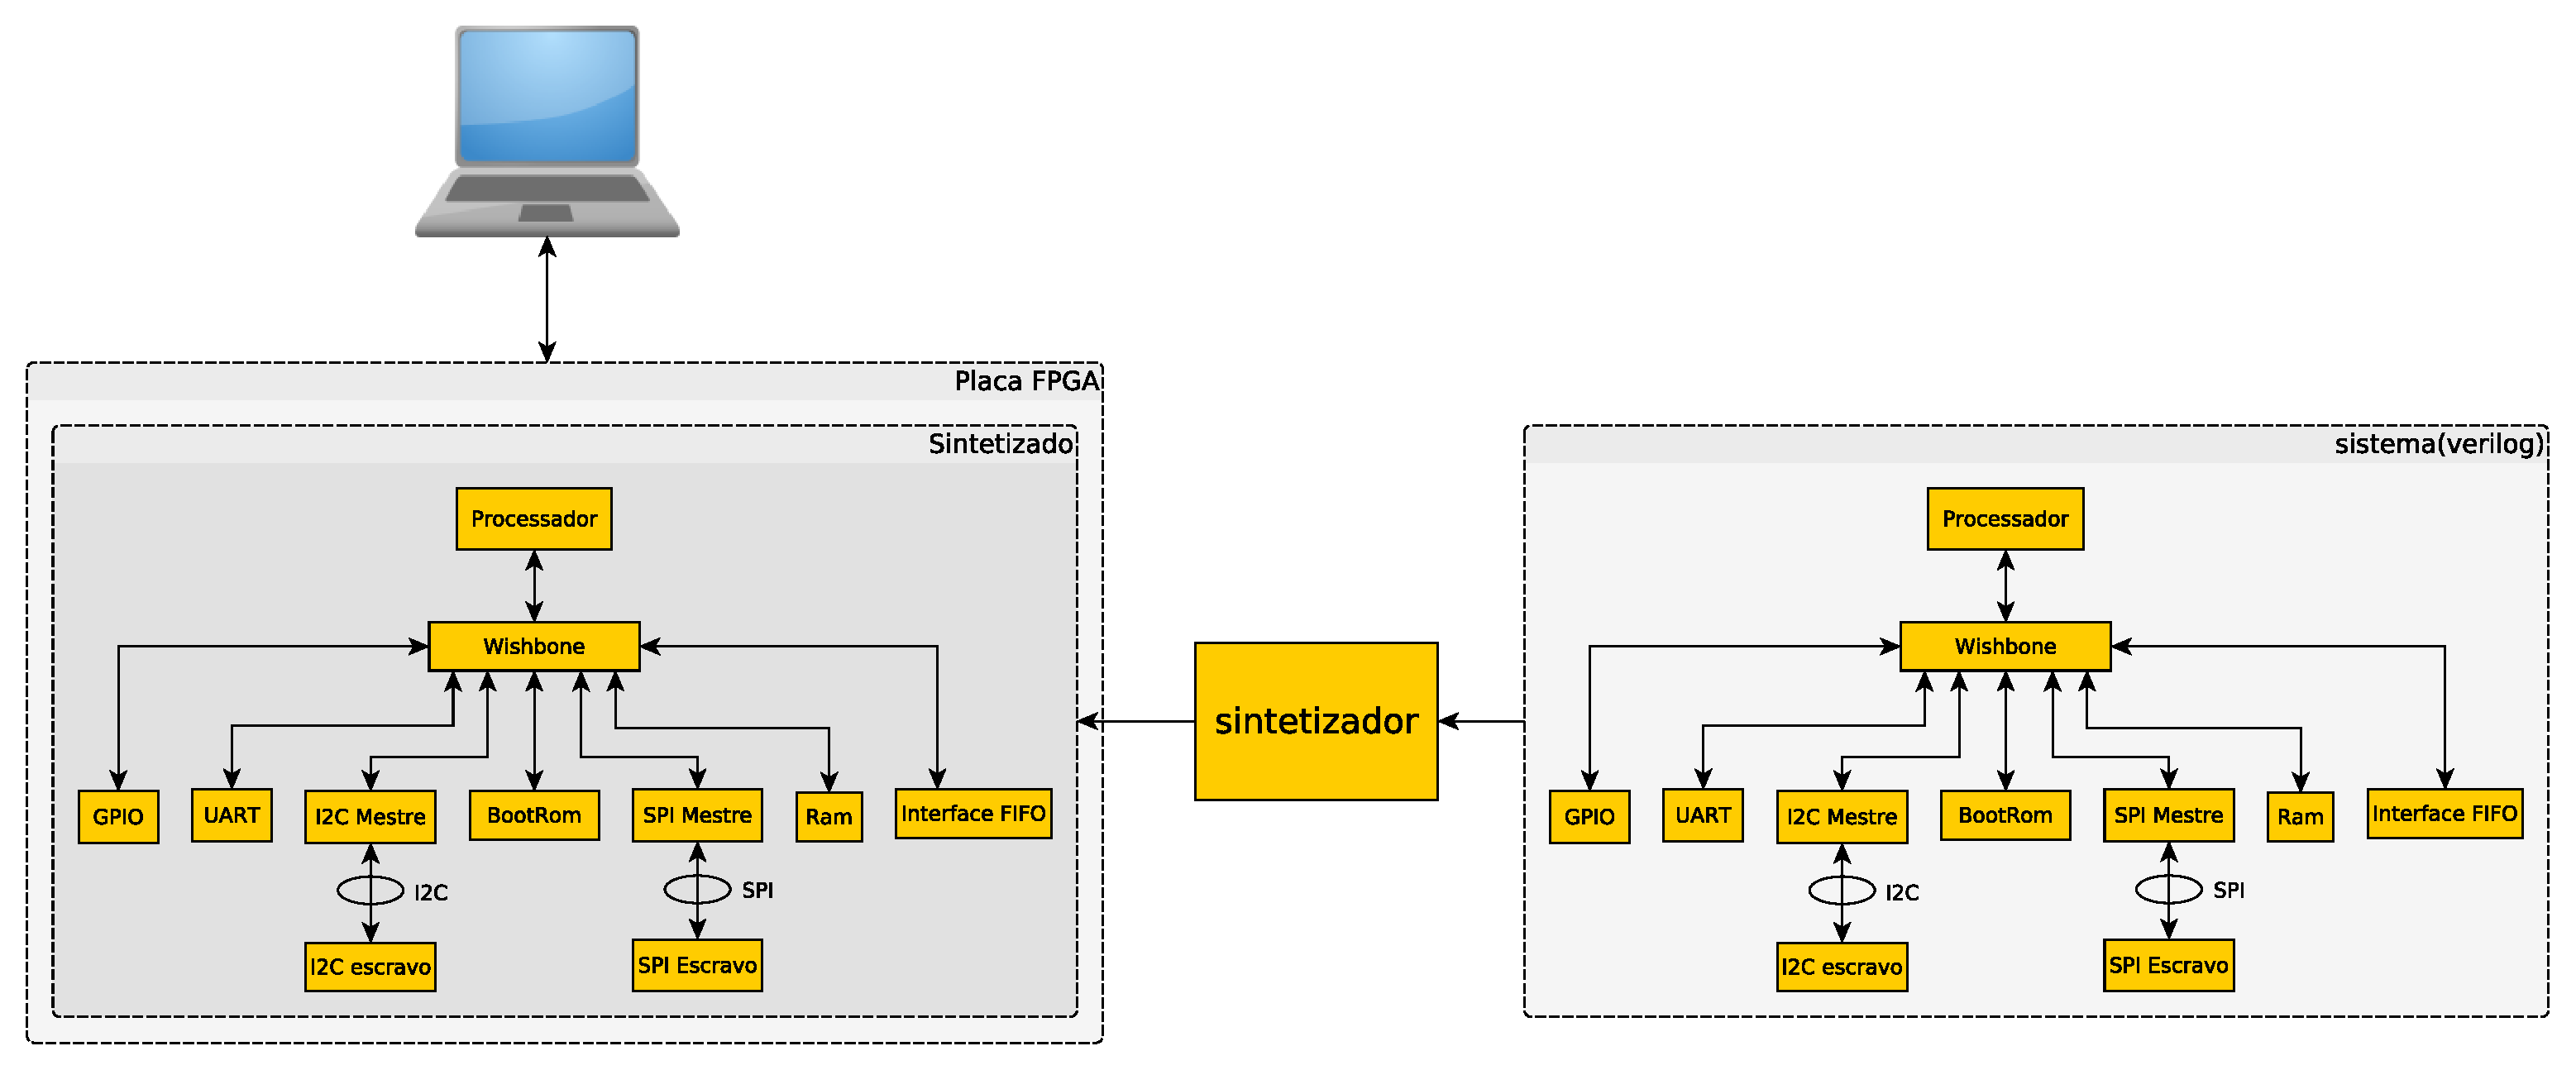
\includegraphics[width=1.00\textwidth]{grafos/FPGA.pdf}
  \caption[Diagrama do funcionamento da placa de FPGA]{Diagrama do funcionamento da placa de FPGA.}
  \label{fig:PlacaFPGA}
\end{figure}

\subsection{OpenOCD}
\label{section:OpenOCD}

% pdf
%http://openocd.sourceforge.net
O \acrlong{openocd} começou inicialmente por uma tese de mestrado onde se pretendia desenvolver e implementar uma solução de debugger para sistemas embebidos baseado na família ARM7 e ARM9. Atualmente existe uma comunidade a trabalhar no \acrshort{openocd} suportando novos \acrshort{soc}, adaptadores de debugger e flash programáveis. O \acrshort{openocd} tem como objectivo disponibilizar debugger, programação em sistemas e testes boundary-scan para dispositivos embebidos. Para isso o \acrshort{openocd} necessita dum adaptadores de debugger alguns deles já se encontram integrados nos dispositivos de desenvolvimentos, não existindo uma uniformização nem por essa razão é possível encontrar de vários tipos, \acrshort{jtag} entre outros, muito delas já com suporte.

Sem utilizar o \acrshort{openocd} tinha-se de desenvolver uma testbench onde se tinha de incluir um servidor de \acrlong{rsp} que estaria ligado por \acrshort{jtag} ao \acrshort{soc}, e disponha de uma ligação com o protocolo TCP/IP para ligar um o cliente de debugger para se efetuar o debuguer. No arranque do \acrshort{openocd} é necessário identificar qual é a placa alvo e qual é a placa de interface que é utilizada para comunicar com a placa. Depois de se iniciar ficar disponível para ligação em tres portos cada um para o ser protocolo como se pode ver na figura \ref{fig:openocd}, e ligando-se a placa de interface por \acrshort{usb}. Vai processando as instruções que vai recebendo conforme o seu alvo e a placa de interface. Enviando-as por \acrshort{usb} para a placa de interface que converte a informação recebida no procolo de comunicação neste caso \acrshort{jtag}, que é recebido pelo \acrshort{soc} pelo seu modelo de \acrshort{jtag} que acaba por enviar para o modelo de \acrshort{ads}. Assim o \acrshort{soc} não necessita de uma testbench onde estaria disponivel o servidor de \acrshort{rsp}, o que este faria é feito pelo o \acrshort{openocd}.

\begin{figure}[!htb]
  \centering
  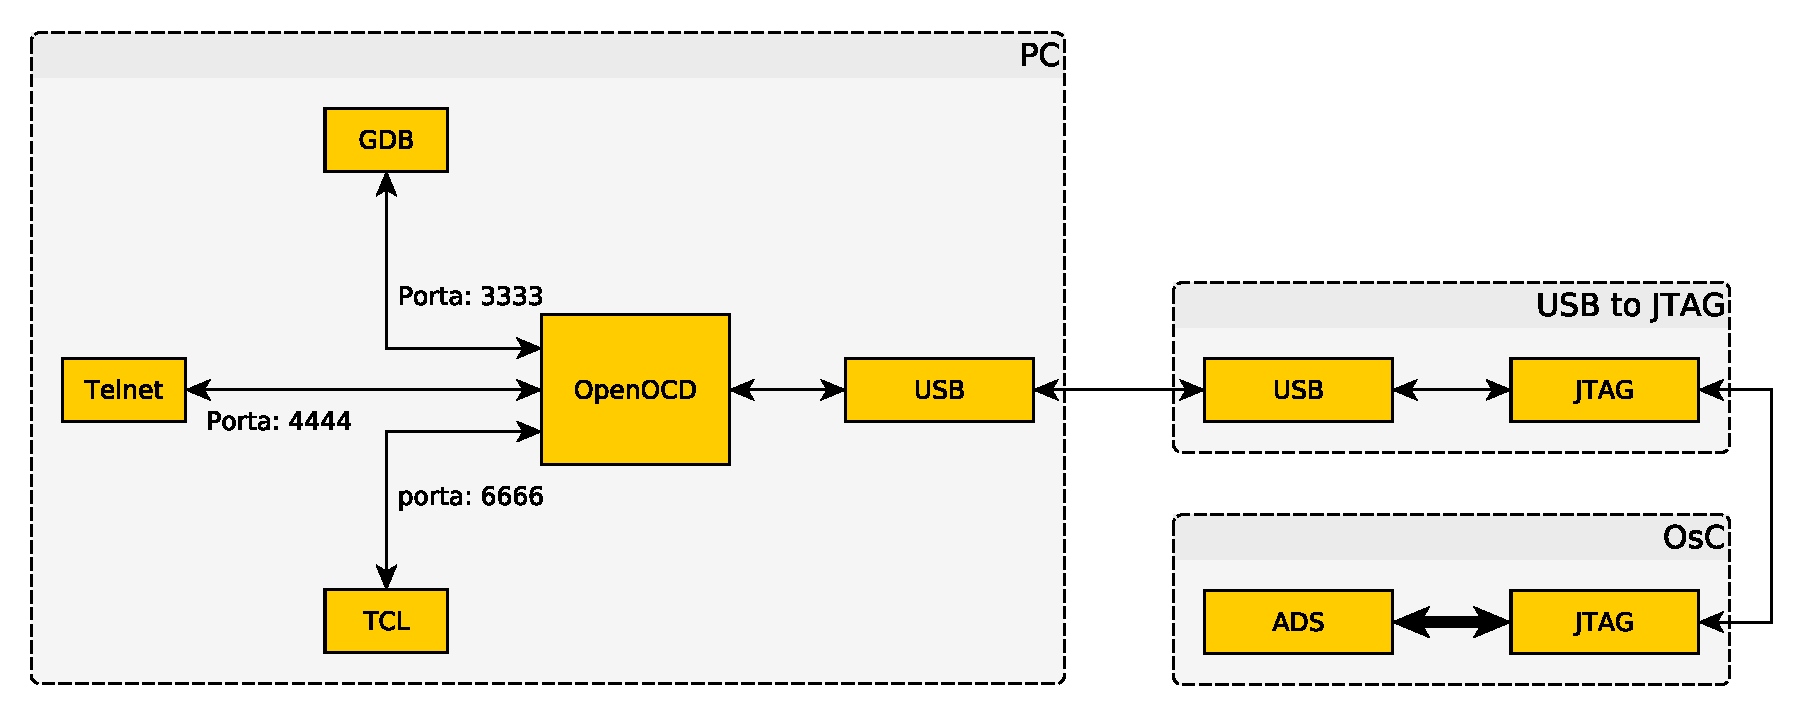
\includegraphics[width=0.75\textwidth]{grafos/openocd.pdf} %1
  \caption[Diagrama do OpenOCD]{Diagrama do OpenOCD.}
  \label{fig:openocd}
\end{figure}

\section{Periféricos}
\label{section:perifericos}

Os Periféricos são modelos com funcionalidades especificas que são acrescidas ao processador, estes comunicam utilizando um barramentos de comunicação neste caso a comunidade utiliza o barramento \ref{section:wishbone}. Os periféricos são conectados ao barramentos como se pode ver na figura \ref{grafos:wishbone}.

\subsection{Bootrom}

A bootrom é uma pequena memoria que tem um rutina de inicialização de sistema. A bootrom pode ser mais ou menos complexa podendo ser como por exemplo um \acrlong{bios} de com computador ou um simples rotina que carregar o programa de uma memoria secundária para a memoria principal(RAM).

\subsection{Uart}
% http://en.wikipedia.org/wiki/Universal_asynchronous_receiver/transmitter
% http://www.societyofrobots.com/microcontroller_uart.shtml

A \acrshort{uart} é um modelo de comunicação assíncrono, o formato dos dados e a velocidade de transmissão de dados são configuráveis. Este normalmente fazem parte de um circuito integrado para comunicação série com computadores ou dispositivos com porta série. O modelo de \acrshort{uart} emissor recebe bytes de dados que os transmite sequencialmente cada bit, o modelo de \acrshort{uart} receptor recebe bit sequenciais e agrupa-os numa byte. A comunicação pode ser simples em que cada modelo só pode fazer apenas de emissor ou receptor, Full duplex em que ambos os modelos podem receber dados ao mesmo tempo e half duplex em que os dois modelos podes receber e enviar mas intercalador.

Por motivos históricos a tinha encontra-se com o valor lógico '1' quando não se encontra uma comunicação a decorrer para mostrar que a linha não foi danificada. Como se pode ver na Figura \ref{fig:uart}, para o caso de envio de 8 bits, o emissor envia inicialmente um bit com valor lógico '0' para informação ao receptor que vai receber um conjunto de bits que pode ser configurável ente 5 a 9 bits, tipicamente é usado 8 bits, seguido sendo opcional de um bit de paridade, se não forem enviados 9 bits, por fim o bit de paragem que tem o valor lógico '1'. Existem vários modelos de chips \acrshort{uart} sendo que a comunidade optou por utilizar no seu \acrshort{soc} a uart16550. O parametros bastante importante é o \textit{Baud rate} ou seja a taxa de transferência o emissor e o receptor tem de estar em acordo se não a transferência não trabalhará corretamente.

Cada modelo de uart é feita por duas linhas TX linha de transmissão e RX linha recepção, a ligação entre os dois modelos é cruzado, ou seja liga-se a linha de TX do primeiro modelo ou RX do segundo modelo e o Tx do segundo modelo ou RX do primeiro modelo.

\begin{figure}[!htb]
  \centering
  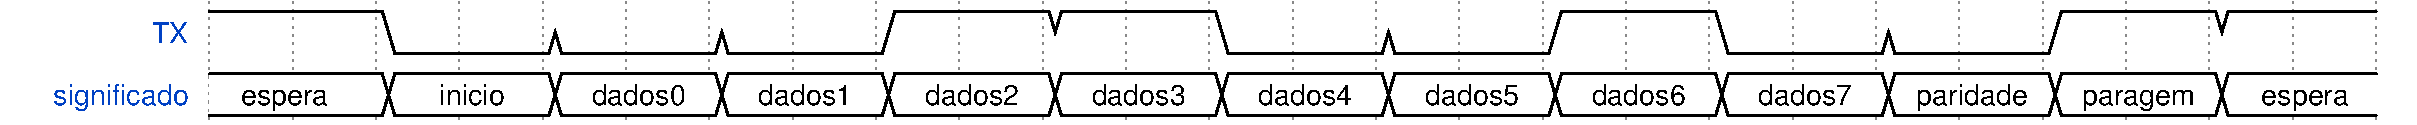
\includegraphics[width=0.75\textwidth]{ondas/uart.pdf} %1
  \caption[Diagrama temporal da UART]{Diagrama temporal da UART}
  \label{fig:uart}
\end{figure}

\subsection{GPIO}

O \acrlong{gpio} como o nome indica trata-se um de pinos de input e output de uso genérico, este pinos não têm uma função especifica. São apenas linhas disponíveis e controladas pelo utilizador em tempo de execução. A ideia é na construção de um \acrshort{soc} pode dar jeito ter disponível linhas de controlo digital e não necessitar de ter de organizar o chip por forma em as conseguir. Os pinos de \acrshort{gpio} podem ser activos ou desactivos, permitindo serem programados como input ou output. Os pinos que estão configurados por input permitem apenas leituras, normalmente de valores lógicos '0' ou '1', estes ainda por vezes são utilizados para criar interrupções no processador. Os pinos em output permitem leituras e escritas.

Os GPIO tem algumas aplicações tipicas como \acrshort{soc} pelas sua escassez de pinos disponíveis, portas multifunções como em gestão de energia, codecs de audio e placas de video e por aplicações em sistemas embebidos para comunicação com sensores, LCD's, LED's para estados. Alguns exemplos mais práticos dos pinos \acrshort{gpio} são alguns computadores portáteis da ACER usar o GPIO0 para ligar o amplificar da colunas internas, o chip Realtek ALC260 tem disponivel 8 pinos de GPIO que não são utilizados por omissão.


\subsection{FIFO}

A interface \acrlong{fifo} destina-se a interligar um modelo assíncrono ao \acrshort{soc} com comunicação paralela de 32 bits por palavra, queria-se com esta interface que a comunicação seja rápida entre os dois modelos. Para uma comunicação paralelas com modelos assíncronos é utilizada uma memoria do tipo \acrshort{fifo} para cada sentido, ou seja uma \acrshort{fifo} para o \acrshort{soc} escrever e o modelo ler e outra para o oposto. Estas \acrshort{fifo}'s ficaram ligadas a interface que \ref{section:wishbone} permitindo uma rápida comunicação com o processador. Para alem disso será possível efetuar ligação da \acrshort{fifo} de recepção ao interrupções, permitindo assim efetuar uma sub-rotina de interrupção permitindo assim que a resposta do processador seja mais ainda mais rápida e que se possa por em modos de poupança de energia.

\subsection{I2C}

%pdf xnp e phiçips
% http://en.wikipedia.org/wiki/I%C2%B2C

O \acrlong{i2c} é um barramento desenvolvido pela Philips semicondutores agora conhecida como NXP semicondutores, é uma barramento serie, síncrono, multi-mestres, multi-escravos. Desenvolvido para conectar periféricos de baixa velocidade a computadores, sistemas embebidos e a telefones celulares. Este barramento utiliza apenas duas linhas de comunicação \acrlong{sda} para o envio de dados e \acrlong{scl} sinal de clock que é controlado pelo o mestre, estas duas linhas são de dreno aberto. O \acrshort{i2c} define tipo simples de comunicação o mestre lé dados do escravo, o mestre escreve dados para o escravo e combinado onde o mestre faz pelo menos duas leituras e/ou escritas, estas comunicação começam sempre por um sinal de começo(START) e acabando por um sinal de paragem(STOP). Todos os escravos têm um endereço de identificação, que é utilizado para diferencias com qual dos escravos o mestre quer comunicar.

%pdf philips
Este barramento desde de Outubro de 2006 não necessita de licenciamento para ser utilizado. Tendo cada vez mais utilizações praticas como acesos a pequenas memorias de sistemas embebidos, comunicação com conversores digitai para analógico e analógico para digital, controlo pequeno monitores como para telemóveis são alguns dos exemplos.


\subsection{SPI}
\label{section:spi}

O \acrlong{spi} é um barramento serie, síncrono, que permite apenas um único mestres e opera em \textit{full-duplex}(ou seja permite receber e enviar dados ao mesmo tempo). O barramento utiliza pelo menos 4 linhas, isto porque necessita de uma linha para cada escravo, utiliza uma linha de clock comum a todos os escravos \acrlong{sclk}, tem duas linhas para dados uma que envia do mestre para o escravo \acrlong{mosi} e outra que envia dados do escravo para o mestre \acrlong{miso}, por ultimo tem a linha que seleciona o escravo com que se encontra a comunicar \acrlong{ss} existem tantas linhas deste tipo no mestre como escravo estão ligados ao barramento sendo cada linha para cada escravo, esta linha é \textit{active low} significa que o escravo só se encontra selecionado quando este linha se encontra num valor lógico '0'. Este barramento é utilizado para pequenas distancia em que o tempo é importante, como sistemas embebidos, sensores, lentes da Canon, LCD cartões SD.

ve se queres por aqui mais coisas.



 % file "Thesis_Estado_da_arte.tex"

%%%%%%%%%%%%%%%%%%%%%%%%%%%%%%%%%%%%%%%%%%%%%%%%%%%%%%%%%%%%%%%%%%%%%%%%
%                                                                      %
%     File: Thesis_SPI.tex                        %
%     Tex Master: Thesis.tex                                %
%                                                                      %
%     Author: Carlos A. Rodrigues                         %
%     Last modified : 15 Abril 2013                         %
%                                                                      %
%%%%%%%%%%%%%%%%%%%%%%%%%%%%%%%%%%%%%%%%%%%%%%%%%%%%%%%%%%%%%%%%%%%%%%%

\chapter{SPI}
\label{chapter:spi}

% pdf sd_spi
O nosso \acrshort{soc} tem disponível uma memoria principal voatil ou seja sempre que a memoria é desligada da fonte de alimentação perde a informação contida nela. Então é necessário ter disponível no \acrshort{soc} uma outra memoria que não seja voatil como um cartão \acrlong{sd}, uma EEPROM, para se poder guardar o programa, que será carregado para a memoria principal sempre que o \acrshort{soc} for inicializado ou seja alimentado. Optou-se pela utilização de um cartão \acrshort{sd} por permitir uma fácil substituição em qualquer local que esteja aplicado o \acrshort{soc} a trabalhar, estando planeado que estagia a trabalhar em locais de difíceis acessos. O cartão \acrshort{sd} é possível ligar-se por barramento \acrshort{spi}, como se pode ver na tabela \ref{table:pin_sd_card} e a correspondência entre os pinos na figura \ref{fig:cartao_SD} que se encontra ao lado.

\textcolor[rgb]{1,0,0}{melhorar a posição disto}

  \begin{minipage}{\textwidth}
  \begin{minipage}[b]{0.20\textwidth}
    \centering
    \includegraphics[width=1\textwidth]{Figures/sd_card.pdf}
    \captionof{figure}{Cartao SD}
    \label{fig:cartao_SD}
  \end{minipage}
  \hfill
  \begin{minipage}[b]{0.99 \textwidth}
    \centering
    \begin{tabular}{c | c | c| c}\hline
      Pinos SD & Nome(SD) & Nome (SPI) & Descrição  \\ \hline
        1 & CS & SS & Selectiona o cartão \\
        2 & DI & MOSI & Entrada de dados\\
        3 & VSS & -- & Tensão de alimentação(massa) \\
        4 & VDD & -- & Tensão de alimentação \\
        5 & SCLK & SCLK & Clock \\
        6 & VSS & -- & Tensão de alimentação(massa) \\
        7 & DO & MISO & Saida de dados\\
        8 & RSV & -- & Reservado  \\
        9 & RSV & -- & Reservado \\ \hline
      \end{tabular}
      \captionof{table}{Relação pinos do cartão SD SPI}
      \label{table:pin_sd_card}
    \end{minipage}
  \end{minipage}

Como foi dito \ref{section:spi} o \acrshort{spi} é um barramento de comunicação utilizado em casos onde é necessário uma comunicação com a velocidade de transferências elevada, como é neste caso. O barramento é constituído por 3 linhas de comunicação mais uma por cada escravo que esteja ligado a mestre como se pode ver na figura \ref{fig:ligacoesSPI}, neste caso como tem três escravos têm 3 linhas mais 3 linhas de selecção de escravo. A linha que seleciona o escravo é a linha \acrshort{ss} esta é seleciona o escravo quando tem um valor lógico de '0'. Apenas o escravo que está selecionado lé e/ou escreve no barramento, como se trata de barramento full-duplex têm disponível uma linha de leitura para o escravo \acrshort{mosi}  e outra de escrita do escravo \acrshort{miso}. Ainda existe mais uma linha de sincronização com um sinal de clock \acrshort{sclk}. Todas as linhas do barramentos com as excepção da \acrshort{ss} são partilhadas por todos os escravos, a linha \acrshort{ss} como se trata de uma linha de selecção de escravo cada escravo tem a sua linha independente. Para se efetuar comunicação o mestre SPI seleciona com qual escravo quer comunicar, dependendo do escravo com que está a comunicar enviar uma ou mais palavras de 8 bits na linha \acrshort{mosi} sincronizado com o sinal de clock que se encontra na linha \acrshort{sclk}, posteriormente o mestre necessita de transmitir mais sinais de clock para o escravo, para este poder transmitir os dados pedidos pelos mestres na linha \acrshort{miso}.

\begin{figure}[!htb]
  \centering
  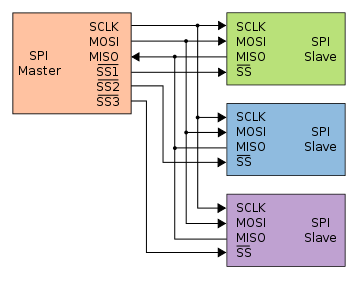
\includegraphics[width=0.50\textwidth]{Figures/SPI.png}
  \caption[Protocolo SPI]{Esquematico do sistema de comunicação SPI, com 1 master e vários escravos"tirou do wiki".}
  \label{fig:ligacoesSPI}
\end{figure}

\section{Mestre SPI}

A comunidade OpenRISC já tinha disponível um core de mestre \acrshort{spi} com uma interface Wishbone disponível para ligação ao \acrshort{soc}. Porém este core apenas realizava corretamente escritas para o escravo, não efetuando qualquer leitura de dados enviada pelo escravo. Sendo uma parte indispensável para o objectivo que seria pretendido para o core de \acrshort{spi}, como foi dito em cima seria efetuar leituras de uma memoria de um cartão \acrshort{sd} para efetuar o carregamento do programa para a memoria principal.

Na figura \ref{fig:diagrama_SPI_master} pode ser visto o fluxo de dados dentro do core mestre de SPI. Quando se pretende enviar uma palavra para o escravo esta é recebida pelo cores vindo da interface Wishbone que se encontra ligada ao processador do \acrshort{soc}, é guardada na \acrshort{fifo}, com uma tamanho de 4 palavras, que contem as palavras que serão enviadas para o escravo, na figura tem o nome de \acrshort{fifo} IN. Quando o modelo que faz a serialização se encontra parado e tem disponível uma palavra para enviar na \acrshort{fifo}. O modelo vai buscar a palavra à \acrshort{fifo} e começa a gerar clocks ao mesmo tempo que serializa a palavra e a enviar bit a bit para o escravo pela linha \acrshort{mosi}.

Quando se pretende receber dados do escravo, o modelo de desserialização recebe essa informação e se a \acrshort{fifo} que recebe as palavras vindas do escravo, na figura com o nome de \acrshort{fifo} OUT, não estiver cheia, começa a gerar clock's. O modelo recebe bit a bit a palavra do escravo na linha \acrshort{miso}, quando receber a palavra toda deixa de gerar clocks e enviar a palavra para a \acrshort{fifo}. Em seguida a palavra será enviada da \acrshort{fifo} para o processador pela interface Wishbone. Visto que se trata de um barramento full-duplex quando se encontra a enviar dados para o escravo, o mestre também lé a linha \acrshort{miso} e guarda a palavra da \acrshort{fifo}. No caso destes dados forem lixo é necessário ter em atenção se os dados não forem removidos da \acrshort{fifo} quando se for efectuar a primeira leitura podemos estar a ler lixo. 

\begin{figure}[!htb]
  \centering
  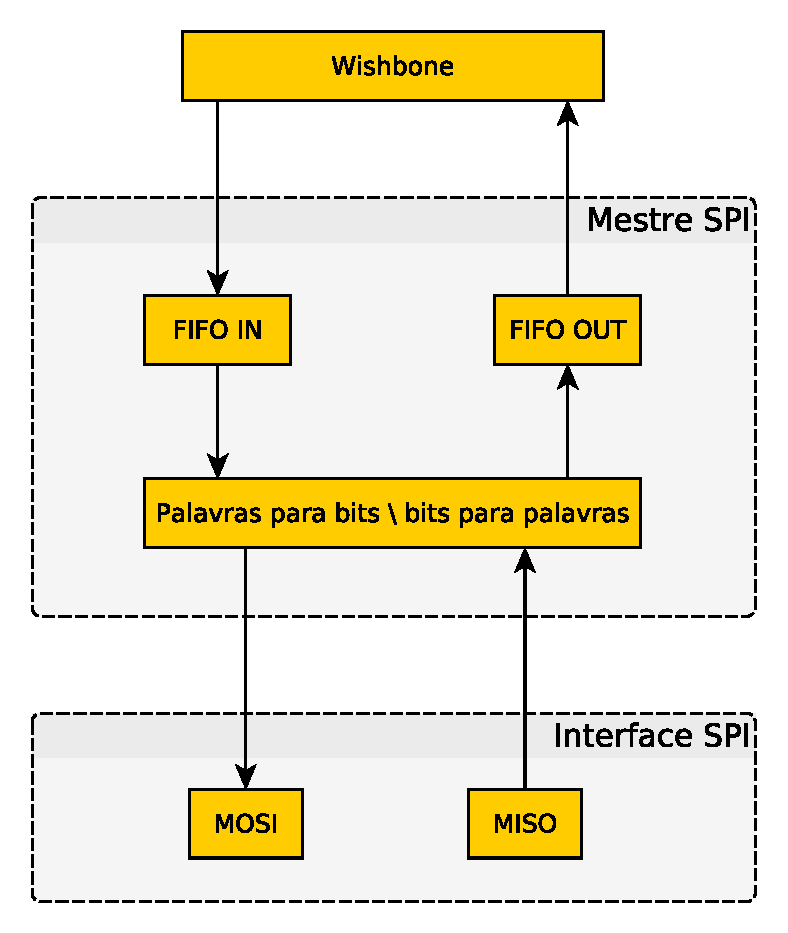
\includegraphics[width=0.50\textwidth]{grafos/diagrama_SPI_master.pdf}
  \caption[Fluxo dos dados dentro do core mestre SPI]{Fluxo dos dados dentro do core mestre SPI}
  \label{fig:diagrama_SPI_master}
\end{figure}

Na tabela \ref{table:sinais_SPI_master} temos todos os sinais do core mester de \acrshort{spi} com uma pequena descrição, os primeiros 10 sinais correspondem à interface Wishbone que é ligado ao multiplexer wishbone de dados á semelhança dos cores de uart e de gpio como se pode ver na figura \ref{grafos:wishbone}. Os ultimos quatros sinais correspondem a barramento \acrshort{spi} para serem ligados ao escravo.

\begin{table}[h!]
  \begin{center}
    \begin{tabular}{|C{2cm}|c|c|c|}
      \hline
       Interface & Nome & direcção & Descrição \\
      \hline \hline
      \multirow{10}{*}{Wishbone} & clk\_i & input & Clock, Recebido pelo Wishbone. \\
      \cline{2-4}
      & rst\_i & input & Reset, renicia o core quando se encontra no valor logic "1".\\
      \cline{2-4}
      & cyc\_i & input & \\
      \cline{2-4}
      & stb\_i & input & \\
      \cline{2-4}
      & adr\_i & input & Endereço do registo onde se pretende ler ou escrever no core.\\
      \cline{2-4}
      & we\_i & input & Bit de selecção de escrita.\\
      \cline{2-4}
      & dat\_i & input & Recepção de dados por parte do processador.\\
      \cline{2-4}
      & dat\_o & output & Envio de dados para o processador.\\
      \cline{2-4}
      & ack\_o & output & bit que informação o processador a recepção do comando pelo core.\\
      \cline{2-4}
      & inta\_o & output & bit de interrupção. \\
      \hline \hline
      \multirow{4}{*}{SPI} & sck\_o & output & Clock do protocolo de comunicação SPI.\\
      \cline{2-4}
      & ss\_o & output & Faz a selecção do escravo que se pretende ler ou escrever.\\
      \cline{2-4}
      & mosi\_o & output & envio de dados para o escravo (master Out Slave In).\\
      \cline{2-4}
      & miso\_i & input & recepecção de dados do escravo (master Out Slave In).\\
      \hline
    \end{tabular}
  \end{center}
  \caption[Tabela de sinais do core SPI master]{Tabela de sinais da interface SPI master}
  \label{table:sinais_SPI_master}
\end{table}

A tabela \ref{table:registos_SPI_master} é uma descrição dos registos do mestre \acrshort{spi} com uma pequena descrição de cada registo e o seu Offset. 

\begin{table}[h!]
  \begin{center}
    \begin{tabular}{|c|c|c|c|}
      \hline
      Nome & leitura/escrita & Descrição & Offset End. \\
      \hline \hline
      Registo de controlo & escrita e leitura &  & 0X00 \\
      \hline
      Tipo de leitura & escrita  & selectiona o tipo de leitura que é pretendida no SPI & 0X01 \\
      \hline
      Registo de estado & leitura & disponibliza várias informações do estado do core & 0X01 \\
      \hline
      Leitura de dados & leitura & leitura dos dados recebidos pelo SPI & 0X02 \\
      \hline
      Escrita de dados & escrita & escrita dos dados a enviar pelo SPI & 0X02 \\
      \hline
      Ext.registo de controlo & escrita e leitura & & 0X03 \\
      \hline
      selecção do escravo & escrita e leitura & seleciona o escravo que se pretende escrever ou ler & 0X04 \\
      \hline
    \end{tabular}
  \end{center}
  \caption[Tabela de registo do core SPI master]{Tabela de registos da interface SPI master}
  \label{table:registos_SPI_master}
\end{table}

O core mestre de \acrshort{spi} disponibiliza o modo de escrita que já se encontrava funcional, ficando a disponibilizar também o modo de leitura de dados que não se encontrava totalmente funcional. Esta leitura que a vou chamar de simples era feita apenas quando o era pedida pela processador ou seja, o processador pedia para ler uma palavra ao core, ai ele realizava a leitura no core. Este tipo de leitura perde-se bastante tempo porque o processador tinha de ficar a espera o core efectua-se a leitura ao escravo e que este o respondesse com a palavra, principalmente se pensarmos para que tipo de funcionalidade foi adicionado, para efetuar leitura sucessivas e posições de memorias sequenciais. Então pensei como poderia diminuir o tempo em que o processador tivesse a espera da resposta do core de forma transparante para ele. A solução encontrada é existir dois modos de leitura, um modo simples descrito em cima e outro modo em brust. Quando se efectua uma leitura é necessário identificar o tipo de leitura ao core, isto é feito no registo com o offset 0x01 como se pode ver na tabela \ref{table:registos_SPI_master} se escrevemos a palavra 0x02 é uma leitura simples, se for 0x01 é uma leitura brust. A principal diferença entre os dois modos de leitura é que o core na leitura simples vai pedir dados escravo após cada pedido pelo processador, na leitura em brust o core faz pedidos de dados sucessivos ao escravos até a \acrshort{fifo} OUT ficar cheia, ou seja não espera que o processador peça dados. Este tipo de leitura só mostra vantagem quando são leitura sucessivas de vários dados sucessivos como por exemplo a carregar o programa na memoria principal, \textcolor[rgb]{0,1,0}{como se pode ver nas figuras XXXX por imagem das ondas a comprar o tempo.}

\section{escravo SPI}

dizer que foi desenhado desde o inicio.

por um diagrama de blocos de como circula a informa\c{c}\~ao dentro do meu modelo de SPI. fazer uma descri\c{c}\~ao do funcionamento com uma descri\c{c}ao do fluxo de dados.
\begin{figure}[!htb]
  \centering
  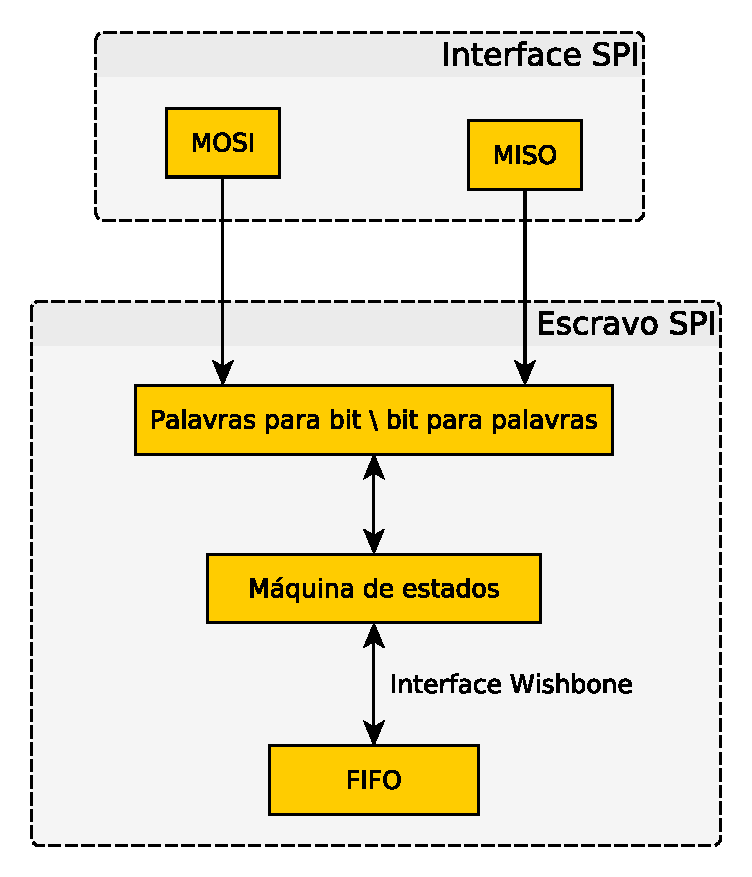
\includegraphics[width=0.50\textwidth]{grafos/diagrama_SPI_slave.pdf}
  \caption[Fluxo de dados dentro do core SPI escravo]{Fluxo dos dados dentro do core SPI escravo}
  \label{fig:diagrama_SPI_slave}
\end{figure}

por a tabela de sinais da interface de SPI (sinais de entrada e saida)
\begin{table}[h!]
  \begin{center}
    \begin{tabular}{|c|c|c|}
      \hline
      Nome & direcção & Descrição \\
      \hline \hline
      clk\_i & input & Clock, Recebido pelo Wishbone. \\
      \hline
      rst\_i & input & Reset, renicia o core quando se encontra no valor logic "1".\\
      \hline
      sck\_o & input & Clock do protocolo de comunicação SPI.\\
      \hline
      ss\_o & input & selectiona se é o escravo pretendido\\
      \hline
      mosi\_o & input & recepecção de dados do master (masterOut SlaveIn).\\
      \hline
      miso\_i & output & envio de dados para o master (masterOut SlaveIn).\\
      \hline
    \end{tabular}
  \end{center}
  \caption[Tabela de sinais SPI escravo]{Tabela de sinais da interface SPI escravo}
  \label{table:sinais_SPI_slave}
\end{table}

explicar o modo de funcionamento de esrita e de leitura.

explicar os 2 modos de funcionamento de esrita e de leitura que tem 2 modos.

\section{Diagramas temporais}

Em seguida temos os diagramas temporais com uma breve explicação do que se encontra em cada diagrama.

\subsection{Selecção de chip}

Na figura \ref{fig:ondas_SPI_S} estão ligados dois escravos ao mestre de \acrshort{spi}, por essa razão existes dois sinais de \acrshort{ss} cada um ligado apenas a uma escravo.
Como foi dito em cima o sinal de \acrshort{ss} é ativo em baixo, significa que o escravo está selecionado quando o seu sinal tem o valor lógico de '0'. No primeiro flanco positivo da figura \ref{fig:ondas_SPI_S} não se encontra qualquer um dos escravos selecionado, o escravo um é selecionado no primeiro flanco negativo e assim se mantem até ao segundo flaco negativo, o segundo escravo é selecionado no terceiro flanco negativo e desselecionado no quarto flanco negativo. Apenas o segundo e o quarto flanco positivo têm um escravo selecionado, o primeiro e o segundo escravo correspondentemente. 

\begin{figure}[!htb]
  \centering
  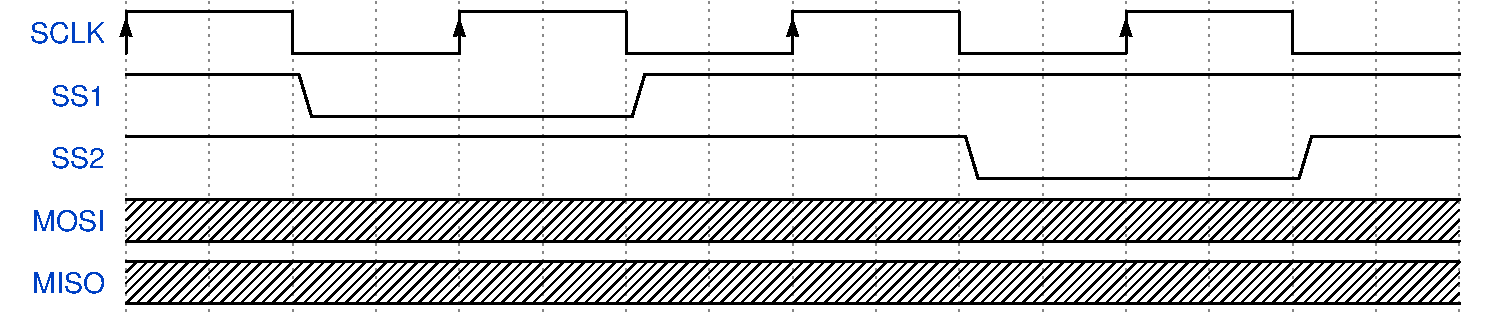
\includegraphics[width=0.75\textwidth]{ondas/SPI_S.pdf} %0.5
  \caption[Diagrama temporal da selecção do escravo.]{Diagrama temporal da selecção do escravo.}
  \label{fig:ondas_SPI_S}
\end{figure}

\subsection{Dados}

Os dados transmitidos tanto pelo mestre ou pelo escravo são lidos nos flancos positivo.

\subsubsection{Envio de dados pelo mestre}

No caso do envio dos dados do mestre para o escravo estes são feitos pelo sinal \acrshort{mosi} como se pode ver na figura \ref{fig:ondas_SPI_Se}. O escravo apenas vai guardar os dados que forem enviados depois de ser selectionado, que so acontece após o segundo flaco positivo. Após o escravo ser selecionado os dados são lidos no flanco positivo do sinal de \acrshort{sclk}, nesta figura por exemplo as palavras são de 6 bits, a palavra recebida pelo escravo no exemplo da figura é 110100 na base binária.

\begin{figure}[!htb]
  \centering
  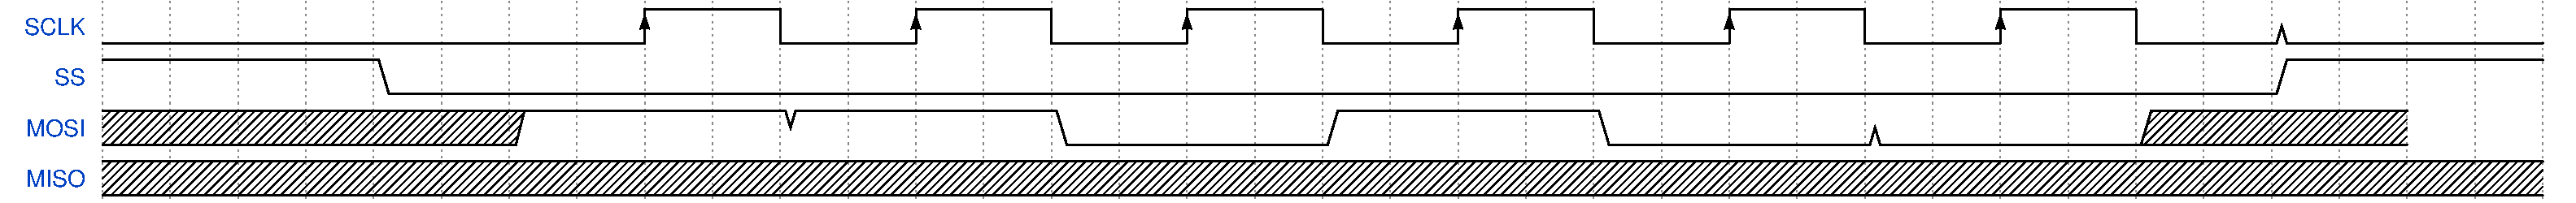
\includegraphics[width=1.00\textwidth]{ondas/SPI_Se.pdf} %0.5
  \caption[Diagrama temporal do envio de dados pelo mestre.]{Diagrama temporal do envio de dados pelo mestre.}
  \label{fig:ondas_SPI_Se}
\end{figure}

\subsubsection{Envio de dados pelo escravo}

Para o escravo enviar dados para o mestre, o mestre necessita de criar o sinal de clock em \acrshort{sclk} e o escravo só pode usar o sinal \acrshort{miso} quando se encontra selecionado. Como no envio de dados do mestre para o escravo, neste caso do envio de dados do escravo para o mestre os dados são lidos nos flancos positivos do sinal de clock gerado pelo mestre. A caso de exemplo a figura \ref{fig:ondas_SPI_Re} a palavra envida pelo escarvo é de apenas 6 bits, neste exemplo a palavra transferida pela o escravo é 010110 na base binária. 

\begin{figure}[!htb]
  \centering
  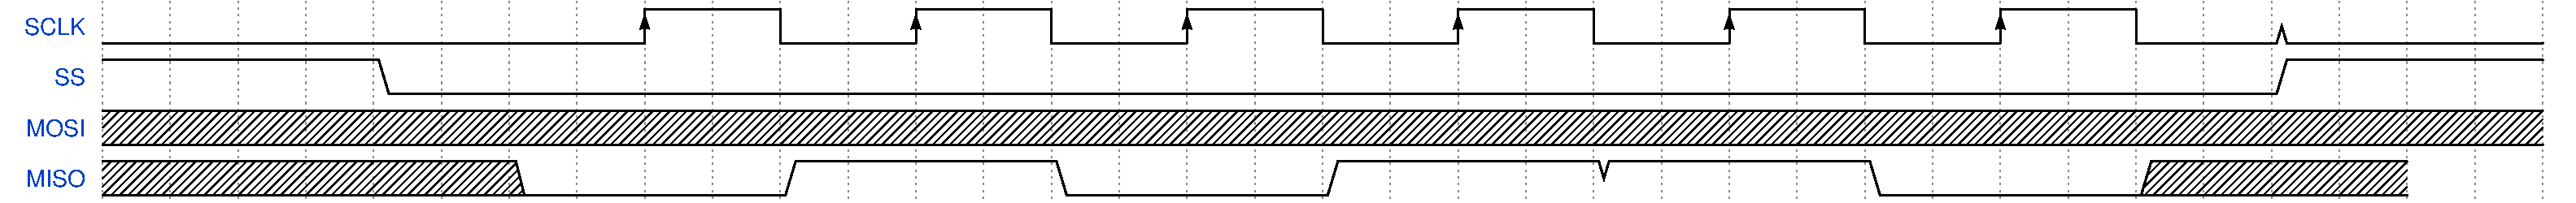
\includegraphics[width=1.00\textwidth]{ondas/SPI_Re.pdf} %0.5
  \caption[Diagrama temporal do envio de dados pelo escravo.]{Diagrama temporal do envio de dados pelo escravo.}
  \label{fig:ondas_SPI_Re}
\end{figure}
 % Thesis_Spi.tex

%%%%%%%%%%%%%%%%%%%%%%%%%%%%%%%%%%%%%%%%%%%%%%%%%%%%%%%%%%%%%%%%%%%%%%%%
%                                                                      %
%     File: Thesis_I2C.tex                        %
%     Tex Master: Thesis.tex                                %
%                                                                      %
%     Author: Carlos A. Rodrigues                         %
%     Last modified : 15 Abril 2013                         %
%                                                                      %
%%%%%%%%%%%%%%%%%%%%%%%%%%%%%%%%%%%%%%%%%%%%%%%%%%%%%%%%%%%%%%%%%%%%%%%

\chapter{I2C}
\label{chapter:i2c}


Explicar o protocolo i2c. como funciona e as linhas que tem. explicar em que acasos é mais usado

por uma imagem os um master e slaves para mostrar como s\~ao as liga\c{c}ões

\section{Mestre I2C}

dizer como estava o master a I2C que n\~ao conseguia enviar ao receber dados.

por um diagrama de blocos de como circula a informa\c{c}\~ao dentro do meu modelo de SPI. fazer uma descri\c{c}\~ao do funcionamento com uma descri\c{c}ao do fluxo de dados.

por a tabela de sinais da interface de i2c (sinais de entrada e saida)

tabela de registos (endere\c{c}os do registos).

explicar os 2 modos de funcionamento de esrita e de leitura que tem 2 modos.

\section{escravo I2C}

processo de constru\c{c}\~ao do escravo 

por um diagrama de blocos de como circula a informa\c{c}\~ao dentro do meu modelo de SPI. fazer uma descri\c{c}\~ao do funcionamento com uma descri\c{c}ao do fluxo de dados.

por a tabela de sinais da interface de i2c (sinais de entrada e saida)

tabela de registos (endere\c{c}os do registos).

explicar os 2 modos de funcionamento de esrita e de leitura que tem 2 modos.
 % Thesis_I2C.tex

%%%%%%%%%%%%%%%%%%%%%%%%%%%%%%%%%%%%%%%%%%%%%%%%%%%%%%%%%%%%%%%%%%%%%%%%
%                                                                      %
%     File: Thesis_Interface_FIFO.tex                        %
%     Tex Master: Thesis.tex                                %
%                                                                      %
%     Author: Carlos A. Rodrigues                         %
%     Last modified : 15 Abril 2013                         %
%                                                                      %
%%%%%%%%%%%%%%%%%%%%%%%%%%%%%%%%%%%%%%%%%%%%%%%%%%%%%%%%%%%%%%%%%%%%%%%

\chapter{Interface FIFO}
\label{chapter:Iter_FIFO}

Nas \ac{ACK} comdições iniciais do projecto seria o systema construido ser capaz de comunicar com dois modelos que seria acrescentados posteriormente ao sistema. Os dois modelos que serão ligados poderam ter frequencia de clock totalmente dististas do sistemas construido. Os modelos que se pretendem ligar são modelos simples que não têm disponível um processador, por essas razão este modelos querem escrever para o sistema que estamos a desenvolver sempre que têm dados, e ler sempre que são imformados que têm dados de leitura.   Por essa razão opetou-se por utilizar um sistema de comunicação simples e que trabalho-se de forma assíncrona. A comunidade Opensource ainda não tinha disponivel qualque cores desenvolvido ou mesmo começado. Por ser uma comunicação de forma simples, assincrona e onde era importante uma elevada de taxa de transferência de dados. Ponderou-se a utilização de duas memorias do tipo FIFO para cada modelo que se pretencia comunicar, onde seria utilizado uma fifo para cada sentido. Como pretendemos uma comunicação rápida entres o sistema e os modelos os dados serão enviados em paralelo permitindo assim uma redução bastante grande do tempo de envio de dados.

Como se pode ver na figura \ref{fig:ligacoesFIFO} este core tem disponível uma interface wishbone para comunicação com o processador do sistema e uma outra interface que utiliza 8 ligações de comunicação, sendo 2 delas de dados utilizando uma para cada sentido. As restantes linhas destinam-se para controlo informando o modelo lá ligado do estado do core. 

\begin{figure}[!htb]
  \centering
  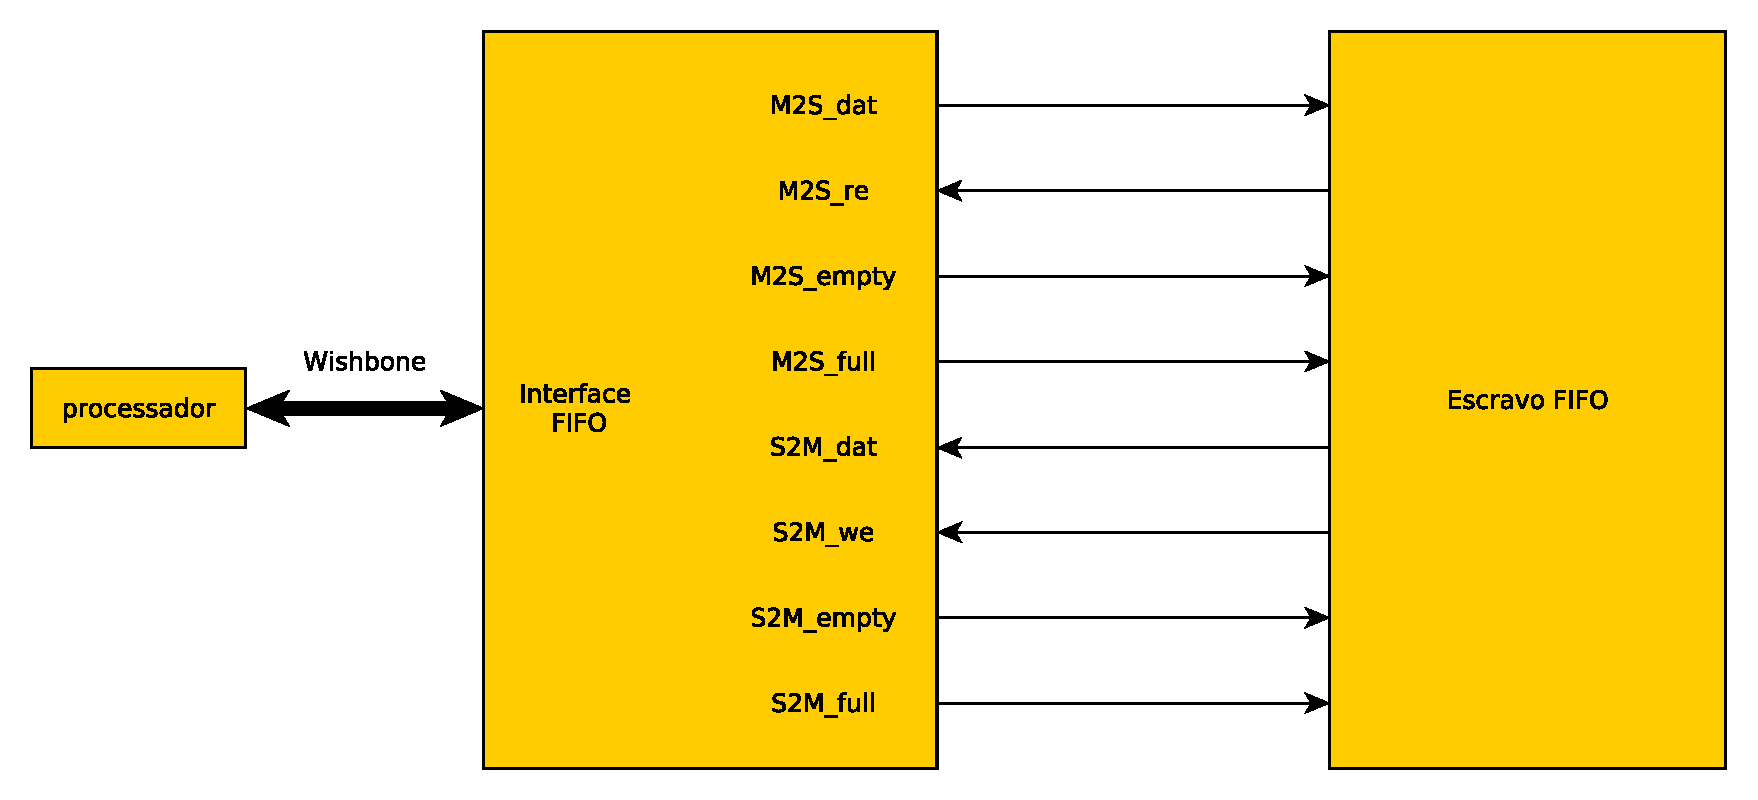
\includegraphics[width=0.75\textwidth]{grafos/FIFO.pdf} %1
  \caption[Protocolo FIFO]{Esquematico do sistema de comunicação FIFO.}
  \label{fig:ligacoesFIFO}
\end{figure}

Como já foi dito antes o core utilizada duas memorias FIFO para a gestão de dados para cada sentido como se pode ver na figura \ref{fig:fluxo_Interface FIFO}. Os dados que são enviado pelo wishbone são guardados na FIFO até o modelo que se encontra do outro lado pedir para o ler. Apenas assim o dados é enviado da memoria FIFO identificada na figura por M2S\_FIFO e envida para o modelo. Quando o modelo pretende enviar dados para o sistemas este envia os dados para a memoria FIFO na figura com o nome de S2M\_FIFO, os dados seram guardado na memorias até o processador pedir mais dados desta interface. O processador antes de enviar ou ler dados da interface deverá ver os estados da memoria correspondente, para o caso de querer enviar dados de verificar se a memoria numerada na figura por M2S\_FIFO não se encontra cheia, para não escrever em cima de dados validos. No caso de pretender ler deverá verificar se a memoria para esse efeito se têm dados, para não ler dados que não fazem sentido. Este procedimento também deverá ser feito pelos modelos que utilizam esta interface, para não haver problemas querencia. 

\begin{figure}[!htb]
  \centering
  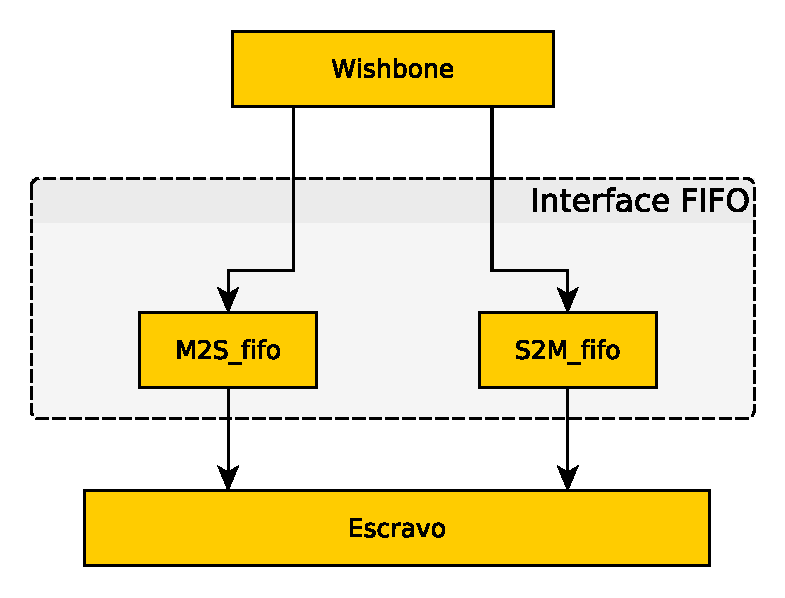
\includegraphics[width=0.50\textwidth]{grafos/diagrama_Interface_FIFO.pdf} % % mudar as setas desta figura.
  \caption[Fluxo de dados do core Interface FIFO]{Fluxo de dados do core Interface FIFO}  
  \label{fig:fluxo_Interface FIFO}
\end{figure}


O core tem dois grandes grupos de linhas de comunicação como se pode ver na tabela \ref{table:sinais_Interface_FIFO}, tem disponível todas as linhas de comunicação wishbone que se encontra ligada ao ao  e a parte de ligações relacionada com o controlo de dados enviados e recebidos pelo outro modelo. O processador pela interface Wishbone tem acesso a informações importantes sobre o cores relacionadas com o estado das duas memorias fifo, permitindo assim este saber quando poder ler dados validos e quando pode enviar dados sem perder dados. O conjunto de ligações da interface FIFO, onde seram ligados os modelos com que se pretendem comunicar.


Como se pode ver na tabela as primeiras quatro ligações são utilizadas para a recepçao e gestão dos dados do sistemas que seram enviados para o outro modelo. As outro quatro ligação são utilizadas para o sentido oposto ou seja para a comunicação e gestão do dados enviados do modelos para para o sistemas que estamos a desenvolver. As linhas identificadas por o sufixo "dat\_i" e "dat\_o" destinasse as ligações para a troca de dados, uma para para entrada de dados e outra para o envio de dados respectivamento, como esta interface é paralela esta duas linhas representam um conjunto de ligações que será do tamanho igual ao tamanho das palavras de dados que pretendemos enviar. Ou seja se pretendemos enviar palavras de 32 bits cada uma destas linhas tem um tamanho de 32 ligações.As linhas identificadas na figura pela sufixo empty e full, empty para vazia e full para cheia, são utilizadas para informar o outro modelo do estado das memorias FIFO's. A linha identificada na figura por M2S\_re é  utilizada pelo outro modelo para informar que está a ler a informação disponível da linha de dados. Por ultimo a linha na figura com o nome M2S\_we informa que os dados que estão na linha de dados de leitura são dados validos para guardar na memoria FIFO.



\begin{table}[h!]
  \begin{center}
    \begin{tabular}{|C{2cm}|c|c|c|}
      \hline
      Interface & Nome & direcção & Descrição \\
      \hline \hline
      \multirow{9}{*}{Wishbone} & clk\_i & input & Clock, Recebido pelo Wishbone. \\
      \cline{2-4}
      & rst\_i & input & Reset, renicia o core quando se encontra no valor logic "1".\\
      \cline{2-4}
	  & cyc\_i & input & \\
      \cline{2-4}
	  & stb\_i & input & \\
      \cline{2-4}
	  & adr\_i & input & Endereço do registo onde se pretende ler ou escrever no core.\\
      \cline{2-4}
	  & we\_i & input & Bit de selecção de escrita.\\
      \cline{2-4}
	  & dat\_i & input & Recepecção de dados por parte do processador.\\
      \cline{2-4}
      & dat\_o & output & Envio de dados para o processador.\\
      \cline{2-4}
      & ack\_o & output & bit que informaça o processador a recepecção do comando pelo core.\\
      \hline \hline
	  \multirow{8}{*}{FIFO} & fifo\_s2m\_dat\_i & input & sinal de entrada de dados do escravo para o mestre. \\
      \cline{2-4}
      & fifo\_s2m\_we & input & sinal de escrita do escravo. \\
      \cline{2-4}
      & fifo\_s2m\_empty & output & sinal da fifo que envia os dados do escravo para mestre se encontra vazia.\\
      \cline{2-4}
      & fifo\_s2m\_full & output & sinal da fifo que envia os dados do escravo para mestre se encontra cheia.\\
      \cline{2-4}
      & fifo\_m2s\_dat\_o & output & sinal de saida de dados do mestre para o escravo\\
      \cline{2-4}
      & fifo\_m2s\_re & input & sinal de leitura do escravo.\\
      \cline{2-4}
      & fifo\_m2s\_empty & output & sinal da fifo que envia os dados do mestre para escravo se encontra vazia.\\
      \cline{2-4}
	  & fifo\_m2s\_full & output & sinal da fifo que envia os dados do mestre para escravo se encontra cheia.\\
      \hline
    \end{tabular}
  \end{center}
  \caption[Tabela de sinais do core Interface FIFO]{Tabela de sinais da interface FIFO}
  \label{table:sinais_Interface_FIFO}
\end{table}

O core necessita de ter do lado do wishbone uma endereço como de pode ver na tabela \ref{table:registos_Interface_FIFO} esta tem apenas 2 endereço. o primeiro com um OFFset de 0X00 sendo o endereço de escrita de de leitura do dados para enviar e enviados pelo modelo. O segundo endereço com o OFFset de 0X02 é um endereço apenas de leitura é onde contem os dados das FIFO.

\begin{table}[h!]
  \begin{center}
    \begin{tabular}{|c|c|c|c|}
      \hline
      Nome & leitura/escrita & Descrição & Offset End. \\
      \hline \hline
      Leitura e escrita de dados& escrita e leitura & Envio ou rececção dos dados& 0X00 \\
      \hline
      Estado fifos & leitura & leitura dos estados das fifos& 0X02 \\
      \hline
    \end{tabular}
  \end{center}
  \caption[Tabela de registo do core Interface FIFO]{Tabela de registos da interface FIFO}
  \label{table:registos_Interface_FIFO}
\end{table}


Sempre e por qualquer das duas interfaces deverá ser feitar uma verificação dos dados na fifo. No caso da leitura da memoria FIFO deverá verificar-se que a memorias não está vazia e no caso da escrita verificar que esta não está cheia. Evitando-se assim no primeiro caso a ler-se dados errados e no segundo caso estar-se a escrever em cima de dados importantes e estes serem perdidos. %Thesis_Interface_FIFO

%%%%%%%%%%%%%%%%%%%%%%%%%%%%%%%%%%%%%%%%%%%%%%%%%%%%%%%%%%%%%%%%%%%%%%%%
%                                                                      %
%     File: Thesis_Bootrom.tex                        %
%     Tex Master: Thesis.tex                                %
%                                                                      %
%     Author: Carlos A. Rodrigues                         %
%     Last modified : 15 Abril 2013                         %
%                                                                      %
%%%%%%%%%%%%%%%%%%%%%%%%%%%%%%%%%%%%%%%%%%%%%%%%%%%%%%%%%%%%%%%%%%%%%%%

\chapter{Bootrom}
\label{chapter:Bootrom}

Quando um sistema arranca ou seja é dada energia ao sistema, este faz resite a todos os cores até mesmo ao processador. Depois do resite o processador vai ao endereço que é atribuido pela pessoas que desenvolver o sistema e carrega e carrega essa informação para o registo para começar a desenvolver o processo que está descrito a partir dessa posição de memoria. A partir daqui existe duas grande hipoteses, a primeira hipotese é o programa estar estar carregado na memoria de instruções partida. Tendo apenas o endereço de restart ser o endereço da memoria de instruções e ser o endereço onde começara o programa, este hipotese tem a vantagem de ser mais simples e de ter um restart mais rápido, começando o programa a correr assim que o sistema recebe energia, mas tem a desvantagem de o programa não poder ser alterado facilmente. a segunda Hipoetese é o endereço definido no restart ser um endereço para uma bootrom que tem disponível uma pequeno programa que copia o programa de uma memoria externa para a memoria de instruções, no fim de acabar esse processor coloca o o ponteiro do estrições para o endereço onde começa o programa que copiou de forma a executar o programa. esta segunda hipotese demora mais tempo o programa a iniciar, mas permite que o programa que se está a correr seja alteração de uma forma simples. Como por exemplo substituir um cartão de memoria e ligar e desligar a energia eléctrica do sistema. Uma bootrom é como o nome indica uma memoria Rom, apenas permite leitura, na maorias dos casos onde contem um pequeno programa normalmente escrito em assemble para ser mais pequeno e eficiente. Esse programa apenas copia os dados de uma determinado local para a memoria de instruções, podendo também fazer algumas pequenas verificações.

No desenvolvimento do projecto optou-se por utilizar uma bootrom por permitir uma alteração simples do programa que se estava a correr no sistema. A a comunidade openRisc tinha disponivel bastante simples que copiava os dados de HHHHH posições de memorias comeraçando de uma posição de endereços de periférico para outro endeço on estava localizado a sura memoria de enderços.
Mas era pretendido mais do que isso, para alem de copias essas posições de memoria pretendia-se que efectua-se verificações na correcta leitura da memoria onde o programa principal estava guardado e verificação de uma escrita correcta para a memoria de instruções. Para isso desenvolvemos uma bootroom que estão descrita no fluxograma \ref{fig:Fluxo_Bootrom} de uma forma sucinta.

escrever que isto é compilado e é possivel desactivar as cada mensagem de erro.

\begin{figure}[!htb]
  \centering
  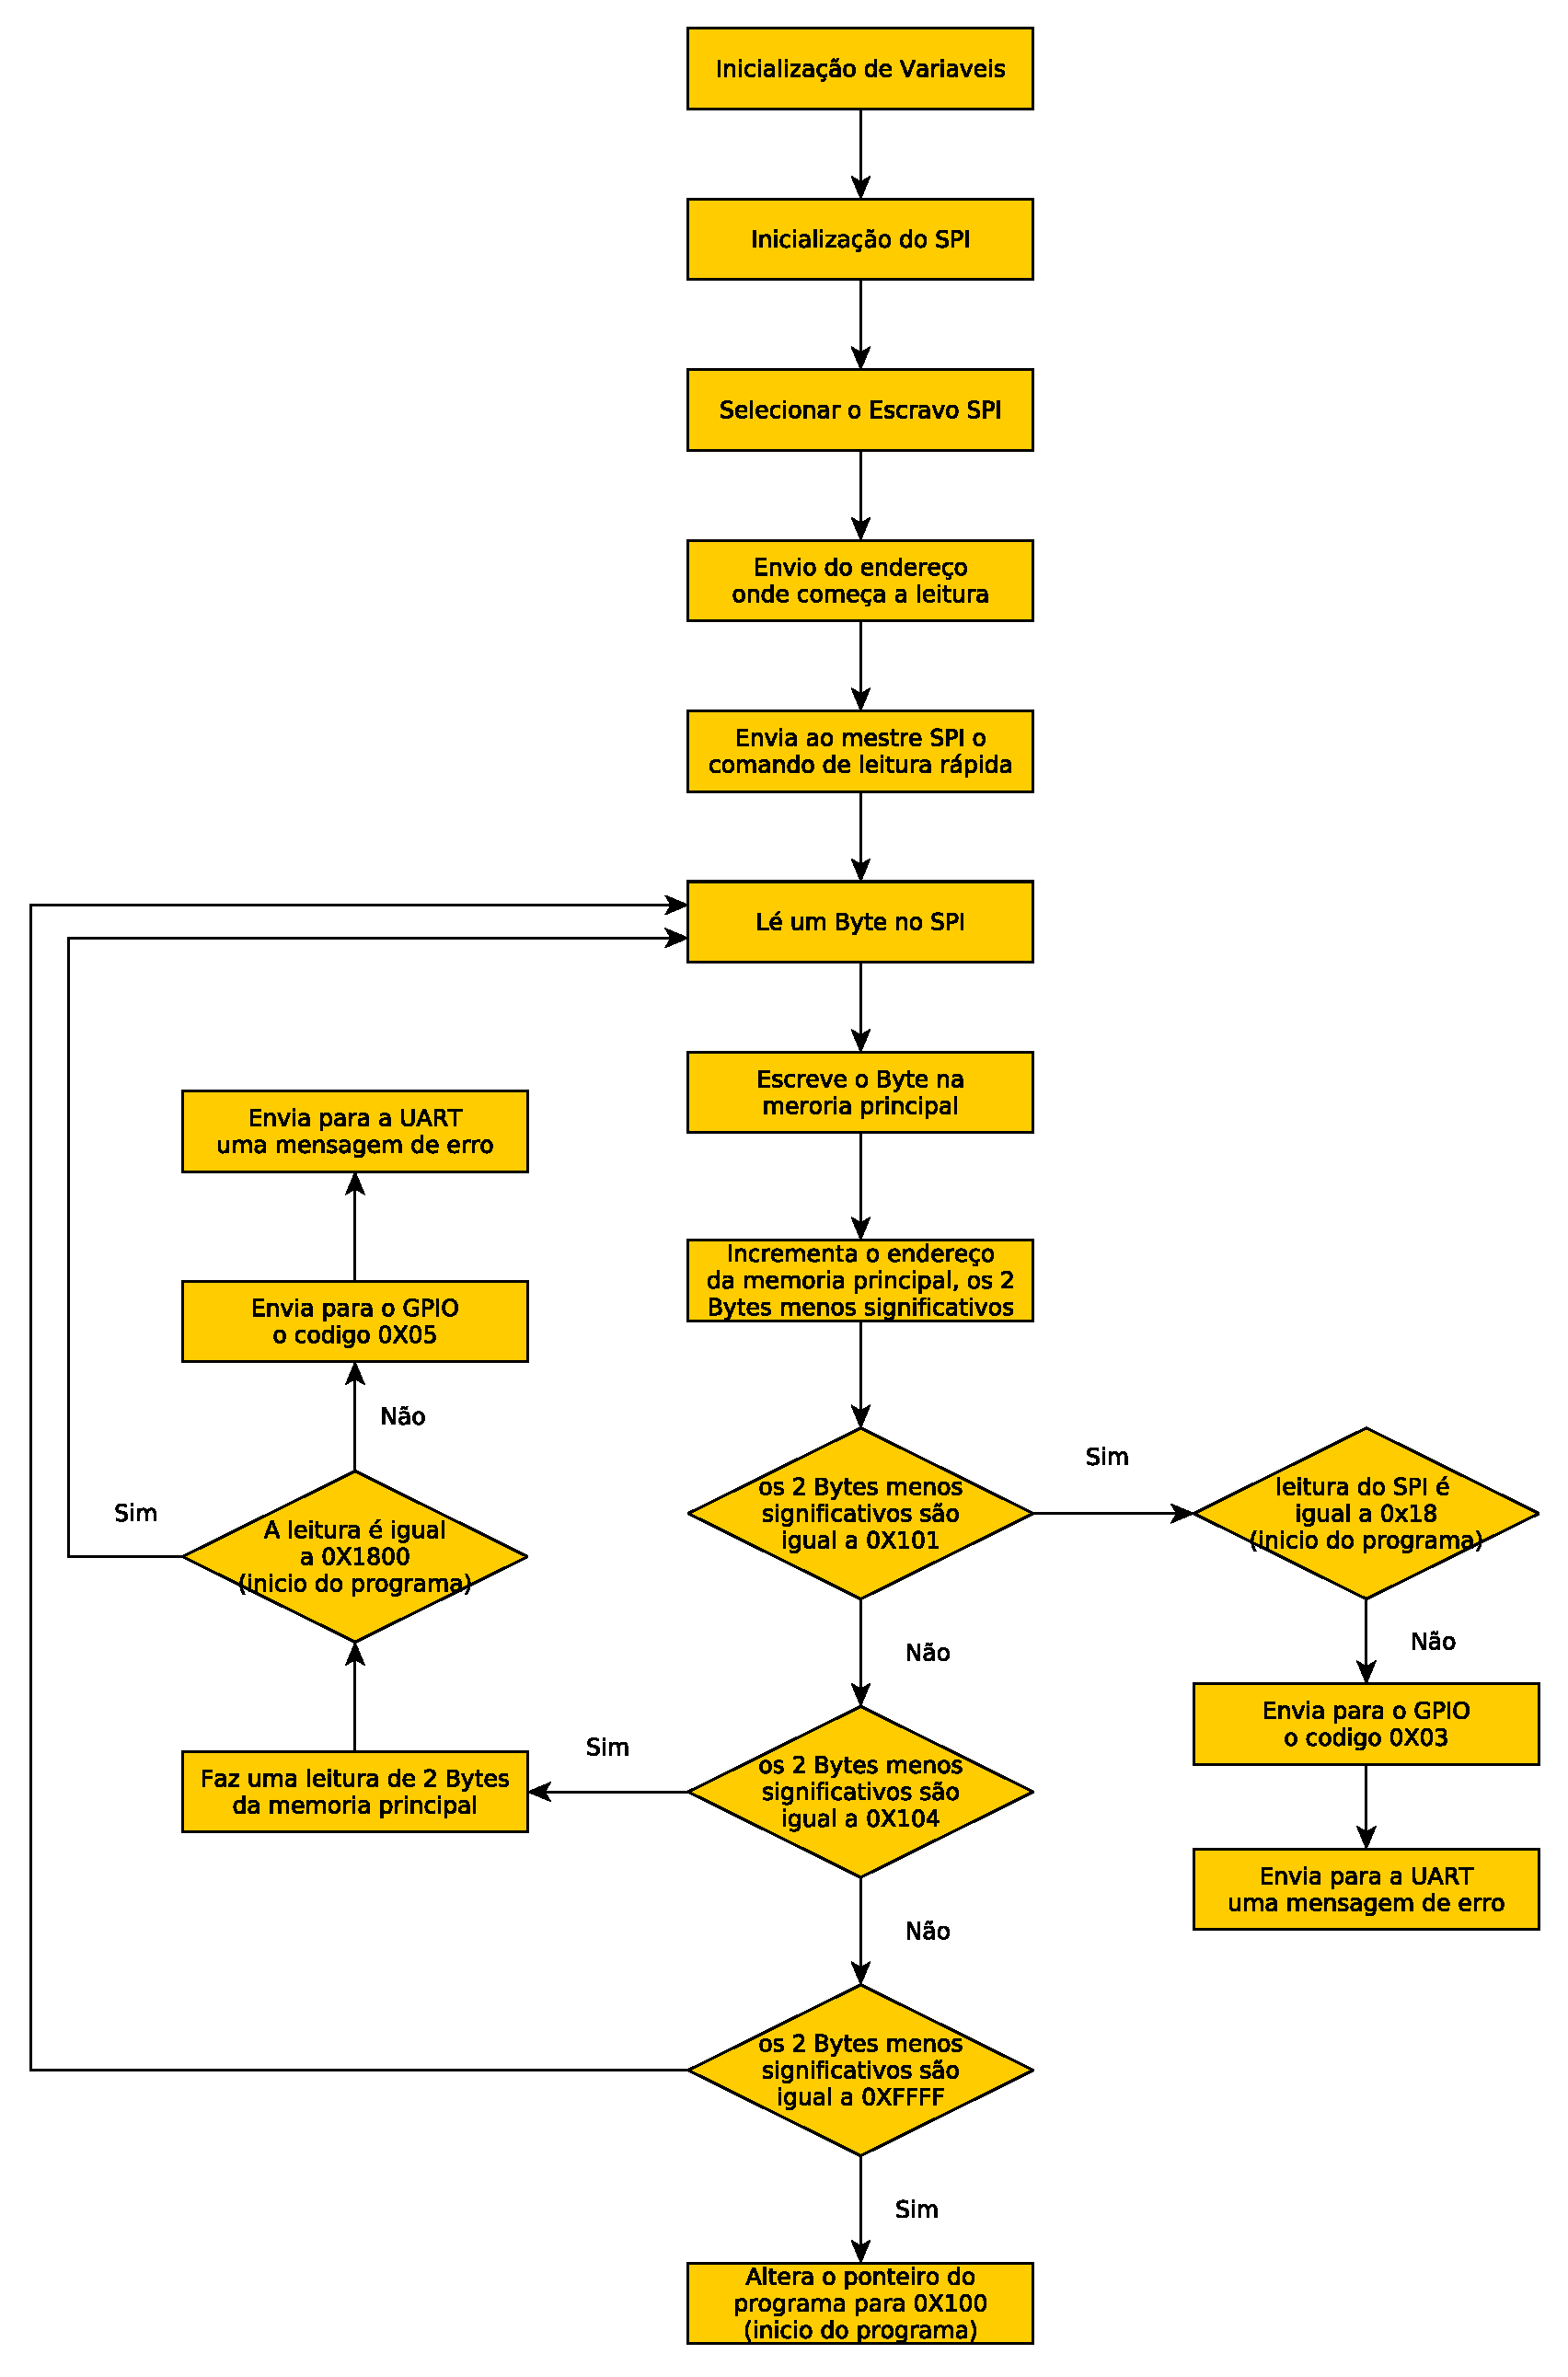
\includegraphics[width=0.75\textwidth]{grafos/Bootrom.pdf} %1  falta uma seta no fluxograma num exagno
  \caption[Fluxograma da Bootrom]{Fluxograma da Bootrom.}
  \label{fig:Fluxo_Bootrom}
\end{figure}

Como se pode ver pelo fluxograma a bootrom começa por iniciar os registo do processador, depois configura o core SPI. Inicializando o core mestre de SPI, informa o endereço que deve começar a ler da memroia e informar o tipo de leitura que pretende fazer neste caso a rápida. Começa a fazer uma leitura consegutiva de 0XFFFF(65535 na base decimal) posições de memoria, com palavras de tamanho de Byte. Quando acaba o envio de todas posições de memoria efetua uma salto do porteiro de instruções para a memoria de instruções para o endereço onde começa o programa, começando a correr o programa que estava na memoria externa. No ciclo que estão a efectuar a copia de uma memoria para outra, é efectuado dois testes para verificar que a correcta leitura e escrita das memorias. Quando é detectado um erro, este o core envia mensagens de erro tanto pela UART enviado uma mensagem de erro, e pela interface disponiblizada de GPIO envido um código de mensagem 0X03 se for problema de leitura da memoria externa e 0X05 se for problema de escrita na memoria interna.

\section{Testes de verifica\c{c}\~ao}
Os testes de verificação de leitura e escrita para verificar se foi correctamento um carregamento do programa na memomeria principal. Para isso foi desenvolvido um teste para cada caso de leitura dos dados da memoria externa que é lida por SPI e outro teste que verifica se foi escrito corretamente na memoria de instruções. 

\subsection{teste de leitura SPI}

O primeiro teste a ser efetuado é o teste de leitura das insctruções do programa da memoria externa por SPI. Todos os programas compilados têm a mesma instrução inicial 0X?????, na mesma posição de memoria 0X????. Neste teste ele everifica se os dados da posição de memoria 0X???? corresponden aos dados da instrução inicial. Como a memoria extrena tem apenas dois Bytes por cada posição o teste verifica os dois primeiro bytes da primeira instrução. Se os dados forem os esperados os ele continua a copias as instruções para a memoria de instruçoes se não, para de efectuar a copia dos instruções e enviar mensagens de erro tanto por GPIO como por UART. Quando detectado o processador envia um codigo de erro 0X?? para o GPIO e em seguida enviará a seguinte mensagem " mensagem XXX" pela UART. Caso tenha uma "leitor" de UART ligado ao sistema receberá a mensagem no meu leitor.

\subsection{teste de escrita na memoria principal }

O processo de teste é efectuado quando o processo de escrita para a memoria principal escreve os primeiros 4 Bytes de insctuções, correspondenedo ao endereço 0XWWWW da memoria principal. Quando a condição anterior é verdadeira a escrita de instruções é interrumpida momentaniamente, e é efectuado uma leitura de 4bytes do endereço  0XWWWW, que foi acabado de ser escrito. para verificar se as instruções estão a ser escritas correctamente a palavra lida na memoria principal tem de ser o valor 0XPPPPP, caso contrario existe algum erro no processo de escrita. Caso o teste seja positivo o processo continua normente a copiar as instruções do programa para a memoria principal, se não é dispuldado a seguinte mensagem de erro para a UART " mensagem de erro" do sistema e é colocado o seguinte codigo TT no GPIO.

explicar como é feito o teste de escrita na memoria principal 

como mostra o erro tanto com o GPIO como na uart. %Thesis_Bootrom

%%%%%%%%%%%%%%%%%%%%%%%%%%%%%%%%%%%%%%%%%%%%%%%%%%%%%%%%%%%%%%%%%%%%%%%%
%                                                                      %
%     File: Thesis_Bootrom.tex                        %
%     Tex Master: Thesis.tex                                %
%                                                                      %
%     Author: Carlos A. Rodrigues                         %
%     Last modified : 15 Abril 2013                         %
%                                                                      %
%%%%%%%%%%%%%%%%%%%%%%%%%%%%%%%%%%%%%%%%%%%%%%%%%%%%%%%%%%%%%%%%%%%%%%%

\chapter{Testes de funcionamento}
\label{chapter:teste}

explicar para que quero os testes.

como foi implementado no Orpsoc. 

adicionar uma imagem explicativa como foi implementado.

falar sobre as flags do teste

como posso ver os resultados dos teste

\section{adicionar novos testes}

fazer novos testes.

\section{Testes desenvolvidos}

para mostrar que o sistema funciona corremante foi desenvolvido estes testes 

\subsection{SPI}

explicar como é testado

\subsubsection{simulador verilator}

\subsubsection{Board VGA}

\subsection{I2C}

explicar como é testado

\subsubsection{simulador verilator}

\subsubsection{Board VGA}

\subsection{Interface FIFO}

explicar como é testado

\subsubsection{simulador verilator}

\subsubsection{Board VGA}

\subsection{Bootrom}

explicar como é testado

\subsubsection{simulador verilator}

\subsubsection{Board VGA}
 %Thesis_Teste

%%%%%%%%%%%%%%%%%%%%%%%%%%%%%%%%%%%%%%%%%%%%%%%%%%%%%%%%%%%%%%%%%%%%%%%%
%                                                                      %
%     File: Thesis_Results.tex                                         %
%     Tex Master: Thesis.tex                                           %
%                                                                      %
%     Author: Gonçalo Santos                                           %
%     Last modified : 20 Oct 2018                                      %
%                                                                      %
%%%%%%%%%%%%%%%%%%%%%%%%%%%%%%%%%%%%%%%%%%%%%%%%%%%%%%%%%%%%%%%%%%%%%%%%

\chapter{Results}
\label{chapter:results}

The aim of this work is to produce a workable {\bf C} language
compiler for the {\it Versat} architecture using the {\it picoVersat}
instruction set.
The success can be measured by the number of {\bf C} language
constructs that are working properly.
Consequently, testing is of primordial importance, as are the range
of tests used to exercise the compiler.

\section{Functionality}

The compiler, as far the tests were comprehensive,
supports all {\bf C} language integer constructs.
Limitations are listed below.

Since the processor instruction set is reduced, as are the
number of {\bf lcc} terminals to be implemented by the compiler,
the testing of each operation, on its own, is strait
forward.
Testing sequences of such operations may prove more
difficult to test, since different {\bf C} programs
can produce different selection matches.

\section{Testing}

In the test of a compiler, where a small change can affect the
generation of multiple instructions, a good set of
regressive tests is very important.
In order to automate the process, a {\tt test/} directory
was setup.
This directory includes a set of {\bf .c} test files and
the expected output {\bf .out}.

The {\tt Makefile} compiles, executes and compares the new
result with the previously stored result.
All differences in output are printed and can then be analyzed.

Since the output from {\bf iverilog} includes the number
of clocks spent, it is easy to compare whether the changes in the
compiler result in improvements, or in performance degradation.

Some tests are very simple and its output can be easily predicted.
To make testing even simpler, the return value of the {\tt main}
routine is printed, unless the {\sc NORET} environment variables
is defined. Upon return from the {\tt main} routine, the lowest
nibble is printed as an {\sc ASCII} starting at $0$.
This means that values between $10$ and $15$ are printed as
the {\sc ASCII} character at the respective offset, namely the
sequence: \verb|:|, \verb|;|, \verb|<|, \verb|=|, \verb|>|, \verb|?|.

More complex tests can be compiled with {\bf gcc} and executed
to access the expected output.
This, however, can not be performed if the examples include
{\tt asm} calls, since the code can only be executed by the
{\it Versat}, or by the {\bf iverilog} simulator, and not by the
native testbench processor.
%vdb.c

A set of $86$ regression tests is currently being used, ranging
from specific operator testing to complex recursive and iterative
examples. % And the number of tests keeps growing ...

\section{Limitations}\label{limitations}

The {\bf C} language imposes that {\tt sizeof(char)==1}
as does the {\bf lcc} compiler (see~\cite[p.79]{hanson95}).
This works fine as far as {\tt sizeof(char)} can be 32-bits.
However, additionally, the {\bf lcc} assumes through out
the code that $8$ is the number of {\em bit-per-byte}.
If it was a variable, one could set it to $32$.
As it is hardcoded, all address literals
will be truncated to 8-bits ({\tt 8}${}^{\wedge}${\tt ty->size}).
\begin{verbatim}
int *addr = (int*)0x123456;
\end{verbatim}
This can be avoided by setting an integer to the
required value and then assigning it to a pointer.
This works since integer literals are 32-bit wide
and the conversion to pointer, controlled by the
{\it back-end}, does not truncate the value.
\begin{verbatim}
int *addr, value = 0x123456;
addr = (int*)value;
\end{verbatim}
Nevertheless, defining literal pointer is never
a good predictive in virtual memory machines.
In {\it Versat} it is useful to map variables
to specific addresses.

Due to the same reason, a warning message is issued
({\tt shifting an `int' by 12 bits is undefined})
but the code is correctly generated.

% #define LONG_MIN -2147483648
% warning: unsigned operand of unary -
% but 0x80000000 or bellow is OK!
% #  define LONG_MAX	2147483647
% #  define LONG_MIN	(-LONG_MAX - 1L)

In the initial version of {\it picoVersat}, all global
data must be added by {\tt MEM\_BASE=512}.
Since this is performed when addresses are fetched,
static assignments store the unadded value.
Therefore, all accesses must be added by $512$.
Must add {\tt 512} to global pointers in {\tt picoversat-0.0}
\begin{verbatim}
int mem[10], *base = mem;
int main() { base[6+512] = 9; return return mem[6]; }
\end{verbatim}
This can be avoided if assignment is performed during
execution (not at compile time), even if the variable
is global.
\begin{verbatim}
int mem[10];
int main() { int *base = mem; base[6] = 9; return return mem[6]; }
\end{verbatim}

Signed multiplication, division and modulus ({\tt \_mul},
{\tt \_div} and {\tt \_mod}) do not generate carry since
the flags register of {\it picoVersat} is read-only.

The {\bf C} programming languages relies on separate
compilation, where several files are independently
compiled and then linked together.
However, there is no linker in the {\it Versat} system
and the assembler {\bf va} does not support multiple
files.
The solution is to perform linking with {\bf cpp} %%%
include directives.
While in normal {\bf C} the {\tt .c} should be
included, rather compiled, the inclusion of {\bf .h}
as well as {\bf .c} accomplishes the desired result.
Since there is no linking, only multiple inclusion
of files must be avoided.

The {\it Versat} architecture is meant to be used offline
and no form of argument passing to the {\tt main} routine
is available.
Consequently, the stack is initialized at the top.
Therefor, even if the program declares arguments to
the {\tt main} routine ({\tt argc, argv, envp}) they should
never be accessed.
Also, since the system has no memory management unit,
all illegal accesses are silently ignored by the system.
Highly recursive routines that exhaust the stack will have
unpredictable behaviors, since they will begin to overwrite
the top of the code.
Even if it is not the compilers responsibility, it something
that the programmer should be aware, especially when
transitioning from a virtual managed memory system.

Finally, the compiler does not support floating point
data types, since every operation must be supported
by library routines.
This is the case for many android devices, namely
smartphones.
However, the {\it Versat} purpose is to perform
integer arithmetic operations fast and is not aimed at
scientific programming.
The error message {\tt compiler error in \_label--Bad terminal}
is issued by the compiler when it cannot handle a given operation,
namely floating point operations.

\section{Register assignment}

Register assignment in compiler design considers two types of registers:
global registers that hold variable values and scratch registers that hold
temporary values.
The {\bf lcc} compiler defines these registers by setting a mask for each
type of register.
It is up to each {\it back-end} to define the mask values according to processor
capabilities.
For instance, the {\bf sparc} processor defines $4$ sets of $8$ registers:
global, temporary, input and output; where the later two sets replace
the stack for argument passing.
In {\bf i386} all $7$ registers are temporary, while {\bf mips} uses half
for each purpose ($16+16$).

Since the {\it picoVersat} has no specific register assignment, a study
was carried out in order to assess the best balance between global and
scratch registers.
Registers {\tt R0} and {\tt R13} to {\tt R15} are used to communicate with {\it Versat}
and are invisible to the compiler.
The stack is controlled by a {\it stack pointer} ({\tt R12}) and a {\it frame pointer}
({\tt R11}).
The remaining registers ({\tt R1} to {\tt R10}) compose a mask {\tt 7FE}, where
the lowest bit ({\tt R0}) is omitted for register assignment, and the highest
used bit {\tt 400} is {\tt R10}.
The register {\tt R1} is used to return function values and all arguments are
passed on the stack.
At least two registers must be used as scratch for binary operations
temporaries.
The compiler allows the definition of a {\tt tmask} for temporaries and a
{\tt vmask} for variables.

Initially, in run $1$, the experiment uses all registers for temporaries.
Each run adds a variable register at the expense of a temporary, until only
two temporaries remain (run $9$).
Three examples where used: {\tt assign}, {\tt repeating locals} and
{\tt bubble sort}.
The first two represent opposite extremes of register usage, while the last is
a more balanced and realistic example.

The first example uses the {\bf C} language right associative {\it assign} operator
where each new assignment to the variable {\tt a} requires a new temporary register.
%(see Figure~\ref{fig:assign}).

%\begin{figure}
\begin{verbatim}
int f() { return 1; }
int main()
{
  int a;

  a = f() + (a =
      f() + (a =
      f() + (a =
      f() + (a =
      f() + (a =
      f() + (a =
      f() + (a =
      f() + (a =
      f() + (a =
      f() + (a =
      f() + (a =
      f() + (a =
      f() + (a = 1
                  )))))))))))));
  return a;
}
\end{verbatim}
%\caption{}
%\end{figure}

The register usage shows that each assign uses a register $4$ times at
the expense of the return register {\tt R1}.
The best solution, represented by the lowest clock count,
is to use only two temporaries, since more variables imply more stack ({\tt R12}),
saves and restores between each call to the function {\bf f}.

%\begin{table}
\begin{center}
{\small
\begin{tabular}{r|r|r|r|r|r|r|r|r|r|r|r|r|r|r|r|r}
run&vars&vmask&tmask&R1&R2&R3&R4&R5&R6&R7&R8&R9&R10&R11&R12&clks\\\hline
1&0&000&7FE&21&4&4&4&4&4&4&4&6&44&27&82&677\\
2&1&400&3FE&23&4&4&4&4&4&4&6&42&17&14&82&638\\
3&2&600&1FE&25&4&4&4&4&4&6&42&0&17&16&77&633\\
4&3&700&0FE&27&4&4&4&4&6&42&0&0&17&18&72&628\\
5&4&780&07E&29&4&4&4&6&42&0&0&0&17&20&67&623\\
6&5&7C0&03E&31&4&4&6&42&0&0&0&0&17&22&62&618\\
7&6&7E0&01E&33&4&6&42&0&0&0&0&0&17&24&57&613\\
8&7&7F0&00E&35&6&42&0&0&0&0&0&0&17&26&52&608\\
9&8&7F8&006&39&42&0&0&0&0&0&0&0&17&28&47&603\\
\end{tabular}
}
\end{center}
%\caption{}
%\end{table}
\vspace*{5mm}

The second example uses lots of repeating local variables so that each one is assigned
a register, for its uses from the first to last line, if one is available.
%(see Figure~\ref{fig:locals}).

%\begin{figure}
\begin{verbatim}
int func(int a, int b, int c, int d, int e, int f, int g, int h, int i, int j, int k) {
    a = a + b - c - d - e + f - g + h + i + j + k;
    b = a - b + c + d - e - f + g - h + i - j - k;
    c = a + b - c - d + e + f + g - h + i + j - k;
    d = a - b - c + d - e + f - g + h - i - j - k;
    e = a + b + c - d - e - f - g + h - i + j - k;
    f = a - b - c + d - e + f + g - h - i - j + k;
    g = a + b - c - d + e + f + g - h + i + j - k;
    h = a - b + c + d - e - f - g + h + i - j - k;
    i = a + b - c - d - e + f + g + h + i + j - k;
    j = a - b - c + d - e + f + g - h - i - j - k;
    k = a + b + c - d + e - f - g - h - i + j + k;
    return a + b + c + d + e + f - g + h - i + j - k;
}

int main() {
    return func(10, 9, 8, 7, 6, 5, 4, 3, 2, 1, 0);
}
\end{verbatim}
%\caption{}
%\end{figure}

As expected, the best solution is to use highest of temporaries in order
to reduce frame pointer ({\tt R11}) accesses to stack saved values.

%\begin{table}
\begin{center}
{\small
\begin{tabular}{r|r|r|r|r|r|r|r|r|r|r|r|r|r|r|r|r}
run&vars&vmask&tmask&R1&R2&R3&R4&R5&R6&R7&R8&R9&R10&R11&R12&clks\\\hline
1&0&000&7FE&45&27&12&13&48&46&40&45&54&62&68&56&956\\
2&1&400&3FE&53&31&13&54&46&40&47&54&62&0&78&51&1001\\
3&2&600&1FE&61&35&52&46&48&49&56&62&0&0&89&46&1051\\
4&3&700&0FE&89&39&59&63&51&56&62&0&0&0&101&41&1106\\
5&4&780&07E&109&43&75&49&74&79&0&0&0&0&113&36&1161\\
6&5&7C0&03E&146&45&84&58&105&0&0&0&0&0&124&31&1211\\
7&6&7E0&01E&156&88&112&94&0&0&0&0&0&0&138&26&1278\\
8&7&7F0&00E&171&117&176&0&0&0&0&0&0&0&154&21&1356\\
9&8&7F8&006&231&249&0&0&0&0&0&0&0&0&172&16&1447\\
\end{tabular}
}
\end{center}
%\caption{}
%\end{table}
\vspace*{5mm}

The last example, the {\it bubble sort}, uses a mixture temporaries and variable
reuses. %(see Figure~\ref{fig:bubble}).

%\begin{figure}
\begin{verbatim}
#include "printi.h"

int bubble(int list[], int n) {
    int c, d, t, swap, cnt = 0;

    for (c = 0; c < n - 1; c++) {
        for (swap = 0, d = n - 1; d > c; d--)
            if (list[d - 1] > list[d]) {    /* Swapping */
                swap++;
                t = list[d];
                list[d] = list[d - 1];
                list[d - 1] = t;
            }
        if (!swap)
            break;
        cnt++;
    }
    return cnt;
}

int v[] = { 7, 4, 9, 6, 2, 1, 3, 5, 8, 0 };

int main() {
    int i, size = sizeof(v) / sizeof(v[0]), cnt = bubble(v, size);
    for (i = 0; i < size; i++) {
        putchar(v[i] + '0');
        putchar(' ');
    }
    printi(cnt, 10);
    putchar('\n');
    return 0;
}
\end{verbatim}
%\caption{}
%\end{figure}

This example exploits the tradeoff between global and temporary register
usage.
In the first runs the compiler is unable to use all temporaries.
In the last runs some variable registers are left unassigned and the number
of required execution clocks rises again.

%\begin{table}
\begin{center}
{\small
\begin{tabular}{r|r|r|r|r|r|r|r|r|r|r|r|r|r|r|r|r}
run&vars&vmask&tmask&R1&R2&R3&R4&R5&R6&R7&R8&R9&R10&R11&R12&clks\\\hline
1&0&000&7FE&2&0&0&0&0&4&5&15&30&45&31&36&9855\\
2&1&400&3FE&2&0&0&0&0&4&7&29&41&11&24&36&8193\\
3&2&600&1FE&2&0&0&0&4&5&27&37&7&11&19&41&7714\\
4&3&700&0FE&2&0&0&0&5&25&37&4&7&11&17&41&7399\\
5&4&780&07E&2&0&0&5&19&37&6&4&7&11&13&46&7022\\
6&5&7C0&03E&2&0&5&19&33&6&6&4&7&11&9&49&6949\\
7&6&7E0&01E&2&5&19&33&0&6&6&4&7&11&9&49&6949\\
8&7&7F0&00E&5&19&33&0&0&6&6&4&7&11&9&44&6921\\
9&8&7F8&006&21&28&0&0&0&6&6&4&7&11&13&41&7492\\
\end{tabular}
}
\end{center}
%\caption{}
%\end{table}
\vspace*{5mm}

Based on experience with the examples above, a balanced approach should work best
in most cases.
Therefor, the first five registers, {\tt R1} to {\tt R5}, are used as temporaries
({\tt tmask=0x003E}) and the remaining five, {\tt R6} to {\tt R10}, are used as
variables ({\tt vmask=0x07C0}).

\section{Efficiency considerations}

Calls are very expensive operations for any processor.
{\it Intel Inc.} has made a significant effort over the year to address this
problem.
In the last years, its high end processors provide faster {\it calls} than
{\it jumps} at the expense of higher transistor count. %ref!
In a processor like {\it picoVersat}, the problem is magnified since
no stack specific registers or opcodes are available.

A function call in the {\bf C} programming language requires:
\begin{enumerate} \itemsep0em 
\item {\bf argument passing} by pushing values to the stack;
\item {\bf calling} the desired routine;
\item {\bf saving used registers} before the routine destroys its values;
\item {\bf frame pointer} saving to access arguments and locals;
\item {\bf allocate space} for local variables;
\item actually performing the routine operations;
\item {\bf restoring frame pointer} of the previous routine;
\item {\bf restoring used registers} previous values;
\item {\bf returning} to the calling routine;
\item {\bf removing arguments} from stack.
\end{enumerate}
The present compiler detects when a routine accesses no arguments or locals
and does not emit frame pointer code. So, if a routine only uses global
variables, the call becomes a bit more efficient.
Some of the tests used become upto 5\% faster by removing the frame
pointer in routines where it not needed.

As any routine can be called many times, even recursively, the compiler
must save, at the beginning, and restore, at the end,
all the registers the routine uses.
This means that, at the start of the program, the {\tt main} routine will spill
all registers it will use, although they have no defined value.
Such procedure is required since the routine may be recursively called.
However, in most cases, the {\tt main} routine is only invoked once, at
the start of the program.
The {\sc NOSAV} environment variable can be set if the {\tt main}
routine is not used recursively and no registers will saved by the compiler.
This special hack can be dangerous to use, but it makes {\tt main} based
programs more efficient.

The {\it picoVersat} controls {\it Versat} by setting specific values to
predefined memory positions.
The use of a routine to perform such a task is a very
expensive way to change memory positions, either through {\tt asm}
directives or standard {\bf C} code, as the tests {\tt set.c} and
{\tt setvar.c} show, respectively.
Memory values can be efficiently changed by assigning to a pointer
{\tt *addr=val} (see Limitations, above).

During this work, the {\it picoVersat} evolved. The use of a single
memory, for program code and data, removed the need for a {\tt addi MEM\_BASE}
instruction for each variable load and store, resulting in a 5\% improvement
over all the regression test in use, at the time. % 17022/16213 pico-0

Finally, the compiler some times generates a register read after the
same register was written by another instruction selection.
At least, the read can be suppressed, but {\bf lcc} provides no
peephole optimizer for final code cleanup.

\section{Compiler instalation}

The compiler itself, {\bf lcc}, can be invoqued directly with the
{\tt -target=versat} option, as long as the input file has already
been preprocessed ({\bf cpp}).
The compiler output is a {\it picoVersat} assembly, that can then
fed to the {\it versat} assembler ({\bf va}).

However, the complete compilation process, from {\bf C} language
source file to {\bf iverilog} simulation executable, can be
integrated as in a standard high-level compiler.

Section~\ref{app:integ} describes the requirements for such an integration.
The compiler {\tt Makefile}s, in the main and {\tt versat/} directories,
can be used to provide the instalation of all required files
for a complete development environment.
By default, without any changes to the {\tt Makefile}s, the
compiler development environment is placed under the
{\tt /usr/local/versat} directory.

The default directories for the compiler installation
({\tt make install}) are predefined as
{\tt /usr/local/versat/lcc} for the compiler files
({\tt lcc}, {\tt cpp}, {\tt rcc}, {\tt va}, and
{\tt xdict.json}), and can be redefined at compile
time or using the {\sc LCCDIR} environment variable
at runtime. The {\it picoVersat} {\tt rtl/} files
({\tt include/}, {\tt src/}, and {\tt testbench/})
should be copied to {\tt /usr/local/versat/pico}
(defined at compile time).
Also the {\bf iverilog} compiler is defined at
compile time as residing in {\tt /usr/local/bin/}.

The structure of the installed files,
in the current version is:
\begin{Verbatim}[baselinestretch=1.0]
/usr/local/versat/lcc/lcc
/usr/local/versat/lcc/cpp
/usr/local/versat/lcc/rcc
/usr/local/versat/lcc/va
/usr/local/versat/lcc/xdict.json
/usr/local/versat/lcc/include/strlen.h
/usr/local/versat/lcc/include/umod.h
/usr/local/versat/lcc/include/errno.h
/usr/local/versat/lcc/include/malloc.h
/usr/local/versat/lcc/include/umul.h
/usr/local/versat/lcc/include/itoa.h
/usr/local/versat/lcc/include/Makefile
/usr/local/versat/lcc/include/stdarg.h
/usr/local/versat/lcc/include/mem_ends.h
/usr/local/versat/lcc/include/xdict.h
/usr/local/versat/lcc/include/atoi.h
/usr/local/versat/lcc/include/puts.h
/usr/local/versat/lcc/include/dma.h
/usr/local/versat/lcc/include/versat.h
/usr/local/versat/lcc/include/ends.h
/usr/local/versat/lcc/include/mul.h
/usr/local/versat/lcc/include/xdictinc
/usr/local/versat/lcc/include/div.h
/usr/local/versat/lcc/include/ends.cbc
/usr/local/versat/lcc/include/udiv.h
/usr/local/versat/lcc/include/printf.h
/usr/local/versat/lcc/include/mod.h
/usr/local/versat/lcc/include/alloca.h
/usr/local/versat/lcc/include/printi.h
/usr/local/versat/lcc/include/gnuc.h
/usr/local/versat/lcc/include/putchar.h
/usr/local/versat/lcc/include/assign.h
/usr/local/versat/pico/testbench/sim_xtop.cpp
/usr/local/versat/pico/testbench/xtop_tb.v
/usr/local/versat/pico/include/xdefs.vh
/usr/local/versat/pico/src/xaddr_decoder.v
/usr/local/versat/pico/src/xctrl.v
/usr/local/versat/pico/src/xram.v
/usr/local/versat/pico/src/xregf.v
/usr/local/versat/pico/src/xcprint.v
/usr/local/versat/pico/src/xtop.v
\end{Verbatim}

After adding the {\tt /usr/local/versat/lcc} directory to
the {\sc PATH} environment variable, an executable example
can be produced with the command:\\
{\tt lcc example.c -o example}

The example can then be run with:\\
{\tt ./example}

Please note that the {\it versat} memory dump {\tt .hex}
file is stored in the {\tt /tmp} directory.

\cleardoublepage
 % file "Thesis_Results.tex"

%%%%%%%%%%%%%%%%%%%%%%%%%%%%%%%%%%%%%%%%%%%%%%%%%%%%%%%%%%%%%%%%%%%%%%%%
%                                                                      %
%     File: Thesis_Conclusions.tex                                     %
%     Tex Master: Thesis.tex                                           %
%                                                                      %
%     Author: Carlos A. Rodrigues                                      %
%     Last modified : 21 Jan 2011                                      %
%                                                                      %
%%%%%%%%%%%%%%%%%%%%%%%%%%%%%%%%%%%%%%%%%%%%%%%%%%%%%%%%%%%%%%%%%%%%%%%%

\chapter{Conclusão}
\label{chapter:conclusao}

Insert your chapter material here...


% ----------------------------------------------------------------------
\section{Achievements}
\label{section:achievements}

The major achievements of the present work...


% ----------------------------------------------------------------------
\section{Trabalho Futuro}
\label{section:futuro}

dese


\cleardoublepage

 % file "Thesis_Conclusions.tex"

% ----------------------------------------------------------------------
%  Appendix (optional)
% ----------------------------------------------------------------------
\appendix
%%%%%%%%%%%%%%%%%%%%%%%%%%%%%%%%%%%%%%%%%%%%%%%%%%%%%%%%%%%%%%%%%%%%%%%%
%                                                                      %
%     File: Thesis_Appendix.tex                                        %
%     Tex Master: Thesis.tex                                           %
%                                                                      %
%     Author: Carlos A. Rodrigues                                           %
%     Last modified : 21 Jan 2011                                      %
%                                                                      %
%%%%%%%%%%%%%%%%%%%%%%%%%%%%%%%%%%%%%%%%%%%%%%%%%%%%%%%%%%%%%%%%%%%%%%%%

\chapter{Vector calculus}
\label{chapter:appendixVectors}

In case an appendix if deemed necessary, the document cannot exceed a total of 100 pages...

Some definitions and vector identities are listed in the section below.

% ----------------------------------------------------------------------
\section{Vector identities}
\label{section:vectorIdentities}

\begin{equation}
	\nabla \times \left( \nabla \phi \right) = 0
	\label{eq:cross_nnp}
\end{equation}

\begin{equation}
	\nabla \cdot \left( \nabla \times {\bf u} \right) = 0
	\label{eq:dotCross_nnu}
\end{equation}

\cleardoublepage

 % file "Thesis_Appendix.tex"

% ----------------------------------------------------------------------
%  Bibliography
% ----------------------------------------------------------------------

% Include all references in .bib file, even non-cited ones...
\nocite{*}

% Produces the bibliography section when processed by BibTeX
%
% Bibliography style
% > entries ordered alphabetically
%\bibliographystyle{plain}
% > unsorted with entries appearing in the order in which the citations appear.
%\bibliographystyle{unsrt}
% > entries ordered alphabetically, with first names and names of journals and months abbreviated
%\bibliographystyle{abbrv}
% > entries ordered alphabetically, with reference markers based on authors' initials and publication year
%\bibliographystyle{alpha}
%
% Replacement bibliography styles provided by 'natbib' package
% (plainnat.bst, abbrvnat.bst, unsrtnat.bst )
% > entries ordered alphabetically
\bibliographystyle{plainnat}
% > unsorted with entries appearing in the order in which the citations appear.
%\bibliographystyle{unsrtnat}
% > entries ordered alphabetically, with first names and names of journals and months abbreviated
%\bibliographystyle{abbrvnat}
% > entries ordered alphabetically, with reference markers based on authors' initials and publication year
%\bibliographystyle{alpha}


% External bibliography database file in the BibTeX format
\cleardoublepage
\bibliography{Thesis_bib_DB} % file "Thesis_bib_DB.bib"
% Add entry in the table of contents as chapter
\addcontentsline{toc}{chapter}{\bibname}
\cleardoublepage

% ----------------------------------------------------------------------
\end{document}
% ----------------------------------------------------------------------

